%%%%%%%%%%%%%%%%%%%%%%%%%%%%%%%%%%%%%%%%%%%%%%%%%%%%%%%%%%%%%%%%%%%%%%%%%%%%%%%%
% Preámbulo                                                                    %
%%%%%%%%%%%%%%%%%%%%%%%%%%%%%%%%%%%%%%%%%%%%%%%%%%%%%%%%%%%%%%%%%%%%%%%%%%%%%%%%

\documentclass[11pt,a4paper,titlepage,oneside]{report}

%%% RELACIÓN DE VARIABLES A PERSONALIZAR %%%
%\def\lingua{gal}
\def\lingua{esp} % descomenta esta liña se redactarás a memoria en español
% \def\lingua{eng} % descomenta esta liña se redactarás a memoria en inglés
\def\nome{Nicolás Míguez García}                             % substitúe aquí o teu nome
\def\nomedirectorA{Patricia Martín Rodilla}              % substitúe aquí o nome de quen dirixe
\def\nomedirectorB{David Otero Freijeiro}             % duplica esta liña máis veces se o precisas, cambiando
                                                     % a letra final (A, B, C, D...): úsanse na portada.tex
\def\titulo{Perfilado automático de usuarios en corpus sociales sobre el
movimiento Black Lives Matter} % substitúe aquí o título do teu TFG

\def\titulacion{gei}
\def\mencion{COMPUTACIÓN}                           % descomenta a mención que che corresponda se es estudante do GEI
%\def\mencion{ENXEÑARÍA DO SOFTWARE}
%\def\mencion{ENXEÑARÍA DE COMPUTADORES}
%\def\mencion{SISTEMAS DE INFORMACIÓN}
%\def\mencion{TECNOLOXÍAS DA INFORMACIÓN}

\def\renomearcadros{si} % descomenta esta liña se redactas a memoria en español e prefires que
                         % os "cuadros" e o "índice de cuadros" se renomeen
                         % a "tablas" e "índice de tablas" respectivamente

\usepackage{estilo_tfg}
% Lista de paquetes potencialmente interesantes (uso baixo demanda)

% \usepackage{alltt}       % proporciona o entorno alltt, semellante a verbatim pero que respecta comandos
% \usepackage{enumitem}    % permite personalizar os entornos de lista
% \usepackage{eurofont}    % proporciona o comando \euro
\usepackage{float}       % permite máis opcións para controlar obxectos flotantes (táboas, figuras)
\usepackage{hhline}      % permite personalizar as liñas horizontais en arrays e táboas
% \usepackage{longtable}   % permite construir táboas que ocupan máis dunha páxina
\usepackage{lscape}      % permite colocar partes do documento en orientación apaisada
% \usepackage{moreverb}    % permite personalizar o entorno verbatim
\usepackage{multirow}    % permite crear celdas que ocupan varias filas da mesma táboa
% \usepackage{pdfpages}    % permite insertar ficheiros en PDF no documento
% \usepackage{rotating}    % permite diferentes tipos de rotacións para figuras e táboas
% \usepackage{subcaption}  % permite a inclusión de varias subfiguras nunha figura
% \usepackage{tabu}        % permite táboas flexibles
% \usepackage{tabularx}    % permite táboas con columnas de anchura determinada
\usepackage{diagbox}
\usepackage{tablefootnote}
\usepackage{epstopdf}
%%%%%%%%%%%%%%%%%%%%%%%%%%%%%%%%%%%%%%%%%%%%%%%%%%%%%%%%%%%%%%%%%%%%%%%%%%%%%%%%
% Corpo                                                                        %
%%%%%%%%%%%%%%%%%%%%%%%%%%%%%%%%%%%%%%%%%%%%%%%%%%%%%%%%%%%%%%%%%%%%%%%%%%%%%%%%

\begin{document}

 %%%%%%%%%%%%%%%%%%%%%%%%%%%%%%%%%%%%%%%%
 % Preliminares do documento            %
 %%%%%%%%%%%%%%%%%%%%%%%%%%%%%%%%%%%%%%%%

 \begin{titlepage}
  
  \hspace*{128pt}
  \textcolor{udcpink}{{\fontencoding{T1}\fontfamily{phv}\selectfont Facultade de Informática}}\\[-32pt]

  \begin{center}
    
\includegraphics[scale=0.3]{imaxes/udc}\\[25pt]

    {\large TRABALLO FIN DE GRAO \\
            \nometitulacion \\
            \nomemencion } \\[10pt]

    \carimbo \\[25pt]

    \begin{huge}
      \begin{spacing}{1.3}
        \bfseries \titulo
      \end{spacing}
    \end{huge}
  \end{center}
  
  \vfill
  
  \begin{flushright}
    {\large
    \begin{tabular}{ll}
      {\bf Estudante:} & \nome \\
      {\bf Dirección:} & \nomedirectorA \\
                       & \nomedirectorB \\ % duplica esta liña máis veces se o precisas, cambiando
                                           % a letra final (A, B, C, D...); define eses nomes no memoria_tfg.tex
    \end{tabular}}
  \end{flushright}
  \rightline{A Coruña, \datasimple.}
\end{titlepage}

 \dedicatoria{A todos aquellos que me habéis permitido crecer} % escribe neste comando o teu texto de dedicatoria
 \paxinaenbranco
 \begin{agradecementos}
 En primer lugar, agradecer a mis directores Patricia y David por brindarme la oportunidad de hacer un trabajo tan interesante y por su guía y apoyo constante a lo largo del mismo.

 A mi familia, especialmente a mis padres por su comprensión, apoyo incondicional y ánimos a lo largo de esta etapa tan importante, sin los cuales todo esto no hubiera sido posible. También a mis abuelos, mi hermana y mis tías en especial.

 A mis amigos de siempre por estar ahí constantemente para soportarme y permitirme disfrutar con ellos, durante todo este tiempo. 
 
 Finalmente, a los amigos, compañeros y todos aquellas personas que he conocido durante esta etapa y que habéis hecho más ameno el paso por este Grado. Especialmente a aquellos que me habéis aportado tanto personal como profesionalmente y sois una fuente de inspiración para mí. 
 \end{agradecementos}
 %%%%%%%%%%%%%%%%%%%%%%%%%%%%%%%%%%%%%%%%%%%%%%%%%%%%%%%%%%%%%%%%%%%%%%%%%%%%%%%%

\pagestyle{empty}
\begin{abstract}

    En una era donde las redes sociales se han convertido en el espacio central para la difusión de la información, las interacciones personales y el debate sobre asuntos de actualidad, técnicas para el análisis de datos masivos como el perfilado automático de usuarios, nos brindan un visión más profunda y extensa de determinados fenómenos y procesos sociales; permitiéndonos razonar más precisamente acerca las causas y protagonistas de los mismos. En concreto, nuestro objetivo se centra en razonar acerca del movimiento \textit{Black Lives Matter} (\#BLM), a partir de una colección de referencia, que contiene publicaciones de usuarios procedentes de redes sociales que debatían sobre esta en el momento de máximas tensiones de la misma.
    
    Con esto en mente, mediante el seguimiento de un enfoque iterativo e incremental basado en una metodología ágil como Scrum, se ha construido una plataforma que permita inferir características personales, como edad y género, acerca de grandes colecciones de usuarios de manera eficiente y precisa. Para ello, se ha hecho un estudio previo acerca de los métodos del estado del arte, con mejor rendimiento actual, en materia de perfilado automático de usuarios, en idioma español. Además, esta incluye el desarrollo de una aplicación web a modo de \textit{dashboard} accesible e intuitivo, para la visualización y el análisis de los resultados obtenidos de aplicar estos algoritmos a la colección de referencia. 
    
    Finalmente, se presentan los resultados del perfilado de la colección de referencia, obtenidos mediante las plataforma desarrollada y se hace una reflexión acerca de los mismos identificando sus posibles causas, en relación a la naturaleza de la misma.

  \vspace*{25pt}
  \begin{segundoresumo}

In an era where social media has become the central space for the dissemination of information, personal interactions, and discussions on current issues, techniques for the analysis of massive data, such as automatic user profiling, provide us with a deeper and broader insight into specific social phenomena and processes, allowing us to reason more precisely about their causes and protagonists. Specifically, our focus is on reasoning about the \textit{Black Lives Matter} movement (\#BLM) based on a reference collection containing user posts from social media that discussed it during its peak tensions.

With this in mind, following an iterative and incremental approach based on an agile methodology like Scrum, a platform has been built to efficiently and accurately infer personal characteristics, such as age and gender, for large user collections. For this purpose, a previous study has been conducted on the state-of-the-art methods with the best current performance in automatic author profiling in the Spanish language. Additionally, this includes the development of a web application in the form of an accessible and intuitive dashboard for the visualization and analysis of the results obtained by applying these algorithms to the reference collection.

Finally, the results of profiling the reference collection obtained through the developed platform are presented, and a reflection is made on them, identifying their possible causes in relation to the nature of the collection.

% In an age where social media has taken center stage for information dissemination, personal interactions, and discussions on contemporary topics, advanced data analysis techniques, such as automatic user profiling, provide us with a deeper and more comprehensive understanding of specific social phenomena and processes. This enhanced comprehension enables us to more accurately discern their underlying causes and key figures. To illustrate, our primary focus centers on dissecting the "Black Lives Matter" movement (#BLM) using a reference dataset consisting of user-generated content from social media during the height of its tensions.

% With this perspective in mind, we have adopted an iterative and incremental approach rooted in agile methodologies like Scrum to construct a platform that efficiently and precisely deduces personal attributes, including age and gender, for extensive user datasets. This endeavor involves an initial investigation into the latest state-of-the-art techniques in automatic user profiling within the Spanish language context. Furthermore, it encompasses the development of a user-friendly web application serving as an accessible and intuitive dashboard, facilitating the visualization and analysis of the results derived from the application of these algorithms to the reference dataset.

% In conclusion, the findings from profiling the reference dataset, acquired through the utilization of the developed platform, are presented, followed by a reflection that delves into potential causal factors in relation to the dataset's intrinsic nature.
  \end{segundoresumo}
\vspace*{25pt}
\begin{multicols}{2}
\begin{description}
\item [\palabraschaveprincipal:] \mbox{} \\[-20pt]
%poner como 7 items
\begin{itemize}
    \item Perfilado automático
    \item Redes Sociales
    \item Archivos sociales
    \item Black Lives Matter
    \item Aprendizaje automático
    \item Aplicación web
    \item Procesado de lenguaje natural
    \item Aprendizaje profundo
\end{itemize}
\end{description}
\begin{description}
\item [\palabraschavesecundaria:] \mbox{} \\[-20pt]
  \blindlist{itemize}[7] % substitúe este comando por un itemize
                         % que relacione as palabras chave
                         % que mellor identifiquen o teu TFG
                         % no idioma secundario da memoria (tipicamente: inglés)
\end{description}
\end{multicols}

\end{abstract}
\pagestyle{fancy}

%%%%%%%%%%%%%%%%%%%%%%%%%%%%%%%%%%%%%%%%%%%%%%%%%%%%%%%%%%%%%%%%%%%%%%%%%%%%%%%%


 \pagenumbering{roman}
 \setcounter{page}{1}
 \bstctlcite{IEEEexample:BSTcontrol}

 \tableofcontents
 \listoffigures
 \listoftables
 \clearpage
 \setlength\arrayrulewidth{0.75pt} % Ancho líneas de tablas
 % \setlength{\tabcolsep}{0.4\tabcolsep} % Espacio entre columnas de tablas

 \pagenumbering{arabic}
 \setcounter{page}{1}

 %%%%%%%%%%%%%%%%%%%%%%%%%%%%%%%%%%%%%%%%
 % Capítulos                            %
 %%%%%%%%%%%%%%%%%%%%%%%%%%%%%%%%%%%%%%%%

 \chapter{Introducción}
\label{chap:introduccion}
\lettrine{E}{n} este capítulo se expone el contexto, motivación y objetivos principales del proyecto así como la estructura de la memoria.

\section{Motivación}

El surgimiento de las redes sociales en la década de los 2000, ha transformado significativamente el modo de vida de la población general. Estas se han convertido en el espacio por defecto para las comunicaciones personales, la compartición de fotos, la expresión de opiniones, estados de ánimo, historias, memes, etc. Llegando a ser uno de los medios preferidos para la difusión de información y el debate acerca de asuntos relevantes del momento. De hecho, el crecimiento de estas plataformas ha propiciado el incremento de temas de debate y actualidad que se dan en la sociedad, abarcando todas las ámbitos posibles: política, cultura, moda, ética, ocio, etc.

Por este motivo, numerosos investigadores se han dedicado a crear y estudiar archivos nativos digitales desde redes sociales \citep{acker_2014, pybus_2013}, de forma que estos puedan ser reusados posteriormente por otros investigadores para el estudio de determinados procesos y fenómenos sociales.

Uno de estos fenómenos de interés que se ha documentado a través de la creación de un archivo social es \acrfull{blm}. \acrlong{blm} ("las vidas negras importan" en español) es un movimiento descentralizado surgido en el año 2013 en Estados Unidos en respuesta a la violencia policial dirigida hacia las personas negras. Este busca acabar con la represión sistémica y el racismo estructural que afectan a las comunidades negras. Desde entonces se viene utilizando el lema para protestar contra los símbolos racistas contra la comunidad negra. No obstante, en mayo de 2020 fue cuando alcanzó mayor repercusión debido al asesinato de George Floyd. A partir de entonces, se originaron respuestas en forma de manifestaciones y protestas pacíficas, que también se materializaron en las redes sociales en forma de debates.\\
Gracias al trabajo de \citet{heritage_BLM}, que reunieron unas colecciones de referencia, en inglés\footnote{\url{https://www.dc.fi.udc.es/~david/heritage/}} y español\footnote{\url{https://www.dc.fi.udc.es/~david/hdh2021/}}, acerca de las protestas causadas debido al movimiento, ahora estas se pueden usar para estudiar dicho movimiento en forma de archivo social. Este archivo tiene un año de actividad desde la muerte de George Floyd, e incluye más de 260.000 posts de 90.000 usuarios recogidos de una red social llamada Reddit\footnote{\url{https://www.reddit.com/}}, que compartieron mensajes y contenido acerca de \acrshort{blm}.\\
% **Este párrafo siguiente iría más bien en objetivos
% Aquí lo suyo sería mencionar un poco el interés en saber quien comentaba en las colecciones anteriores**\\
Estas colecciones de referencia son muy útiles a la hora de observar las diversas opiniones de los usuarios acerca de este movimiento. Pudiendo llegar a realizar estudios sobre la posición mayoritaria de la gente con respecto al mismo o los argumentos que tienen mayor peso a la hora de apoyarlo. Sin embargo, un aspecto fundamental acerca de la colección del que no se tiene información explícita está relacionado con: ¿Quién publicaba en la colección? No sabemos nada acerca del perfil demográfico, generacional o rasgos psicológicos de los usuarios de la colección. Conociendo esta información podríamos indagar de manera más profunda en el estudio de la misma.

Se conoce como perfilado automático de usuarios al procesamiento automático de información, como publicaciones y textos procedentes de redes sociales, mediante técnicas de procesado de lenguaje natural e inteligencia artificial con el objetivo de extraer características, preferencias o comportamientos acerca de estos. En el pasado, diversos autores ya demostraron que es posible la extracción en base al estilo de escritura y lenguaje utilizado de ciertas características acerca de los autores de textos como pueden ser edad, género o rasgos de personalidad \citep{personality_profiling, words-nerds}. No obstante, el incremento por interés en el perfilado automático de usuarios en redes sociales se vio patente en los últimos años en la organización de una serie de competiciones y trabajos con el objetivo de mejorar los algoritmos existentes de perfilado automático en distintos idiomas \citep{pan:2015,iberlef2022,profiling_urdu}.

Este proyecto, por tanto surge como parte de los esfuerzos por intentar conocer en detalle aquellos perfiles que se dan en estas colecciones de referencia, sobre el movimiento \acrshort{blm} en redes sociales. Como parte de estos esfuerzos, se definieron dos proyectos en paralelo, uno sobre el subconjunto de las colecciones en idioma inglés y otro sobre el subconjunto español. Este en concreto, busca analizar los perfiles que se dan en la parte en español de estas colecciones, teniendo en cuenta los retos que esto conlleva debido a la falta de recursos en comparación con el idioma inglés.
% intentar sacar información de los perfiles que comentan en las colecciones como BLM
% Desde el inicio de las redes sociales, la anonimidad de los usuarios ha sido una característica fundamental de las mismas. En estas en muchas ocasiones la gente se crea seudónimos que sirven para ocultar su verdadera identidad, de modo que les permiten escribir abiertamente de ciertos temas de los que normalmente no se atreverían a hablar con ciertos conocidos. Esta anonimización por parte de los usuarios se puede ver en algunas redes más que otras: Reddit por ejemplo es una red social en la que apenas se comparte información personal y en la que la gente suele tener seudónimo como nombre de usuario, a diferencia de otras como Facebook donde es más común compartir información personal. \\
% Por ello, el interés por averiguar quién está detrás de los usuarios que escriben en redes sociales ha llevado a investigadores intentar sacar información acerca de los usuarios que usan estas redes sociales. Se denomina perfilado automático de usuarios al proceso de análisis de datos e inteligencia artificial en el que se busca crear perfiles detallados de los usuarios usando la información disponible acerca de ellos
% En los últimos años las redes sociales se han ido convirtiendo poco a poco en el medio principal de difusión de la cultura y discusión de todo tipo de temas de actualidad. Desde política, deportes, moda, cine, televisión, literatura. 
\section{Objetivos}
El propósito de este trabajo es por tanto estudiar las anteriores colecciones desde la perspectiva del usuario. Esto es: se pretende obtener información de las distintas personas que interactuaban y debatían sobre \acrshort{blm} en redes sociales. De manera que, se puedan analizar las distintas opiniones de los usuarios en función de sus características demográficas, ideológicas y de personalidad.

Como hemos comentado anteriormente, este trabajo se centrará completamente en la colección de los usuarios que escribían en idioma español. Para ello, será necesario revisar y analizar las técnicas del estado del arte en materia de perfilado en este idioma, con la intención de replicarlas para el estudio de nuestra colección.

Como resultado, a continuación se exponen en detalle los objetivos identificados en este proyecto:

\begin{itemize}
    \item Analizar y evaluar los algoritmos y modelos existentes del estado del arte en el ámbito del perfilado automático  de usuarios, especialmente en materia de edad y género, en redes sociales como Reddit o Twitter.
    \item Seleccionar algunos de los algoritmos analizados anteriormente con el objetivo de aplicarlos a las colecciones de \acrshort{blm}.
    \item Estudiar los resultados obtenidos de aplicar estos algoritmos, a partir de la creación de una aplicación web a modo de \textit{dashboard} que muestre la distribución de usuarios, que publicaban en las colecciones, en función de sus características demográficas.
    % \item Aplicar las mejoras que se consideren oportunas a los algoritmos anteriores con el objetivo de extraer otras características distintas acerca de la colección.
\end{itemize}

\section{Estructura de la memoria}
A continuación, se describe la organización de la estructura de la memoria del presente trabajo. Esta se encuentra dividida en los siguientes 9 capítulos:

\begin{enumerate}

    \item \hyperref[chap:introduccion]{\textit{\textbf{Introducción}}}: capítulo actual donde se enuncian los aspectos principales del proyecto como motivación y objetivos del mismo. Asimismo, también se expone la estructura global del presente documento.
    
    \item \hyperref[chap:fundamentos]{\textit{\textbf{Fundamentos}}}: este capítulo corresponde a la fase del trabajo donde se evalúa y analiza el estado del arte correspondiente a las técnicas y algoritmos de perfilado automático que se aplicarán a la colección de \acrshort{blm}.
    
    \item \hyperref[chap:tecnologias]{\textit{\textbf{Tecnologías y herramientas utilizadas}}}: este capítulo presenta las tecnologías y herramientas que puedan ser relevante mencionar, empleadas en alguna de las fases del proyecto.
    
    \item \hyperref[chap:metodologia]{\textit{\textbf{Metodología y gestión del proyecto}}}: en él se explica el enfoque metodológico empleado para la realización del proyecto, al igual que la planificación seguida.

    \item \hyperref[chap:analisis]{\textit{\textbf{Análisis}}}: en este capítulo se muestran los requisitos tanto funcionales como no funcionales que debe cumplir la herramienta desarrollada.
    
    \item \hyperref[chap:design]{\textit{\textbf{Diseño}}}: en este capítulo se exponen las decisiones de diseño, en cuanto a arquitectura e interfaz de usuario tomadas para el desarrollo de la herramienta construida.
    
    \item \hyperref[chap:desarrollo]{\textit{\textbf{Desarrollo}}}: aquí se describen los incrementos realizados en cada iteración del proyecto, así como el flujo de trabajo seguido.

    \item \hyperref[chap:blm]{\textit{\textbf{Análisis colección \acrshort{blm}}}}: aquí se muestran los resultados de aplicar los algoritmos de perfilado seleccionados a la colección de \acrshort{blm}. Estos se muestra a través de un \textit{dashboard} web.

    \item \hyperref[chap:conclusiones]{\textit{\textbf{Conclusiones}}}: en este capítulo se exponen las conclusiones que se derivan del trabajo realizado respecto a la situación final del proyecto, inluyendo lecciones aprendidas durante el desarrolo del mismo y posibles líneas de trabajo futuras.
    
\end{enumerate}
 \chapter{Fundamentos}
\label{chap:fundamentos}
En este capítulo se expondrán y analizarán brevemente los trabajos previos en la materia de perfilado automático de usuarios en base a texto, que se han tenido en cuenta para la elaboración de las soluciones escogidas.
%TODO arreglar citas
\section{Estado del arte}%o referencia o trabajo relacionado
\label{sec:estado_arte}
Desde los primeros años del inicio de las redes sociales, el interés por la extracción automática de características demográficas latentes de usuarios se vio patente en una serie de trabajos tempranos. En 2007, \cite{ap_argamon_07} demostró como el estilo de escritura y otros aspectos socio-lingüísticos observados en textos procedentes de blogs en idioma inglés se ven afectados por características demográficas como la edad y género de los autores de los mismos. En este otro trabajo del 2006 \cite{ap_argamon_06}, se obtuvieron buenos resultados en la clasificación de género y edad (precisión mayor al 75\% para ambos) usando para la combinación de características basadas en estilo y basadas en contenido, en un corpus compuesto por textos provenientes de blogs en inglés. También se  tiene registro de varios trabajos que tratan el tema a partir de la creación de corpus en otros idiomas como \cite{profiling_urdu} en roman urdu.

Sin embargo, en los últimos años destacan especialmente, en materia de perfilado automático y \gls{author_analysis} en general, las competiciones organizadas por el PAN\footnote{\url{https://pan.webis.de/}}. Estas consisten en una serie de eventos científicos y tareas compartidas sobre texto digital forense y estilometría. Estas tareas se realizan anualmente y en la mayoría de ediciones se pueden encontrar tareas de perfilado de usuarios (\cite{pan:2014}, \cite{pan:2015}, \cite{pan:2016}).

%TODO maybe poner un cuadro con las ediciones del PAN y lo que se perfilaba género edad y en que idioma
Por otro lado, desde 2019 se empezaron a organizar la competición análoga al PAN en idioma español: el IberLEF\footnote{\url{http://sepln2023.sepln.org/iberlef/}}. Esta se enmarca dentro de la Sociedad Española para el Procesamiento del Lenguaje Natural (SEPLN) como una serie de tareas para promover la investigación de tareas de análisis, procesamiento y generación de textos en las lenguas ibéricas.

Sin embargo, a pesar de estas iniciativas recientes hay que tener en cuenta que los esfuerzos realizados en materia de perfilado automático de usuarios, están centrados mayoritariamente en el idioma inglés. Debido a la naturaleza multilingüe de muchos de los modelos y algoritmos, estos pueden ser adaptados a otros idiomas como el español sin demasiada dificultad. Sin embargo, otro tipo de recursos como pueden ser los conjuntos de entrenamiento para estos modelos son únicos para un idioma por lo tanto en este aspecto se nota en mayor medida la escasez con respecto al idioma inglés.

De este modo, pese al gran interés de este tipo de algoritmos en el idioma español el......
%TODO acabar
\section{Conjuntos de datos}
\label{sec:datasets}
Como nuestro objetivo consiste en conocer las características demográficas de los usuarios de la colección de \acrshort{blm} es necesario disponer de un corpus o conjunto de datos para entrenar los modelos perfilado automático.

%reducible/revisar--->
Lo ideal en este caso sería crear un corpus personalizado, a modo de conjunto de entrenamiento, lo más similar posible a la colección, es decir, preferiblemente a partir de textos del mismo foro de Reddit o de otro parecido al que se extrajo esta. Crear un corpus de un tamaño aceptable con estas características, supondría un proceso bastante difícil y costoso en tiempo, ya que la API de Reddit no permite obtener edad y género de manera sencilla.Sería necesario etiquetar manualmente las características demográficas de los usuarios: o bien preguntándoles directamente o bien realizando una labor de investigación sobre los mismos para averiguarlas.

%<----reducible/revisar
Por este motivo, se decidió usar un corpus con usuarios etiquetados ya creado. Existen varias opciones en idioma español en este sentido. En 2014, \cite{SpanText} crearon un corpus en español compuesto principalmente por texto formal (esto es con pocas palabras que no pertenecen al "diccionario", abreviaturas, vulgarismos...) a partir de texto extraídos de la web. No obstante, el lenguaje usado en la colección de \acrshort{blm} es más bien de tipo informal, es decir, contiene bastantes vulgarismos, extranjerismos 
 y expresiones de la jerga de las redes sociales. Por esta razón, fue que se descartó el corpus anterior en busca de otro procedente de redes sociales más informales como Reddit o Twitter. En este sentido, los conjuntos de datos creados por los organizadores de la tareas del PAN son las únicas opciones viables que se encontraron, que incluían ambos género y edad. Concretamente usaremos los particiones de los \gls{datasets} correspondientes a textos de Twitter en español de las competiciones de los años 2015\footnote{\url{https://zenodo.org/record/3745945}} y 2016\footnote{\url{https://zenodo.org/record/3745963}} (\cite{pan:2015} y \cite{pan:2016} respectivamente).
 
  \subsection{PAN author profiling 2015}
  \label{subsec:pan15}
 El conjunto de 2015, estaba compuesto por textos procedentes de Twitter completamente y estaba formado por una partición de entrenamiento y otra de test. Además de edad y género los autores de los texto de este \textit{dataset} estaban etiquetados con valores auto evaluados para los rasgos de personalidad, definidos mediante el Modelo de los 5 Grandes (\cite{5grandes}).

 En cuanto al formato de los \textit{datasets}, en el conjunto de 2015 cada autor aparece representado con un fichero .xml donde dentro del tag raíz author se encontraban situados los \textit{tweets}. Este contiene exactamente 100 \textit{tweets} distintos cada uno como contenido de un tag document hijo del tag raíz author. Por cada autor hay exactamente 100 tags.
 
 Para conocer las etiquetas de género, edad, y personalidad existe un único archivo en texto plano en el que aparece por cada autor una línea donde le se asocia sus valores demográficos y de personalidad. Como podemos ver en la figura \ref{fig:formato-dataset} el contenido del archivo está a modo de archivo .csv donde el separador es la cadena ":::". Las columnas del archivo se corresponderían con el indetificador del autor, rango de edad, género y valores de personlidad como se indica \cite{dataset:15}.
 \begin{figure}[hp!]
  \centering
    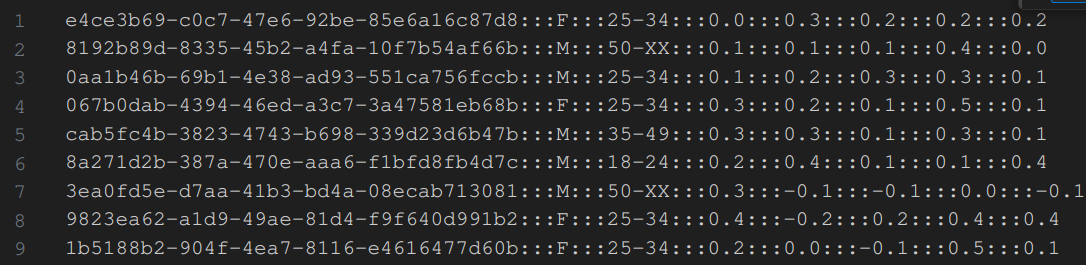
\includegraphics[width=\textwidth]{imaxes/formato_dataset.png}
  \caption{Formato archivo truth.txt \textit{dataset} 2015}
  \label{fig:formato-dataset}
\end{figure}

  \subsection{PAN author profiling 2016}
 Por otra parte, el conjunto de 2016 incluía una partición de entrenamiento formada por textos sacados de usuarios de Twitter y una partición de test formada por texto sacados de Blogs. Estos últimos utilizan un lenguaje más formal, habitualmente conteniendo poemas, canciones o fragmentos de texto no escritos por los usuarios etiquetados que podían afectar negativamente al rendimiento del algoritmo de perfilado. Por estas razones, se decidió utilizar únicamente la partición de entrenamiento para entrenar nuestro clasificador.
 
 El formato de este corpus es bastante similar al del 2015: cada autor aparece representado en un archivo .xml nombrado con un identificador único a partir del cual se puede sacar sus datos demográficos en un archivo truht.txt.
 
 La diferencia con el de 2015, está en que en vez de aparecer los tweets directamente en el .xml, aparecen las URLs a esos tweets. Además en vez haber exactamente 100 \textit{tweets} por autor, en la mayoría hay hasta 1000. Para conseguir los textos correspondientes a los \textit{tweets} el PAN disponía de un programa\footnote{\url{https://github.com/pan-webis-de/pan-code/tree/master/clef16/author-profiling/twitter-downloader}} que los descargaba y escribía directamente el texto de los mismos en los .xml. Sin embargo, desde 2020 la API de Twitter cambió y este programa dejó de funcionar\footnote{Enlace al issue de github donde lo indican: \url{https://github.com/pan-webis-de/pan-code/issues/3}}.
 
 Por este motivo, se decidió crear un web scraper que fuera leyendo las direcciones URL de los .xml que se correspondían con los tweets de los usuarios y descargara el texto de estos sin necesidad de usar la API de Twitter. Sin embargo, este proceso era mucho más lento que el uso del programa antes mencionado (1000 \textit{Tweets}/minuto frente a aproximadamente 30 \textit{Tweets}/minuto). Esto hizo que decidiera ejecutar de forma \textit{serveless} este programa diariamente en forma de notebook en Kaggle\footnote{\url{https://www.kaggle.com/}}, esta web permite programar ejecuciones de jupyter notebooks de forma asíncrona que pueden durar hasta 12 horas siendo 10 el número máximo de notebooks ejecutándose concurrentemente. De esta forma en un par de días ya tenía descargada toda la colección, sin contar los tweets y usuarios eliminados que eran bastantes. En la figura \ref{fig:scraper} se puede ver una captura de los logs resultantes de realizar una ejecución de 12 horas del \textit{scraper} para descargar los \textit{tweets} del \textit{dataset}.
 %En total hay 187995 tweets y 843.0269058295964 tweets por autor de media

 \noindent\begin{figure}[hp!]
  \centering
    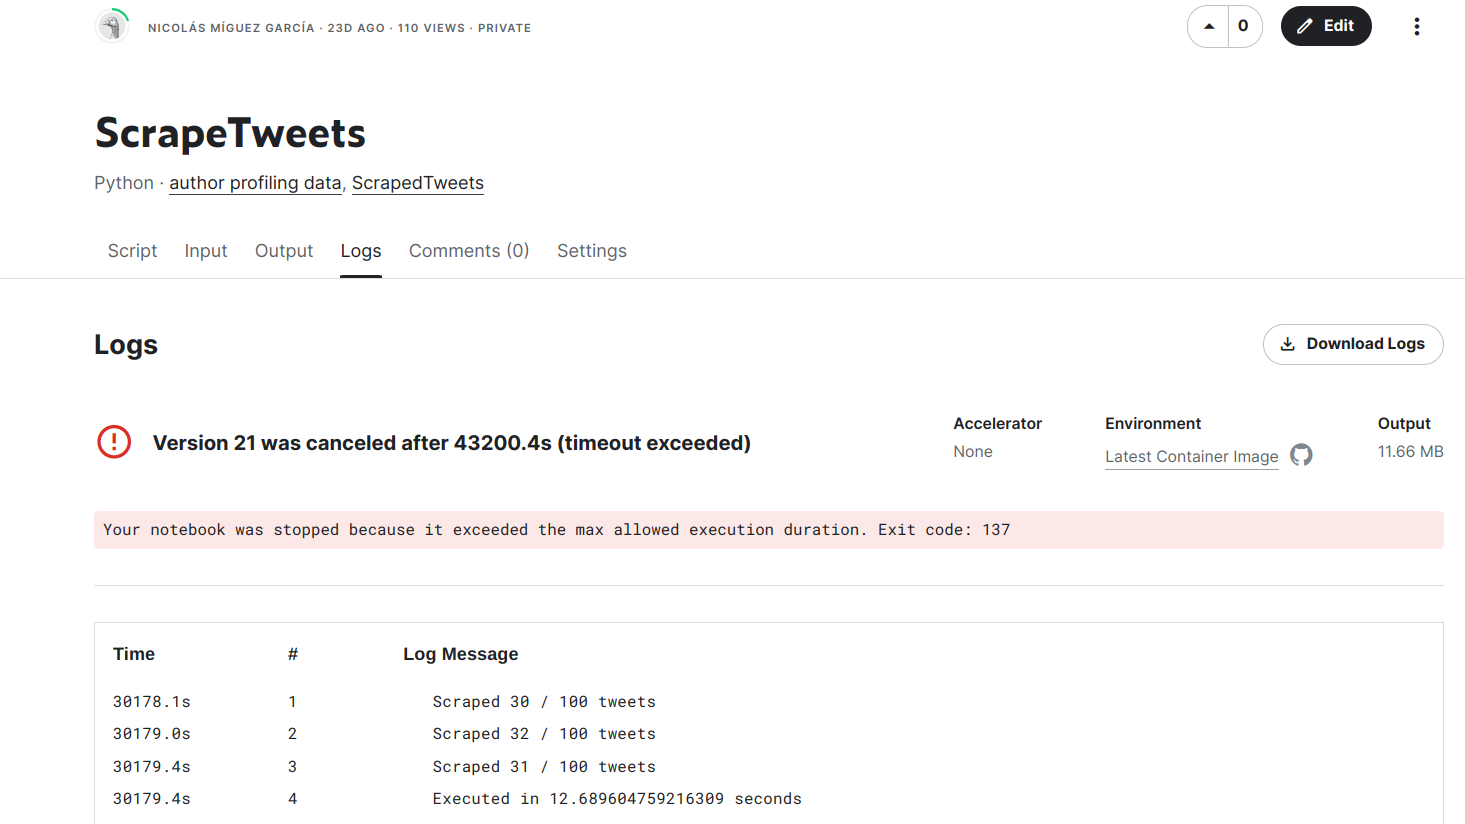
\includegraphics[width=\textwidth]{imaxes/scraper.png}
  \caption{Logs resultado de una ejecución del notebook a modo de \textit{scraper} para la obtención de los \textit{tweets} del \textit{dataset} de 2016}
  \label{fig:scraper}
\end{figure}
 
   \subsection{Distribución de usuarios de los \textit{dataset}}

   En la tabla \ref{tab:datasets_edad} podemos ver la distribución de autores en función de edad y género de ambos conjuntos. Como se puede observar los \textit{datasets} están equilibrados en cuestión de género, mientras que están bastante más desequilibrados en cuestión de edad.
   
   Vale la pena mencionar que aunque en el \textit{dataset} de 2016, originalmente había 250 de Training, al descargar los textos correspondientes a estos muchos de ellos no estaban disponibles (puesto que los \textit{tweets} eran se había publicado originalmente en el año 2013), pues se habían eliminado su cuenta de Twitter. Consecuentemente, descartando estos usuarios quedan un total de 222.
   \begin{table}[hp!]
    \centering
    \rowcolors{2}{white}{udcgray!25}
    \begin{tabular}{|l|ll|l|}
        \rowcolor{udcpink!25}
        \hhline{~|---}
        \multicolumn{1}{c|}{\cellcolor{white}} & \multicolumn{2}{c|}{\textbf{PAN-AP 2015}} & \textbf{PAN-AP 2016}\\ \hline
        Categoría & Training & Test & Training \\ \hline
        18-24 & 22 & 18 & 11\\
        25-34 & 46 & 44 & 54\\
        35-49 & 22 & 18 & 116\\
        +50 & 10 & 8 & 41\\ \hline
        Hombres & 50 & 44 & 111\\
        Mujeres & 50 & 44 & 111\\ \hline
        Total & 100 & 88 & 222\\ \hline  
    \end{tabular}%
    \caption{Distribución de usuarios en función de edad y género en los conjuntos de entrenamiento utilizados.}
    \label{tab:datasets_edad}
\end{table}

\section{Búsqueda y comparación de algoritmos}
En esta sección, se detalla la fase del proyecto consistente en 
 la investigación sobre los algoritmos o modelos existentes de clasificación de texto para tareas de perfilado automático de usuarios.
 
 El objetivo principal de esta fase era el análisis del estado del arte en este campo con la finalidad de escoger y replicar los algoritmos, de perfilado de usuario, más robustos para nuestro trabajo. En consecuencia, vale la pena resaltar que la intención no era realizar un modelo original desde cero sino utilizar uno ya implementado y del que se tenga conocimiento que reporta buenos resultados.
 
 Para ello, se orientó la búsqueda hacia las competiciones ya mencionadas en el apartado \ref{sec:estado_arte} como PAN (\cite{pan:2013}) o IberLef (\cite{iberlef2022}). Esto tiene dos motivos: primero que seleccionando los algoritmos de entre los participantes en una de estas competiciones, contamos con la información previa de la bondad de los algoritmos con los otros competidores, pudiendo así seleccionar los que mejor se comportaron en las mismas; por otra parte, estas competiciones al estar de alguna forma abiertas al público es más sencillo encontrar de forma pública las implementaciones de los algoritmos participantes en repositorios como Github\footnote{\url{https://github.com/}}.
 
En la tabla \ref{tab:comparacion-profilers} prueba se muestra una pequeña comparativa de los algoritmos del estado del arte con implementación disponible en Github. En ella se muestran en cada columna: la referencia a las \textit{working notes} del equipo participante de la tarea, la competición para la que se desarrolló, la posición final en la que quedó el equipo participante (teniendo en cuenta perfilado en idioma español solamente), el modelo de aprendizaje automático utilizado y un resumen muy general de las características extraídas para la clasificación del texto.

Como se puede ver en la tabla muchos de estos algoritmos usan modelos y características bastante similares entre ellos. En consecuencia, solo se decidieron replicar tres de ellos (\cite{loscalis22}, \cite{modaresi:2016} y \cite{grivas2015author}).


\begin{table}[hp!]
    \centering
    \rowcolors{2}{white}{udcgray!25}
    {
    \setlength{\tabcolsep}{0.4\tabcolsep}
        \begin{tabular}{|p{0.15\linewidth} |p{0.18\linewidth} |p{0.11\linewidth} |p{0.1\linewidth} | p{0.27\linewidth} |}
            \hline
            \rowcolor{udcpink!25}
            
            \textbf{Equipo} & \textbf{Competición}  & \textbf{Posición} & \textbf{Modelo} & \textbf{Características}\\ \hline
            Grivas \cite{grivas2015author} & PAN 2015 \cite{pan:2015} & 3º & \gls{svm} & Tfidf n-grams stylistic features\\
            Modaresi \cite{modaresi:2016} & PAN 2016 \cite{pan:2016} & 2º & \gls{lr} & Tfidf n-grams stylistic features\\
            Daneshvar \cite{Daneshvar2018} & PAN 2018 \cite{pan:2018} & 1º & \gls{svm} & Tfidf ngrams w LSA\\
            Bacciu \cite{bacciu2019bot} & PAN 2019 \cite{pan:2019} & 3º & \gls{svm} & Tfidf n-grams w LSA\\
            Baseline & PAN 2020 \cite{pan:2020} & & \gls{lr} & Tfidf n-grams\\
            LosCalis \cite{loscalis22} & IberLef 2022 \cite{iberlef2022} & 1º & \gls{mlp} & Embeddings (BERT + RoBERTa)\\
            Holgado \cite{holgado2022halbert} & IberLef 2022 \cite{iberlef2022} & 5º & \gls{em} & n-grams + embeddings + stylistic features\\ \hline
        \end{tabular}
    }
    \caption{Comparación de algoritmos del estado del arte en perfilado de usuarios de los cuales se encontró la implementación disponible en Github.}
    \label{tab:comparacion-profilers}
\end{table}

\subsection{Primera aproximación}
En primer lugar, tenemos al ganador de la competición del IberLef 2022: "PoliticEs 2022: Perfilado de usuarios para ideología política". Esta competición consistía en la predicción de género, profesión e ideología política binaria (izquierda y derecha) y multiclase (izquierda, centro-izquierda, centro-derecha y derecha) de usuarios de Twitter sobre un corpus de \textit{tweets} procedentes de periodistas, políticos y españoles.

En esta competición \cite{iberlef2022}, la mayoría de aproximaciones usadas por los participantes eran modelos basados en transformers \cite{vaswani2017attention}. Estos consistían en modelos de lenguaje pre-entrenados (BETO \cite{BETO}, MarIA \cite{MarIA}, BERT multilingüe, ALBERT...) afinados con el corpus de la competición, con el objetivo de extraer características del texto a nivel de documento. Este tipo de arquitecturas, basadas en transformers, son la gran novedad con respecto a los enfoques utilizados en competiciones de años anteriores del PAN. \\

%%%%%%%%%%%%%%%%%%%%%%%%%%%%%%%%%%%%%%%%%%%%%%%%%%%%%%%%%%%
% \subsubsection{Transformers y modelos de lenguaje}
% TODO 
% meter teoría sobre transformers y modelos de lenguaje
%%%%%%%%%%%%%%%%%%%%%%%%%%%%%%%%%%%%%%%%%%%%%%%%%%%%%%%%%%%

El enfoque utilizado por LosCalis \cite{loscalis22} por tanto, combinaba el modelo BERT \cite{devlin2019bert} pre-entrenado en idioma español, conocido como BETO \cite{BETO} junto con el modelo RoBERTa pre-entrenado en español, llamado MarIA \cite{MarIA}. Este emplea ambas arquitecturas para extracción de características a nivel de documento y en base a estas se entrena un perceptrón multicapa para decodificar las etiquetas de los usuarios. En la figura \ref{fig:arquitectura} se muestra la arquitectura del modelo utilizado.

\noindent\begin{figure}[hp!]
  \centering
    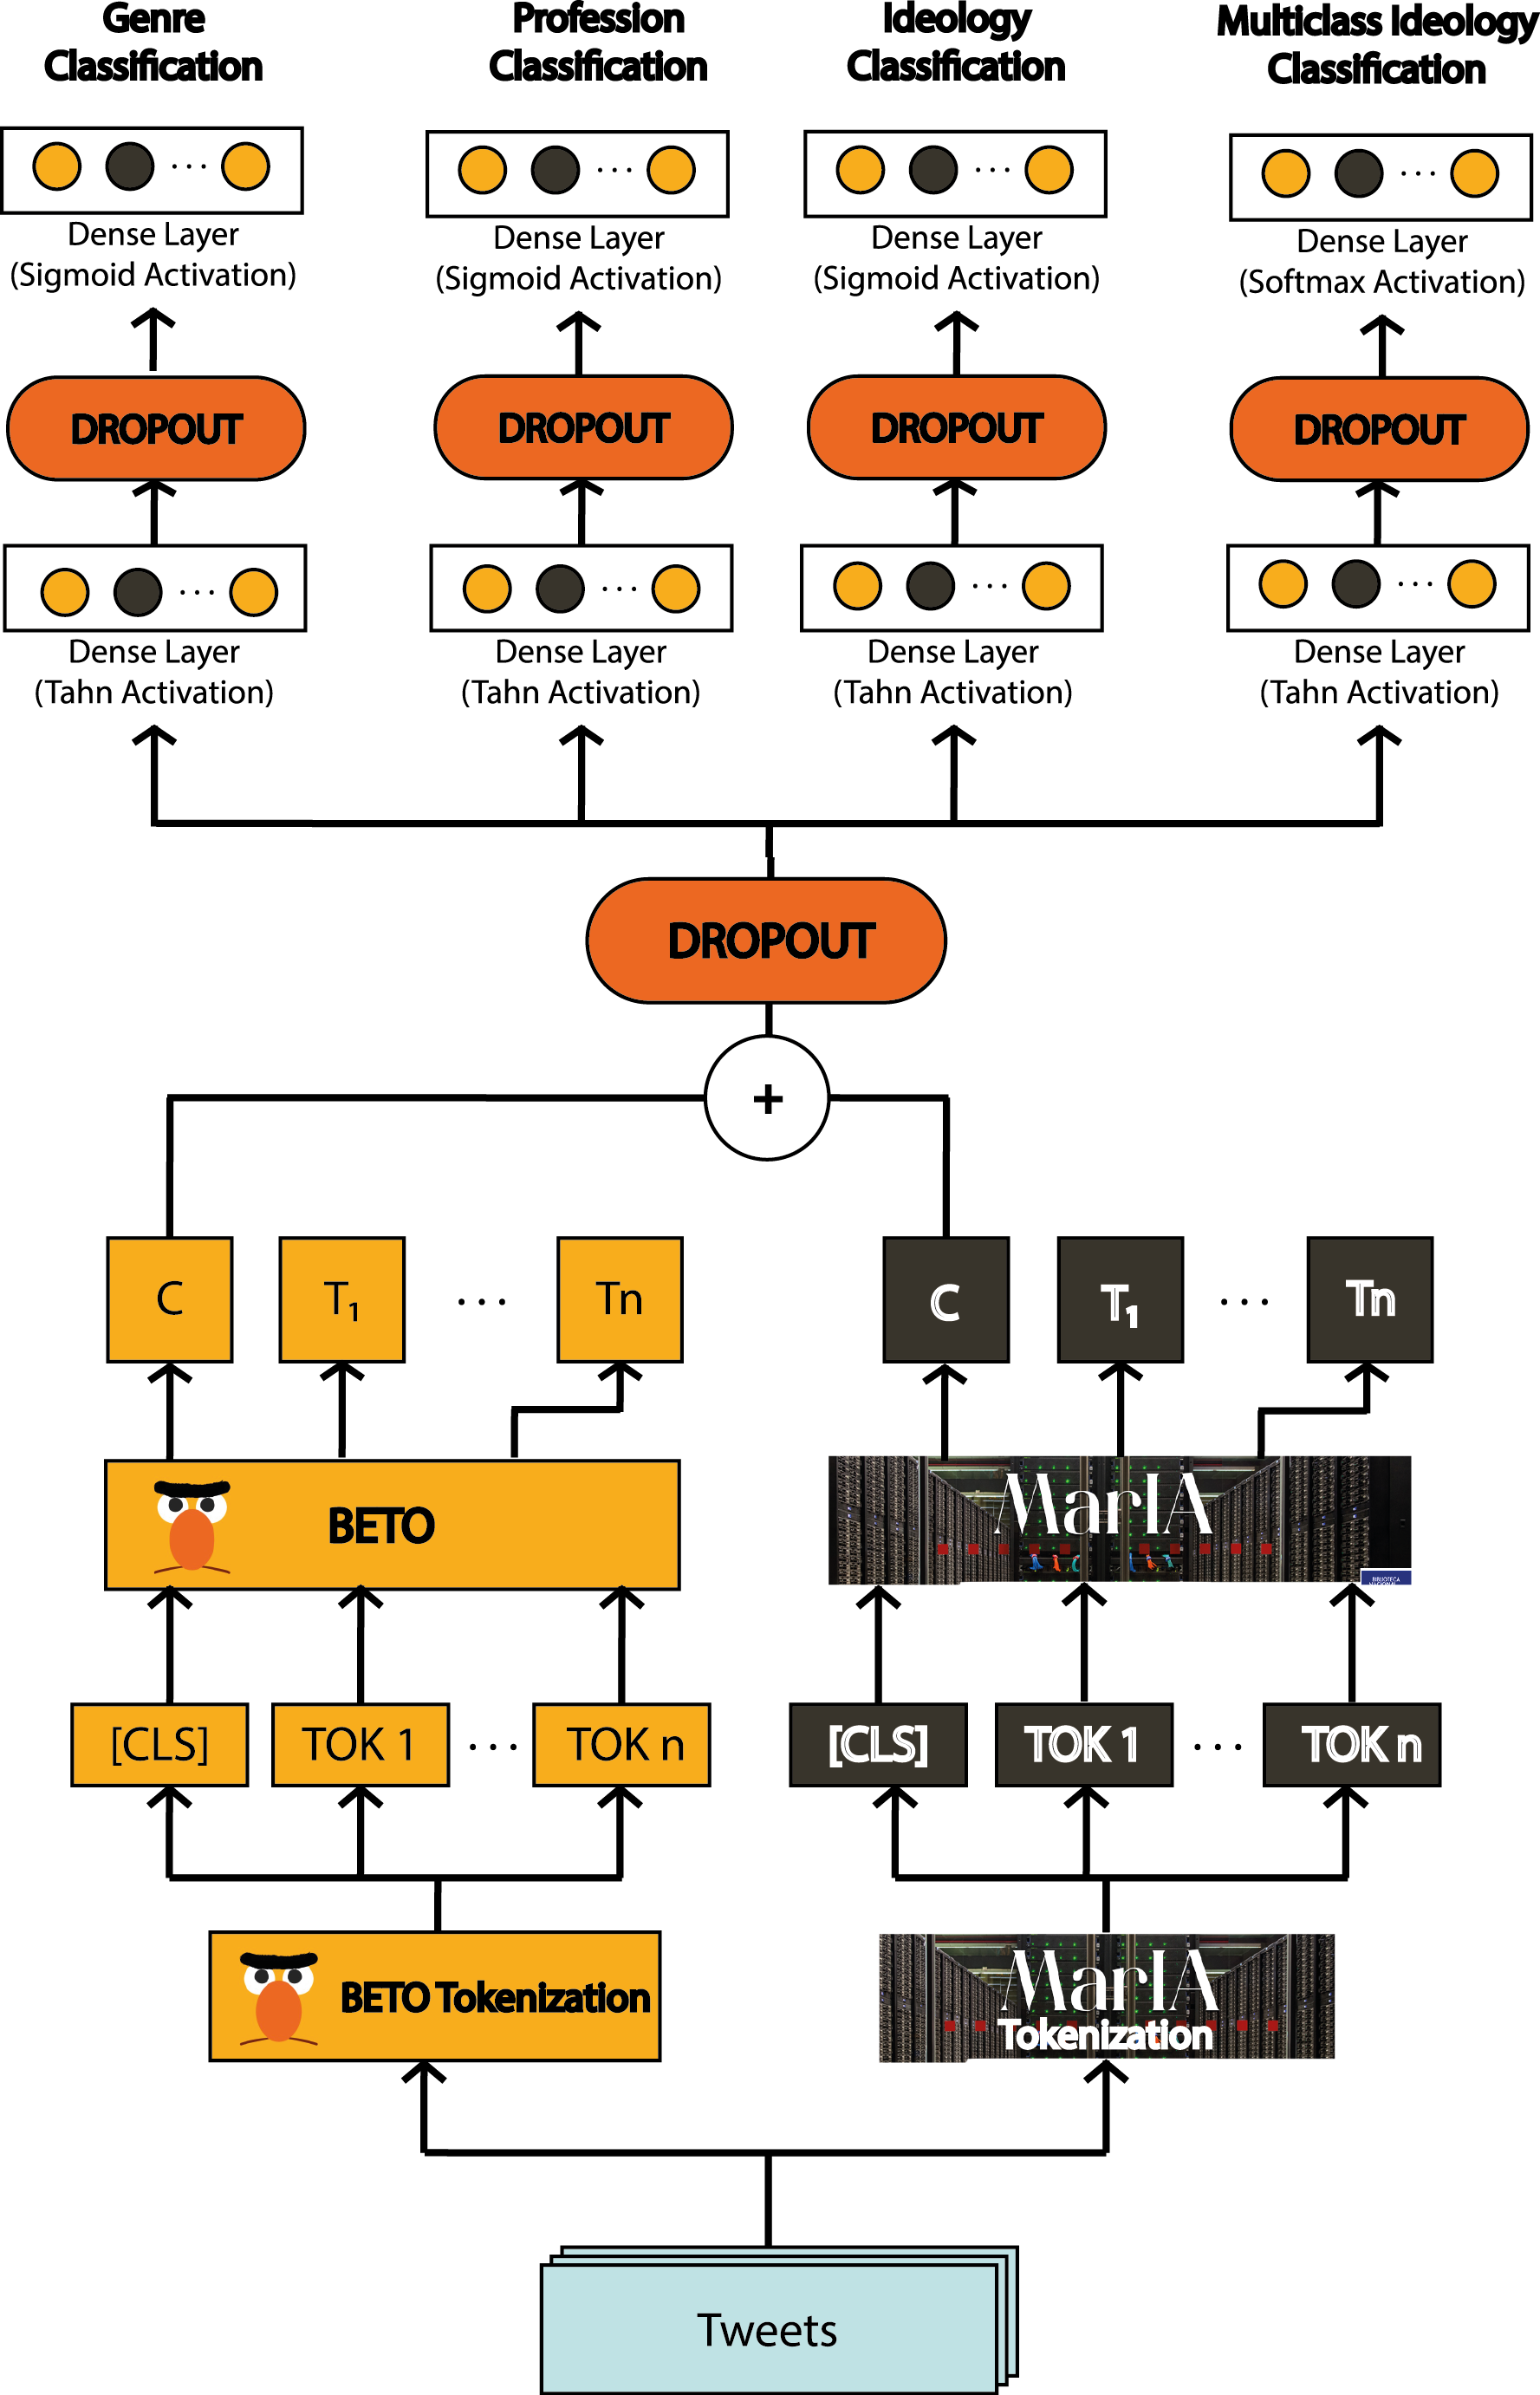
\includegraphics[height=0.8\textwidth]{imaxes/arquitectura_.png}
  \caption{Arquitectura del modelo ganador de la competición de Political Author Profiling del IberLef 2022, utilizado por LosCalis \cite{loscalis22}.}
  \label{fig:arquitectura}
\end{figure}

\subsubsection{Preprocesado}

Por una parte está el preprocesado realizado a la hora de la creación del corpus por los organizadores de la competición. Este consistió en descartar \textit{retweets}, \textit{tweets} donde se parafrasean titulares de periódicos o \textit{tweets} en otros idiomas distintos del español. Además de esto, se anonimizó la colección sustituyendo las menciones a usuarios por el token "@user".\\
Por otro lado, el preprocesado efectuado por LosCalis se limitó a la agrupación de los \textit{tweets} de un mismo autor en bloques de máximo 512 tokens tras la tokenización con BERT y RoBERTa. Esto es así debido a que los modelos basados en BERT no aceptan entradas de mayor tamaño.\\
En nuestro caso, se realizó un preprocesado parecido con la excepción de que se mantuvieron todos los \textit{tweets} de la colección aunque contuvieran fragmentos en otros idiomas o parafrasearan titulares de noticias o blogs. Por un lado, esto se hizo debido a que nuestros \textit{datasets} cuentan con un volumen mucho menor de textos en relación a los corpus de la competición del IberLef, por esa razón decidimos no realizar esa limpieza para mantener un corpus lo más grande posible.

Por otro lado, también se optó por sustituir las \textit{urls} encontradas por el token '<URL>', debido a que en el corpus de la competición no se incluían estas tampoco. Además, se optó por sustituir los emoticonos encontrados en el texto por el token '<EMOTICON>' y los emojis por su descripción sacada de la librería emoji\footnote{\url{https://pypi.org/project/emoji/}}.

\subsubsection{Modelo}
En nuestro caso se replicó el mismo modelo usado por los participantes de la tarea, con las adaptaciones debidas para en las salidas de la red neuronal. En el caso de LosCalis, tenían tres salidas binarias (género, profesión, ideología binaria) y una multiclase (ideología multiclase). En nuestro problema, se tienen únicamente dos salidas: género y edad. En consecuencia se utilizó la arquitectura que se puede ver en la figura \ref{fig:arquitectura_adaptada}. En ella se muestra que se mantienen las mismas capas y funciones de activación que en la arquitectura original con la diferencia de que en vez de cuatro bloques separados de decodificación de las etiquetas, ahora tenemos únicamente dos.

\noindent\begin{figure}[hp!]
  \centering
    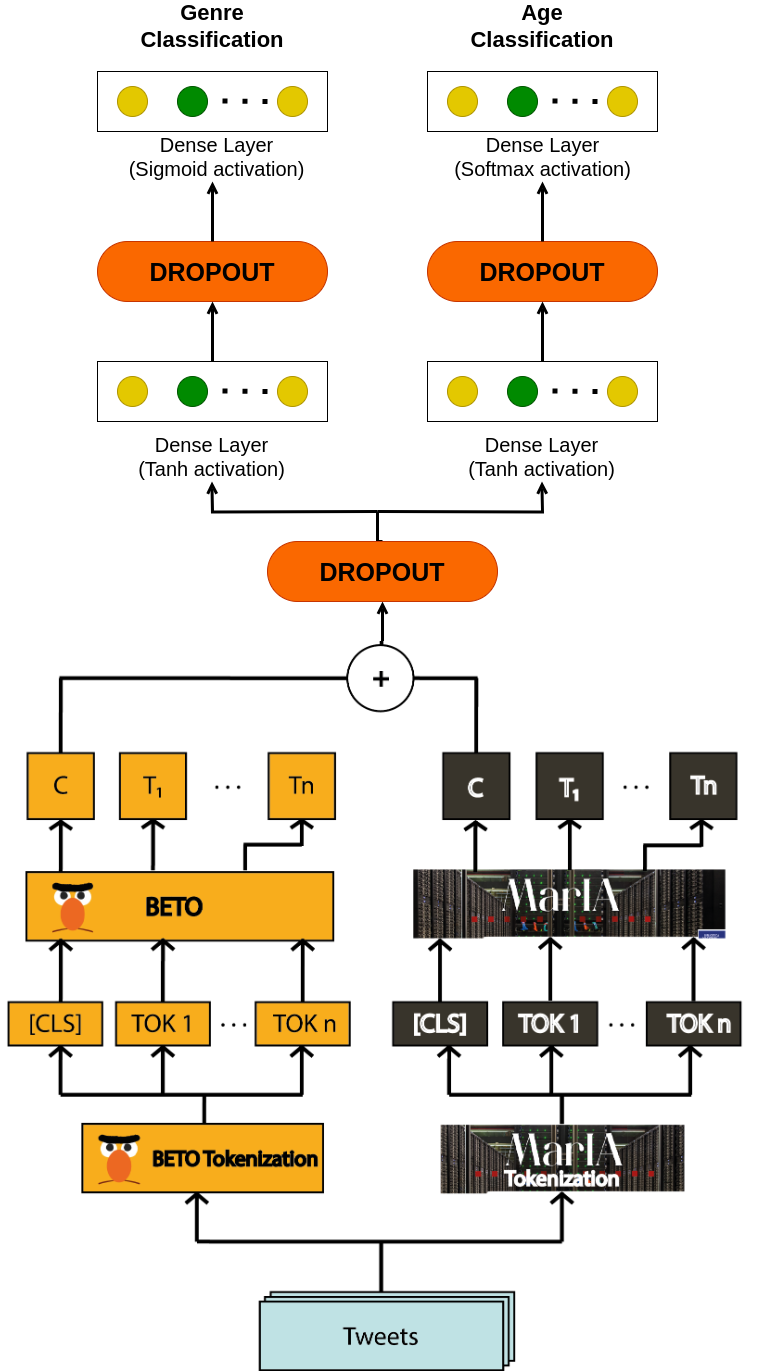
\includegraphics[height=0.8\textwidth]{imaxes/diagrama_arquitectura_profiler.png}
  \caption{Arquitectura basada en transformers adaptada de la aproximación de \cite{loscalis22}.}
  \label{fig:arquitectura_adaptada}
\end{figure}

\subsubsection{Experimentos realizados}
Se realizaron distintas pruebas con los conjuntos de datos expuestos en la sección \ref{sec:datasets}. Para estas se utilizaron la misma configuración de hiper-parámetros propuesta por \cite{loscalis22}, que se puede ver en la tabla \ref{tab:hiperparametros}. 

\begin{table}[hp!]
    \centering
    % \rowcolors{2}{white}{udcgray!25}
    \begin{tabular}{ll}
        \hline
        % \rowcolor{udcpink!25}
        \textbf{Parámetro}  & \textbf{Valor} \\ \hline
        Train batch size    & 64             \\
        Predict batch size  & 8              \\
        Learning rate       & 3e-5           \\
        Training epochs     & 5              \\
        Max sequence lenght & 512            \\
        Dropout             & 0.15           \\
        Optimizer           & Adam           \\
        Dense layer units   & 768            \\ \hline
    \end{tabular}
    \caption{Hiperparámetros utilizados en los experimentos realizados, propuestos por \cite{loscalis22}}
    \label{tab:hiperparametros}
\end{table}
En la tabla \ref{tab:resultados-bert} se pueden ver los experimentos realizados así como los resultados obtenidos en cada uno de ellos en términos de precisión para género y edad.

\begin{table}[hp!]
    \centering
    \rowcolors{2}{white}{udcgray!25}
    \resizebox{\textwidth}{!}{
        \begin{tabular}{|l|l|l|l|}
            \rowcolor{udcpink!25}
            \hline
            \textbf{Entrenamiento} & \textbf{Test} & \textbf{Género} & \textbf{Edad}\\ \hline
            Training 2015     & Test 2015         & 0.8863   & 0.6250\\
            2015 (Train+Test) & Training 2016     & 0.4865   & 0.2703\\
            Training 2016     & 2015 (Train+Test) & 0.4468   & 0.3191\\
            Training 2016     & Test 2016         & 0.4545   & 0.4181\\ \hline
        \end{tabular}
    }
    \caption{Precisión para género y edad en distintos experimentos realizados utilizando el enfoque propuesto por \cite{loscalis22} con las particiones de entrenamiento y test de las competiciones de PAN de 2015 y 2016.}
    \label{tab:resultados-bert}
\end{table}

Lo primero que llama la atención de estos resultados es la diferencia de rendimiento obtenida usando el \textit{dataset} de 2015, a modo de réplica de la competición del PAN \cite{pan:2015}, con el resto de experimentos realizados.

En el primer caso los resultados obtenidos no se alejan demasiado de los conseguidos por el equipo ganador de la misma: 0.9659 y 0.7955, para género y edad respectivamente.

Sin embargo, cuando se trata de aumentar estos datos para obtener mejores resultados, por ejemplo usando el \textit{dataset} completo de 2015 (entrenamiento y test) para entrenar el modelo y se prueban a predecir los autores del corpus de entrenamiento del 2016 se puede ver como los resultados obtenidos empeoran considerablemente, hasta el punto de ser peores que un clasificador aleatorio. Esto se repite al entrenar con la partición de Training de 2016 y testear con la de 2015 completa o con la de Test de 2016 (competición PAN 2016).

Para solventar este problema, lo primero que se probó fue separar una parte del conjunto de entrenamiento para usarlo como conjunto de validación, con la finalidad de observar como se comportaba la función de pérdida o loss\footnote{}, de la red.
\\ La función de pérdida en aprendizaje automático mide la discrepancia entre la clasificación de las predicciones de la red y los datos reales. En las redes neuronales, el objetivo del entrenamiento consiste en la minimización del valor de esta función en cada ciclo mediante del ajuste del valor de los pesos de las conexiones de la red, por medio del algoritmo de retro-propagación del error. Como se explica en \cite{janocha2017loss}, existen diversas alternativas a la hora de escoger una función de pérdida, sin embargo, para problemas de clasificación es bastante común el uso de la entropía cruzada (pérdida logarítmica), por lo cual es la elegida para nuestro algoritmo.

De esta forma viendo la evolución de la función de pérdida durante el entrenamiento, se podría saber si el sistema estaba sobre-entrenado o no. Pues bien, los resultados de esta prueba se pueden ver en la figura \ref{fig:loss}.
\\
 \begin{figure}[hbtp!]
    \centering
    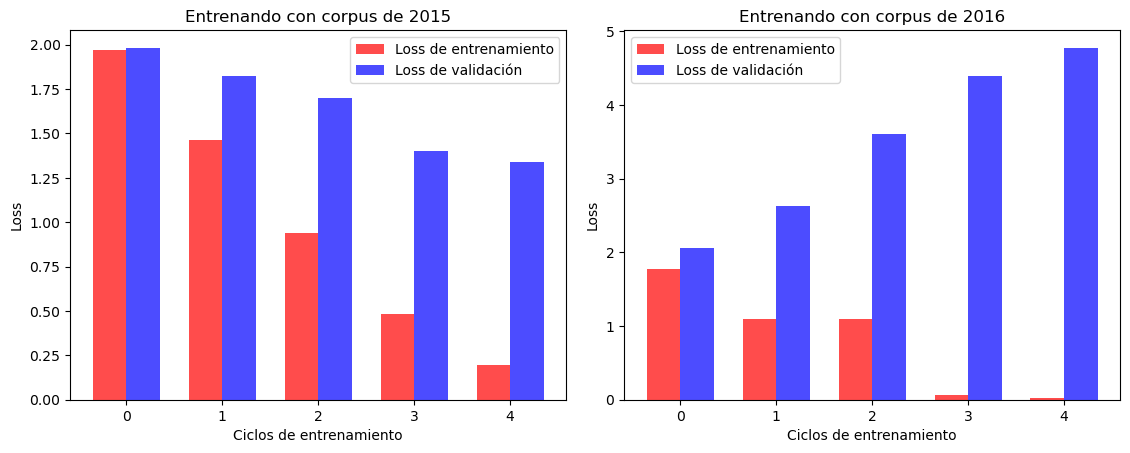
\includegraphics[width=\textwidth]{imaxes/loss.png}
    \caption{Evolución del loss de entrenamiento y validación del modelo propuesto por LosCalis al entrenar con los \textit{datasets} de 2015 y 2016.}
    \label{fig:loss}
\end{figure}
Como se puede ver a la hora de entrenar el modelo con los datos de 2015 el loss del conjunto de validación disminuía al mismo tiempo que el loss del conjunto de entrenamiento; sin embargo, a la hora de entrenar usando el corpus de entrenamiento de 2016 pasaba justo lo contrario, el loss de validación aumentaba cada ciclo mientras el de entrenamiento disminuía (signo de que el modelo se está sobre-ajustando a los datos de entrenamiento y no consigue generalizar).

 Tras descubrir esto, lo primero que se me ocurrió fue investigar un poco los dos conjuntos y compararlos para descubrir si existía alguna diferencia entre ellos. Lo que se descubrió fue que probablemente en el \textit{dataset} de 2015, tanto en el conjunto de entrenamiento como en el de test existían autores repetidos, de modo que el modelo obtenía buenos resultados debido a que el modelo se aprendía el las características textuales de usuarios concretos y no a distinguir la edad o género de una persona aleatoria.
 
 Por otro lado, la diferencia de rendimiento entre el modelo adaptado a nuestro problema y el propuesto por \cite{loscalis22} se especula que se deba probablemente a el mayor tamaño del corpus usado para entrenar en la competición del IberLef (alrededor de 400.000 \textit{tweets} de más de 700 usuarios distintos, frente a 222 usuarios con aproximadamente 800 tweets cada uno) unido a un vocabulario más formal usado por políticos y periodistas españoles junto a unas temáticas mucho más menos variadas, comparado con el vocabulario del usuario promedio de twitter lleno de expresiones de jerga, abreviaturas y disparidad de temáticas tratadas.
 
 Debido a estos malos resultados obtenidos y a la falta de un corpus de mayor tamaño necesario para entrenar un modelo complejo basado en aprendizaje profundo, se decidió orientar el trabajo hacia modelos más sencillos como los expuestos a continuación.



\subsection{Segunda aproximación}
Por otro lado el segundo algoritmo de perfilado probado es el correspondiente a \cite{grivas2015author}. Este obtuvo la tercera posición, en general, en la tarea de author profiling de PAN 2015 (\cite{pan:2015}).
Los \textit{\textbf{datasets}} usados en la competición son los explicados en la subsección \ref{subsec:pan15}.
\subsubsection{Preprocesado}
El preprocesado realizado es distinto dependiendo del tipo de características extraídas. Así los autores de este trabajo separan por un lado características estructurales y características estilométricas.

Las primeras incluyen el numero de menciones, \textit{hashtags} y URLs que contienen los \textit{tweets}. Las segundas, se refieren a la longitud del \textit{tweet} en caracteres y tf-idf n-grams.

Para las estructurales no se realizó ningún preprocesado del texto a parte de concatenar todos los tweets de un autor. Por otro lado, para las estilométricas se eliminaron cualquier tag HTML encontrado, URLs, menciones así como los caracteres '\#' de los \textit{hashtags}.

\subsubsection{Modelo}
Para la clasificación del género, se usó una \gls{svm} con kernel rfb, y se usaron como características únicamente los tf-idf n-grams. En cuanto a la edad, se usó una \gls{svm} con kernel linear a la que se le pasaron como características: tf-idf ngrams, longitud del \textit{tweet}, número de URLs, menciones y \textit{hashtags}. Además, se compensó el desbalanceo de los distintos grupos de edad mediante pesos inversamente proporcionales a la frecuencia de las clases.

\subsubsection{Experimentos y resultados}
En la tabla \ref{tab:aprox2_results} se pueden observar los resultados de los experimentos realizados en esta aproximación. Las métrica elegida tanto para género como edad es la precisión, debido a que es la que se usaba en la competiciones del PAN 2015 y 2016.

\begin{table}[hp!]
    \centering
    \rowcolors{2}{white}{udcgray!25}
    {%
    \setlength{\tabcolsep}{0.6\tabcolsep}
    \begin{tabular}{|l|ll|ll|}
        \hline
        \rowcolor{udcpink!25}
        \textbf{N-gram} & \textbf{Entrenamiento} & \textbf{Test} & \textbf{Género} & \textbf{Edad} \\ \hline
        Carácter [3, 3] & Training 2015 & Test 2015 & 0.9091 & \textbf{0.7159} \\
        Carácter [3, 5 ] & Training 2015 & Test 2015 & \textbf{0.9205} & 0.6932 \\ \hline
        Carácter [3, 3] & Training 2015 & Training 2016 & 0.5766 & 0.3423 \\
        Carácter [3, 3] & Training 2015 & Training 2016 & 0.5856 & 0.3018 \\
        Carácter [3, 3] & 2015 (Train+Test) & Training 2016 & 0.5405 & 0.3468 \\
        Carácter [3, 5] & 2015 (Train+Test) & Training 2016 & 0.5586 & 0.2972 \\ \hline
        Carácter [3, 5] & Training 2016 & 2015 (Train+Test) & 0.5638 & 0.4627 \\ \hline
        Carácter [3, 5] & Training 2016 & Test 2016 & 0.5091 & 0.4545 \\ \hline
        Carácter [3, 3] & Training 2016 & *10-Fold CV & 0.6712 & \textbf{0.5045} \\
        Carácter [3, 5] & Training 2016 & *10-Fold CV & 0.6757 & \textbf{0.5045} \\
        Carácter [5, 8] & Training 2016 & *10-Fold CV & 0.6667 & \textbf{0.5045} \\
        Palabra  [1, 3] & Training 2016 & *10-Fold CV & \textbf{0.6937} & 0.4910 \\ \hline
        Carácter [3, 3] & 2015+2016 (Train) & *10-Fold CV & 0.7024 & 0.6073 \\
        Carácter [3, 5] & 2015+2016 (Train) & *10-Fold CV & \textbf{0.7170} & 0.5707 \\
        Carácter [5, 8] & 2015+2016 (Train) & *10-Fold CV & \textbf{0.7170} & \textbf{0.6195} \\
        Palabra  [1, 3] & 2015+2016 (Train) & *10-Fold CV & 0.6610 & 0.5390 \\
        Palabra  [1, 1] & 2015+2016 (Train) & *10-Fold CV & 0.7122 & 0.5829\\ \hline
        \end{tabular}%
    }
    \caption{Resultados en términos de precisión para género y edad de los experimentos realizados para la aproximación 2 (modelo propuesto por grivas).}
    \label{tab:aprox2_results}
\end{table}
Una vez más sucede que los resultados obtenidos de replicar la competición del PAN 2015, son mucho mejores que el resto de experimentos realizados, lo que afianza la teoría de que en ese \textit{dataset} existen autores repetidos.

Por otro lado, esta aproximación reporta mejores resultados tanto en género como en edad en el resto de experimentos realizados. Por ejemplo al entrenar con el dataset de 2016 y hacer test con 2015 el perfilador ya es ligeramente mejor que un clasificador aleatorio: 56\% y 46\% de precisión para género y edad respectivamente. Lo que refuerza la idea de que en caso de disponer de un corpus de tamaño relativamente pequeño los modelos tradicionales más sencillos son preferibles a los grandes modelos de lenguaje basadose en aprendizaje profundo y transformers que están de moda actualmente.

Los resultados de replicar la competición de PAN 2016 (entrenamiento 2016 y test 2016) muestran como este modelo no generaliza bien a otros géneros a parte de Twitter como son los textos de Blogs, utilizados en el \textit{dataset} de Test de 2016.

Para finalizar, en las últimas filas de la tabla se investigó acerca del tipo de características basadas en n-grams que mejor funcionaban en estos \textit{datasets}. Para ello se utilizó un 10-fold Cross-Validation con el dataset de training de 2016 y el dataset de training de 2016 sumado al de 2015 completo (Training y Test). El cross-validation se utilizó en parte para evitar el sesgo de que pueda haber autores repetidos en los datos del 2015 y porque en 2016 la partición de Test contenía textos de un género distinto (textos de Blogs) que la de entrenamiento. Los resultados que se sacan de estos experimentos son que los n-grams basados en secuencias de 1-3 palabras son las que mayor precisión alcanzan para la predicción de género. Mientras que, los n-grams basados en secuencias de  5-8 caracteres son las que mejores resultados obtienen para edad. No obstante, entre los rangos probados no hay una diferencia significativa de rendimiento en la clasificación.
\subsection{Tercera aproximación}
El último perfilador analizado es el correspondiente al trabajo de \cite{modaresi:2016}. Este fue propuesto para la competición del PAN 2016. En ella los participantes debían realizar un modelo que predijese el género y edad de autores de textos sacados de Blogs\footnote{\url{https://www.blogger.com/about/}} habiendo entrenado el mismo mediante textos sacados de usuarios de Twitter (\ref{sec:datasets}). Por lo tanto, ese algoritmo debe ser lo más independiente del género de escritura posible, lo cual es beneficioso para nuestro problema, ya que entrenamos con textos sacados de una red social como Twitter para predecir usuarios de Reddit.

En esta competición los resultados fueron bastante bajos comparados con las anteriores: el autor de este modelo (\cite{modaresi:2016}), el cual quedó en segunda posición en idioma español, obtuvo 0.6964 y 0.5179 para género y edad respectivamente.

\subsubsection{Preprocesado}
El procesado realizado en este algoritmo, tenía la intención de eliminar la información específica de género presente en los textos. De se usaron distintas operaciones de preprocesado en función de las características extraídas del texto. A continuación se enumeran todas las operaciones de preprocesado que se realizan para el perfilado:
\begin{itemize}
    \item p1: Pasar el texto a minúsculas.
    \item p2: Filtrar cualquier URL encontrada.
    \item p3: Eliminar menciones en las que aparezca un nombre de usuario del tipo '@username'.
    \item p4: Eliminar todos los Hashtags del texto.
    \item p5: Eliminar los retweets encontrados (en teoría no existen en el \textit{dataset}).
    \item p6: Eliminar cualquier carácter no latino encontrado.
    \item p7: Eliminar acentos latinos de palabras, para favorecer la precisión de características basadas en n-grams.
    \item p8: Eliminar caracteres no alfabéticos, como aquellos encontrados en emojis.
    \item p9: Eliminar stop-words basadas en una lista predefinida. 
\end{itemize}
Además de estas operaciones se procedió a la típica operación de concatenar los texto procedentes de un mismo autor para la extracción de características.

\subsubsection{Características extraídas}
En la tabla \ref{tab:preprocesado} se especifican las operaciones que se realizaron para cada tipo de característica extraída. A continuación se explica en que consisten estas:
\begin{table}[hp!]
    \centering
    \rowcolors{2}{white}{udcgray!25}
    \begin{tabular}{|l|l|}
        \rowcolor{udcpink!25}
        \hline
        \textbf{Característica} & \textbf{Operaciones de preprocesado} \\\hline
        Unigrams & p9 ◦ p8 ◦ p7 ◦ p6 ◦ p5 ◦ p4 ◦ p3 ◦ p2 ◦ p1 \\
        Bigrams & p8 ◦ p7 ◦ p6 ◦ p5 ◦ p4 ◦ p3 ◦ p2 ◦ p1 \\
        Promedio de errores de escritura & —— \\
        N-grams de caracteres & p2 ◦ p3 ◦ p4 ◦ p1 \\
        Características de puntuación & —— \\ \hline
    \end{tabular}%
    \caption{Operaciones de preprocesado realizadas según la característica extraída del texto.}
    \label{tab:preprocesado}
\end{table}
\begin{itemize}
    \item \textbf{Unigrams} y \textbf{Bigrams}: consisten en secuencias de n-grams basadas en palabras de longitud uno y dos respectivamente.
    \item \textbf{Promedio de errores de escritura}: se determina un valor relativo para las palabras correctamente escritas y se va sumando, de modo que cuanto mayor sea esta suma en relación a la longitud del texto, menores errores de escritura habrá.
    \item \textbf{N-grams de caracteres}: en concreto se utilizan secuencias de longitud 4, de caracteres con límites, es decir, los caracteres de la secuencia deben pertenecer todos a la misma palabra.
    \item \textbf{Puntuación}: además se mide el número promedio de comas, puntos y marcas de exclamación del texto.
\end{itemize}
Para la predicción de la edad se usaron todas estas características, para el género se omitió la puntuación.

\subsubsection{Modelo}
En este algoritmo, se probó con diferentes técnicas como Gradient Boosting o Random Forests, sin embargo los resultados obtenidos por medio de Regresión Logística fueron superiores. Por ello se empleó este modelo.\\
Se usa la estrategia uno frente a todos para la clasificación multiclase de la edad. Ademñas se establece el hiperparámetro $C=10^{-3}$.
\subsubsection{Experimentos y resultados}
En la tabla \ref{tab:results_aprox3} se muestran los experimentos realizados en esta aproximación. Como en las anteriores la métrica utilizada es la precisión.

\begin{table}[hp!]
    \centering
    \rowcolors{2}{white}{udcgray!25}
    {
    \setlength{\tabcolsep}{0.6\tabcolsep}

    \begin{tabular}{|l|l|ll|ll|}
        \hhline{------}
        \rowcolor{udcpink!25}
          \multicolumn{2}{|c|}{Dataset} & \multicolumn{2}{c|}{Género} & \multicolumn{2}{c|}{Edad} \\ \hline
        \textbf{Entrenamiento} & \textbf{Test} & \textbf{Acc} & \textbf{F1} & \textbf{Acc} & \textbf{F1}\\ \hline
        Training 2015 & Test 2015 & 0.8977 & 0.8977 & 0.5795 & 0.5795 \\
        2015 (Train+Test) & Training 2016 & 0.6368 & 0.6368 & 0.3722 & 0.3722\\
        Training 2016 & 2015 (Train+Test) & 0.6968 & 0.6968 & 0.3830 & 0.3830 \\
        Training 2016 & Test 2016 & 0.5818 & 0.5818 & 0.5090 & 0.5090 \\
        Training 2016 & *10-Fold CV & 0.7657 & 0.7657 & 0.5124 & 0.5124 \\
        2015+2016 (Train) & *10-Fold CV & 0.8173 & 0.8173 & 0.6423 & 0.6423\\ \hline
    \end{tabular}%
    }
    \caption{Resultados en términos de precisión para género y edad de los experimentos realizados para la aproximación 3 (modelo propuesto por modaresi).}
    \label{tab:results_aprox3}
\end{table}

En esta ocasión se puede ver como sigue el patrón de resultados muy buenos para el benchmark de la competición del PAN 2015: género alrededor de 90\% de precisión, y para la edad en este caso los resultados son bastante peores que en con los otros dos modelos.

Sin embargo, esta aproximación mejora a las otras dos en cuanto al perfilado para géneros distintos (entrenamiento y test 2016), donde vemos que el género ya supera el 50\% de precisión y la edad lo alcanza también.

En líneas generales, se puede observar que esta aproximación mejora significativamente a las otras dos en la predicción del género sobre todo, pues consigue una precisión media de 76\% para el 10-fold Cross-Validation del \textit{dataset} de 2016 y llega al 81\% si añadimos el corpus del 2015, frente al 69\% y 71\% de la aproximación 2. En cuanto a la predicción de la edad no obstante, no se aprecia una mejora significativa con respecto a la segunda aproximación.


% \begin{table}[hp!]
%     \centering
%     \rowcolors{2}{white}{udcgray!25}
%     \begin{tabular}{llll}
%         \rowcolor{udcpink!25}
%         \multicolumn{3}{c}{\textbf{PAN 2015}}              \\ \hline
%         Modelo         & Gender          & Age             \\ \hline
%         Aproximación 1 & 0.8863          & 0.6250          \\
%         Aproximación 2 & 0.9091          & 0.7159          \\
%         Aproximación 3 & 0.8977          & 0.5795          \\ \hline
%         Ganador        & \textbf{0.9659} & \textbf{0.7955} 
%     \end{tabular}
%     \caption{}
% \label{tab:my-table}
% \end{table}
 \chapter{Tecnologías utilizadas}
\label{chap:tecnologias}
\lettrine{E}{n} este capítulo se presentan las herramientas tecnológicas utilizadas durante el desarrollo de este trabajo, al igual que la justificación de su elección sobre otras alternativas.\\
En primer lugar, se presentan las herramientas tecnológicas empleadas para el desarrollo y entrenamiento de los modelos de perfilado automático seleccionados. Por otro lado, tenemos las herramientas utilizadas para la construcción de la aplicación web. Por último, se exponen las herramientas ayuda al desarrollo que se han utilizado transversalmente durante todo el proceso software.\\

\section{Algoritmos de perfilado}
En esta sección se muestran las herramientas empleadas para la creación y entrenamiento de los modelos de perfilado automático, así como para la extracción, carga y preprocesado de los conjuntos de datos de entrenamiento y test.
\subsection{Python}
\label{subsec:python}
Python\footnote{\url{https://www.python.org/}} es un lenguaje de programación de alto nivel, interpretado y multiparadigma. Actualmente es uno de los lenguajes de programación más populares en diversos ámbitos como la ciencia y análisis de datos, inteligencia artificial y programación web. Algunas de las razones por las que es tan popular son: su sintaxis sencilla y legible, su baja curva de aprendizaje, pero sobre todo el gran soporte que tiene en cuanto a librerías populares como PyTorch, Pandas, Numpy, Tensorflow o Scikit-learn, ampliamente utilizadas en el ámbito de la ciencia de datos y el aprendizaje automático.\\
\subsection{Scikit-learn}
Scikit-learn\footnote{\url{https://scikit-learn.org/stable/}} es la librería por excelencia en python para el desarrollo de modelos de aprendizaje automático diferentes de redes neuronales. Esta cuenta con una gran variedad de modelos para tareas de clasificación, regresión o agrupamiento como \gls{svm}, \gls{lr}, árboles de decisión... Además, también dispone de módulos para el procesado de las características textuales, funciones de evaluación de los clasificadores y realización de validación cruzada.\\
Como alternativa a esta tenemos a MLlib\footnote{\url{https://spark.apache.org/mllib/}} de Spark que permite realizar trabajos de aprendizaje automático de manera distribuida. Sin embargo, su uso sería un poco innecesario pues los modelos creados con Scikit-learn se pueden ejecutar en el equipo local sin problemas ya que no suponen una gran carga computacional.
Se usaron las implementaciones de esta librería para los modelos como \gls{svm} y \gls{lr}, además de las funcionalidades de preprocesado, validación cruzada y  evaluación mencionadas antes.
\subsection{Tensorflow, Keras y Transformers}
Tensorflow\footnote{\url{https://www.tensorflow.org/}} es una librería de código abierto creada por Google para el desarrollo de modelos basados en redes neuronales. Tiene una gran capacidad de distribución y optimización, permitiendo la aceleración por hardware de sus modelos mediante el uso de varios núcleos de CPUs, GPUs y TPUs. Una gran ventaja de Tensorflow respecto a PyTorch (las dos librerías de aprendizaje profundo más populares) es su gran integración con Keras\footnote{\url{https://keras.io/}}.\\
Keras es un API de alto nivel construído por encima de Tensorflow que simplifica muchas de las operaciones habituales de Tensorflow. De esta forma, su facilidad de uso hace que sea ideal para principiantes en el aprendizaje profundo, pues es más fácil de aprender que las otras dos APIs de más bajo nivel.\\
Por otro lado, Transformers\footnote{\url{https://huggingface.co/docs/transformers}} es otra biblioteca de código abierto desarrollada por Hugging Face, muy usada en el ámbito del \acrlong{nlp} y en visión artificial. Esta librería pone a disposición del público una gran variedad de modelos preentrenados de aprendizaje profundo. Estos están disponibles en distintos idiomas, como los utilizados de BERT y RoBERTa, y además admiten la posibilidad de usar aceleración por hardware. En cuanto a modelos de lenguaje avanzados no existe realmente ninguna alternativa a esta.
\subsection{Jupyter Notebooks y Google Colab}
Las Jupyter Notebooks se tratan de documentos interactivos formados por celdas que pueden incluir código, texto de marcado y gráficas. El hecho de poder ejecutar una celda y que se muestre la salida de la misma justo debajo en formato numérico, de texto o en una gráfica, hace que sean ideales para el ámbito del análisis y ciencia de datos, además de inteligencia artificial y propósitos educativos.\\
Por otro lado, Google Colaboratory\footnote{\url{https://colab.google/}} es una plataforma de Google que dispone de recursos gratuitos de ejecución en la nube de documentos Jupyter Notebooks. Permite la ejecución de código Python, y cuenta con multitud de librerías populares ya preinstaladas como Tensorflow. También proporciona acceso gratuito a recursos de aceleración por hardware como GPUs y TPUs.\\
Se hizo uso de Colab debido a la gran carga computacional que supone el entrenamiento modelos de aprendizaje profundo, basados en grandes modelos del lenguaje como son BERT y RoBERTa, lo que hace que sea imposible entrenarlos en un equipo convencional sin hardware especializado como GPUs y TPUs. Aunque Kaggle es otra plataforma similar que proporciona acceso a hardware dedicado gratuitamente, se optó por Colab debido a su entorno ya integrado de librerías preinstaladas.
\subsection{Kaggle y Playwright}
Kaggle es una plataforma online que tiene una gran comunidad dedicada a la ciencia de datos. Esta además de albergar competiciones, conjuntos de datos y recursos para la enseñanza de aprendizaje automático, dispone de kernels de uso gratuito de ejecución en la nube de código en forma de Jupyter Notebooks en lenguaje Python y R. Estos kernels ponen a disposición del público recursos de computación como GPUs y TPUs para la aceleración por hardware del entrenamiento de modelos de aprendizaje automático. Además se puede programar la ejecución de cargas de trabajo (para la extracción de datos por ejemplo) de forma asíncrona con duración de hasta 12 horas.\\
Por otro lado, Playwright\footnote{\url{https://playwright.dev}} es una biblioteca de Python para la realización de \gls{end2end} sobre aplicaciones web. Al igual que otras bibliotecas de pruebas como Selenium\footnote{\url{https://www.selenium.dev/}} o Pupeteer\footnote{\url{https://pptr.dev/}}, se pueden utilizar para hacer \gls{web_scraping}. La elección de Playwright sobre las anteriores es debido la posibilidad de ejecutar el navegador en modo headless, es decir, sin interfaz de usuario. Este hecho lo hace ideal para la ejecución de scrapers en plataformas en la nube como Kaggle.\\
De esta manera, se usaron conjuntamente estas dos herramientas para la extracción de los textos de los tweets que forman parte del conjunto de datos de 2016 \ref{sec:datasets}.
\section{Aplicación web y servicios}
En esta sección, se explican las herramientas empleadas para la creación de la aplicación web. Estas incluyen las referentes al micro-servicio de perfilado, a la capa servidor que constituye el \textit{back-end} de la aplicación y se comunica con la base de datos y a la capa cliente o \textit{front-end} de la aplicación.\\
En este punto, cabe mencionar que se creó el módulo de perfilado automático como un micro-servicio al margen del resto de la capa servidor de la aplicación. La razón fue que los modelos usados para el perfilado estaban escritos en una versión de Python ya en desuso como es Python 2.7. De este modo, se decidió conservar estos modelos en esta versión debido a los problemas que supondría hacer la migración a una versión más reciente. No obstante, se juzgó adecuado desarrollar el resto de la capa servidor, que se comunica con la base de datos y el ya mencionado micro-servicio de perfilado, en una versión más reciente (como es Python 3.10) por motivos evidentes de seguridad y compatibilidad.
\subsection{\textit{Back-end}}
\subsubsection{Flask}
Para la creación tanto de la capa servidor como del micro-servicio de perfilado se optó por Flask\footnote{\url{https://flask.palletsprojects.com/en/2.3.x/}}. Flask es un micro-framework para el desarrollo de aplicaciones web. Se le denomina micro-framework debido a su simplicidad y sencillez de uso. Simplifica enormemente la definición rutas para el procesado de peticiones HTTP, mediante el uso del decorador \textit{route} delante de la función que procesará dicha petición. \\ También se barajó el uso de una alternativa popular como Django\footnote{\url{https://www.djangoproject.com/}}, el cual es un framework mucho más completo que dispone de forma de predeterminada de funcionalidad para facilitar la autenticación, y la administración de bases de datos, lo que lo hace ideal para proyectos grandes. No obstante, al ser más completo Django también tiene una curva de aprendizaje más alta por lo que en nuestro caso se decidió usar Flask ya que se consideró que la web a construir sería relativamente sencilla (sin necesidad de autenticación, o demasiada administración) y se prefirió la flexibilidad que nos aporta un framework pequeño como este.\\
Cabe mencionar que como opción para la validación de datos y serialización de los recursos del API se optó por \textbf{Pydantic}\footnote{\url{https://docs.pydantic.dev/latest/}}. Esta es una moderna librería de python que permite la validación de los datos de entrada, de una forma declarativa, proporcionando un tipado estático de los mismos mediante el uso de las recientemente introducidas anotaciones de tipo de python (PEP 484). Esta característica es especialmente relevante en un lenguaje de tipado dinámico como es python facilitando así la detección de errores en tiempo de compilación.\\
\subsubsection{Gunicorn}
Como servidor web WSGI se ha optado por Gunicorn\footnote{\url{https://gunicorn.org/}}. La especificación \acrfull{wsgi} se utiliza en el marco de las aplicaciones web desarrolladas en python para referirse a un módulo intermedio entre la aplicación web y el servidor de peticiones HTTP que define la comunicación entre los mismos. Estos servidores permiten la separación de responsabilidades entre la aplicación web que contiene la lógica de la misma y el servidor que se encarga de aspectos como la gestión de conexiones.\\
Los principales motivos de utilización de gunicorn son: su facilidad de uso, la disponibilidad de un entorno de ejecución concurrente con independencia entre hilos, la compatibilidad con diferentes frameworks basados en WSGI como Flask o Django; y por último la facilidad de integración con herramientas de administración de contenedores como es en este caso Docker.\\
\subsection{\textit{Front-end}}
\subsubsection{HTML5, CSS y JavaScript}
\acrfull{html}\footnote{\url{https://developer.mozilla.org/es/docs/Web/HTML}} es un lenguaje de marcado que se ha convertido en el estándar para la construcción de páginas web. Está definido por el \acrfull{w3c} que se encarga de la estandarización de las tecnologías asociadas a la web. Este lenguaje define la estructura y significado del contenido de las páginas web. La versión actual que entienden la mayoría de navegadores modernos es la 5.\\
\acrfull{css}\footnote{\url{https://developer.mozilla.org/es/docs/Web/CSS}} por otro lado, es un lenguaje de diseño gráfico, estandarizado también por el \acrshort{w3c}, define el estilo de las páginas web en cuanto a su presentación visual. Su objetivos es marcar la separación entre el contenido de una página web y su presentación (colores, fuentes, \textit{layouts}...).
Cabe mencionar que el diseño de la web se ha realizado partiendo de una hoja de estilos basada en elementos como es \textbf{Water.css}\footnote{\url{https://watercss.kognise.dev/}}.\\
Por último, JavaScript\footnote{\url{https://developer.mozilla.org/es/docs/Web/JavaScript}} es un lenguaje de programación de alto nivel, multiparagidma e interpretado que es utilizado principalmente en el desarrollo web para agregar interactividad y dinamismo a las páginas web a través de la manipulación del \acrfull{dom}. Es un lenguaje multi-plataforma ya que se ejecuta en la mayoría de navegadores web modernos, aunque también es utilizado en entornos fuera del navegador. Hoy en día, se ha popularizado su uso mediante diferentes librerías o \textit{frameworks} que facilitan el desarrollo web como pueden ser ReactJs, AngularJs o VueJs.
\subsubsection{ReactJs, JSX y React Router}
\textbf{ReactJs}\footnote{\url{https://react.dev/}} es una librería JavaScript de código abierto diseñada para facilitar el desarrollo de interfaces web \acrfull{spa}. Fue desarrollada por Facebook con la idea de facilitar la creación de interfaces <<reactivas>>.\\
Está basada en la reutilización del código a través de la creación de componentes. Estos son bloques de código que representan una parte de la interfaz de usuario y se pueden usar para crear páginas web más complejas. Cada componente se encarga por tanto de renderizar una parte de la interfaz HTML.\\
Por este motivo, se utiliza la extensión de lenguaje \textbf{JSX} (JavaScript XML) que tiene una sintaxis muy similar al código HTML, con la diferencia de que admite la incorporación de otros componentes React dentro del mismo lenguaje, favoreciendo de esta manera la creación y mantenimiento de nuevos componentes.\\
Otro punto importante de React es el uso de un Virtual \acrlong{dom}, y es que React mantiene un árbol DOM virtual que se actualiza cada vez que cambia una parte de la interfaz para luego actualizar únicamente las partes del DOM del navegador que realmente han cambiado, favoreciendo así el rendimiento del navegador.
Por otro lado, React no se considera un \textit{framework} JavaScript entre otros motivos debido a que no incorpora elementos como el mantenimiento del estado o el enrutamiento de forma nativa. Por este razón, se ha escogido usar \textbf{React Router} que sirve para la gestión de la navegación de las páginas web (\acrlong{spa}) desarrolladas con React. Esta extensión, posibilita la navegación de diferentes vistas o páginas sin necesidad de recargar la interfaz completa. Asimismo, permite definir las diferentes rutas de la página web de forma declarativa, especificando que componente React se debe renderizar según la ruta que se cargue de la misma, facilitando la organización y comprensión del proyecto.
\subsubsection{ChartJs}
ChartJs\footnote{\url{https://www.chartjs.org/}} es un librería de JavaScript que facilita la creación de gráficos HTML. Pone a disposición del usuario una forma sencilla de crear gráficos y visualizaciones web interactivos y visualmente atractivos. Además de su facilidad de uso destaca la gran capacidad de personalización de sus visualizaciones.
\\Otra librería que se tuvo en cuenta para crear los gráficos de la web fue D3.js que se basa en la selección y manipulación directa de elementos HTML y SVG, tiene una gran flexibilidad y permite crear unos diseños mucho más personalizables que ChartJs. Sin embargo, su enfoque altamente imperativo contrasta bastante con la filosofía principalmente declarativa de React, además de esto su mayor complejidad de uso supone una barrera trabajando con plazos ajustados.
\subsection{Persistencia}
Con el objetivo de mantener un registro de las colecciones y usuarios perfilados en nuestra web, se juzgó necesario disponer de cierto tipo persistencia. Sin embargo, la hora de elegir el tipo de persistencia a utilizar, el hecho de que nuestro modelo de datos no tenga una estructura predefinada clara, la naturaleza no estructurada del texto proveniente de comentarios de redes sociales y la preferencia por una mayor flexibilidad de los datos que por su integridad, dio lugar que se optase por un sistema de gestión de bases de datos no relacional. 
\subsubsection{MongoDb}
MongoDb\footnote{\url{https://www.mongodb.com/}} es un sistema de gestión de bases de datos \acrfull{nosql} de código abierto y orientado a documentos. Esto es en vez de guardar la información en tablas y filas como las bases de relacionales, lo hace en documentos BSON (Binary Json). Es ampliamente utilizado en el contexto del desarrollo web debido a su gran flexibilidad, escalabilidad y eficiencia para manejar grandes volúmenes de datos.
%MAYBE TODO poner alternativas a mongodb
\section{Herramientas de desarrollo}
\subsection{Docker}
Docker\footnote{\url{https://www.docker.com/}} es una plataforma que permite el desarrollo, envío y despliegue de aplicaciones de forma aislada en unidades llamadas contenedores. Los contenedores son unidades mínimas que incluyen todo el código, librerías y dependencias necesarias para ejecutar una aplicación.\\
Al igual que las máquinas virtuales son una forma de virtualización de un equipo informático incluyendo su hardware, los contenedores se pueden ver como una forma de virtualización del sistema operativo. Esto permite que pueda haber múltiples aplicaciones distintas corriendo en una misma máquina, cada una de forma aislada con su propio entorno, mediante el uso de contenedores.\\
Los beneficios del uso de contenedores por tanto, son la portabilidad, aislamiento, seguridad, eficiencia de recursos y facilidad de desarrollo de las aplicaciones.\\
En nuestro caso, este aislamiento entre contenedores nos permite ejecutar en la misma máquina dos versiones distintas de Python \ref{subsec:python} (una para el micro-servicio de perfilado y la otra para el resto del \textit{back-end}).
En Docker, los contenedores se define a partir de imágenes que son paquetes de solo lectura que determinan el entorno y dependencias de las aplicaciones. Estas se definen a partir de un fichero llamado Dockerfile.\\
Por otra parte, la utilidad \textit{Compose} de docker permite definir varios servicios que se ejecutan en contenedores independientes, pudiendo crear redes privadas entre ellos para la comunicación, evitando así exponer los mismos al exterior. Consecuentemente también se pueden especificar los puertos de red que se quieren exponer, el mapeo de directorios, y las dependencias entre los distintos servicios. Estos servicios son definidos en un fichero con formato YAML (docker-compose.yaml), permitiendo el despliegue de los mismos mediante una única instrucción de línea de comandos.\\
Por tanto, en nuestro caso se crearon cuatro servicios distintos para: \textit{back-end}, \textit{front-end}, micro-servicio de perfilado y base de datos (MongoDb); junto con una red privada para la comunicación entre los mismos.
Una alternativa a Docker podría ser Podman\footnote{\url{https://podman.io/}} que recientemente está ganando popularidad, sin embargo, se optó por la primera debido a su gran repercusión, extensa documentación, y gran cantidad de imágenes predefinidas con las que cuenta.
\subsection{Control de versiones}
El control de versiones constituye una práctica esencial en el desarrollo de un proyecto software. Algunas de las razones de su uso son:
\begin{itemize}
    \item Seguimiento de cambios: permite registrar y rastrear las modificaciones realizadas en archivos durante el tiempo.
    \item Revisión de cambios: permite devolver el proyecto a un estado previo del mismo en caso de errores.
    \item Colaboración en equipo: facilita la colaboración en equipo en proyectos con varios miembros.
    \item Gestión de ramas: facilita el desarrollo de versiones separadas del software de forma simultánea.
\end{itemize}
Por estos motivos se escogió el uso de \textbf{Git}\footnote{\url{https://git-scm.com/}}. Git es un software de control de versiones desarrollado en 2005 por Linus Torvalds y ampliamente utilizado desde entonces. Permite mantener un registro de los cambios realizados a lo largo del ciclo de vida de un proyecto de forma eficiente y distribuida, a través del uso de repositorios locales y/o remotos.\\
Como plataforma de alojamiento de repositorios remotos se ha optado por Github\footnote{\url{https://github.com/}}. %Entre sus ventajas, destacan su amplia comunidad de desarrolladores, su facilidad de uso, la gran
%TODO MAYBE aumentarlo
\subsection{Taiga}

\subsection{Editor de código}
\textbf{Visual Studio Code}\footnote{\url{https://code.visualstudio.com/}} es un editor de código gratuito desarrollado por Microsoft. Entre sus puntos fuertes están que es ligero, altamente personalizable y cuenta con funcionalidades de \acrfull{ide} como: depuración, integración de control de versiones, resaltado de sintaxis, autocompletado, refactorización. Su gran cantidad de extensiones hace que tenga soporte para casi cualquier lenguaje de programación.\\
Debido a la comodidad que ofrece y la familiaridad del desarrollador con el editor, se utilizó durante todo el proceso de desarrollo incluyendo algoritmos de perfilado, \textit{back-end} y \textit{front-end}. Aunque estrictamente no sea considerado un \acrlong{ide} como tal, la gran capacidad de personalización que ofrece, puede sustituir la necesidad de emplear otro \acrlong{ide}.% En este sentido no existen alternativas a este que sean tan completas
\subsection{Prototipado}
Para realizar los prototipos de la interfaz web se ha utilizado \textbf{Balsamiq}\footnote{\url{https://balsamiq.com/}}. Balsamiq es una herramienta de prototipado para realizar diseños de interfaz de usuario de baja fidelidad, conocidos como \gls{mockups}. Esta herramienta cuenta con aplicación de escritorio, así como una versión web de la misma que te permite alojar tus prototipos en la nube. Además cuenta con una amplia biblioteca de comoponentes prediseñados como botones, cuadros de texto, iconos que los desarrolladores pueden usar para armar fácilmente sus \gls{mockups}.
 \chapter{Metodología y gestión del proyecto}
\label{chap:metodologia}
\lettrine{E}{n} este capítulo se aborda la metodología seguida para la realización del proyecto, explicando los principios fundamentales da la misma además de los motivos de su elección, junto con las adaptaciones que se consideraron necesarias en el contexto de este proyecto. Por otro lado, también se describe la planificación realizada para la consecución del proyecto incluyendo el análisis de riesgos realizado.

\section{Metodología}

La metodología constituye un aspecto esencial para garantizar que un proyecto se desarrolle de manera eficiente, produzca un producto de alta calidad y cumpla con los objetivos propuestos. Esta proporciona una estructura y un enfoque organizado que permite aumentar la productividad y evitar las desviaciones de estos. La elección de una metodología adecuada es crucial para el éxito del proyecto y debe adaptarse a las necesidades, características y contexto específicos tanto del proyecto como del equipo de trabajo.

En nuestro caso, existen varios factores dentro del proyecto que condicionan en gran medida la elección del enfoque metodológico:

\begin{itemize}
    \item El carácter altamente innovador de la propuesta del proyecto.
    \item La escasez relativa y falta de homogeneidad en los experimentos en técnicas de clasificación de texto, como perfilado automático, en idioma español en comparación con el inglés.
    \item El escaso conocimiento inicial del alumno acerca de estas técnicas y la relativa complejidad y novedad de los algoritmos de procesado de lenguaje actual.
    \item La falta de acotación y ambigüedad de los requisitos iniciales del producto propuesto.
\end{itemize}

% elección de una metodología debe considerar el entorno dinámico y desafiante en el que se desenvolverá el proyecto. En este escenario, las metodologías ágiles se destacan como una opción atractiva. Estas metodologías ofrecen la flexibilidad necesaria para adaptarse a los cambios, promover la colaboración activa en el equipo y permitir la entrega incremental de resultados.

% Dado el carácter altamente innovador de la propuesta del proyecto, las metodologías ágiles son ideales para abordar situaciones en las que los requisitos pueden evolucionar a medida que se adquiere un mejor entendimiento del dominio. Además, la escasez de experimentos en técnicas de clasificación de texto en español requiere un enfoque que permita la experimentación y la incorporación ágil de nuevos conocimientos.

% El conocimiento inicial limitado del alumno puede abordarse de manera efectiva con metodologías ágiles, ya que promueven el aprendizaje continuo y la adaptación a medida que se adquieren habilidades y experiencia. Por último, la falta de acotación en los requisitos iniciales se beneficia de la capacidad de las metodologías ágiles para gestionar la incertidumbre y permitir cambios en el alcance del proyecto.

% En resumen, dadas las condiciones y desafíos particulares de este proyecto, la elección de una metodología ágil proporciona la agilidad, adaptabilidad y enfoque en la colaboración necesarios para alcanzar el éxito en un entorno altamente innovador y dinámico. Esta elección metodológica permitirá abordar los desafíos y cambios que surjan en el camino y garantizar que el proyecto se desarrolle de manera efectiva y cumpla con sus objetivos.

Teniendo estos factores en cuenta, las metodologías ágiles se destacan como una opción atractiva. Estas metodologías ofrecen la flexibilidad necesaria para adaptarse a cambios en los requisitos, a medida que se adquiere un mejor conocimiento del dominio, promueve el aprendizaje continuo dentro de un entorno complejo y permiten la entrega incremental de resultados. Dentro de las opciones disponibles en este grupo de metodologías, se ha optado por Scrum \cite{scrum} por ser una de las de mayor relevancia y conocimiento en el sector TIC actual.

\subsection{Scrum}

Scrum es un marco de trabajo ágil ampliamente utilizado en el desarrollo de software y en la gestión de proyectos. Fue creado para abordar los desafíos de proyectos complejos y cambiantes, permitiendo la entrega de productos con el máximo valor posible optimizando la creatividad y productividad en el proceso. En la figura \ref{fig:scrum} se puede ver un diagrama explicativo donde se muestra el proceso de Scrum.

\noindent\begin{figure}[hp!]
  \centering
    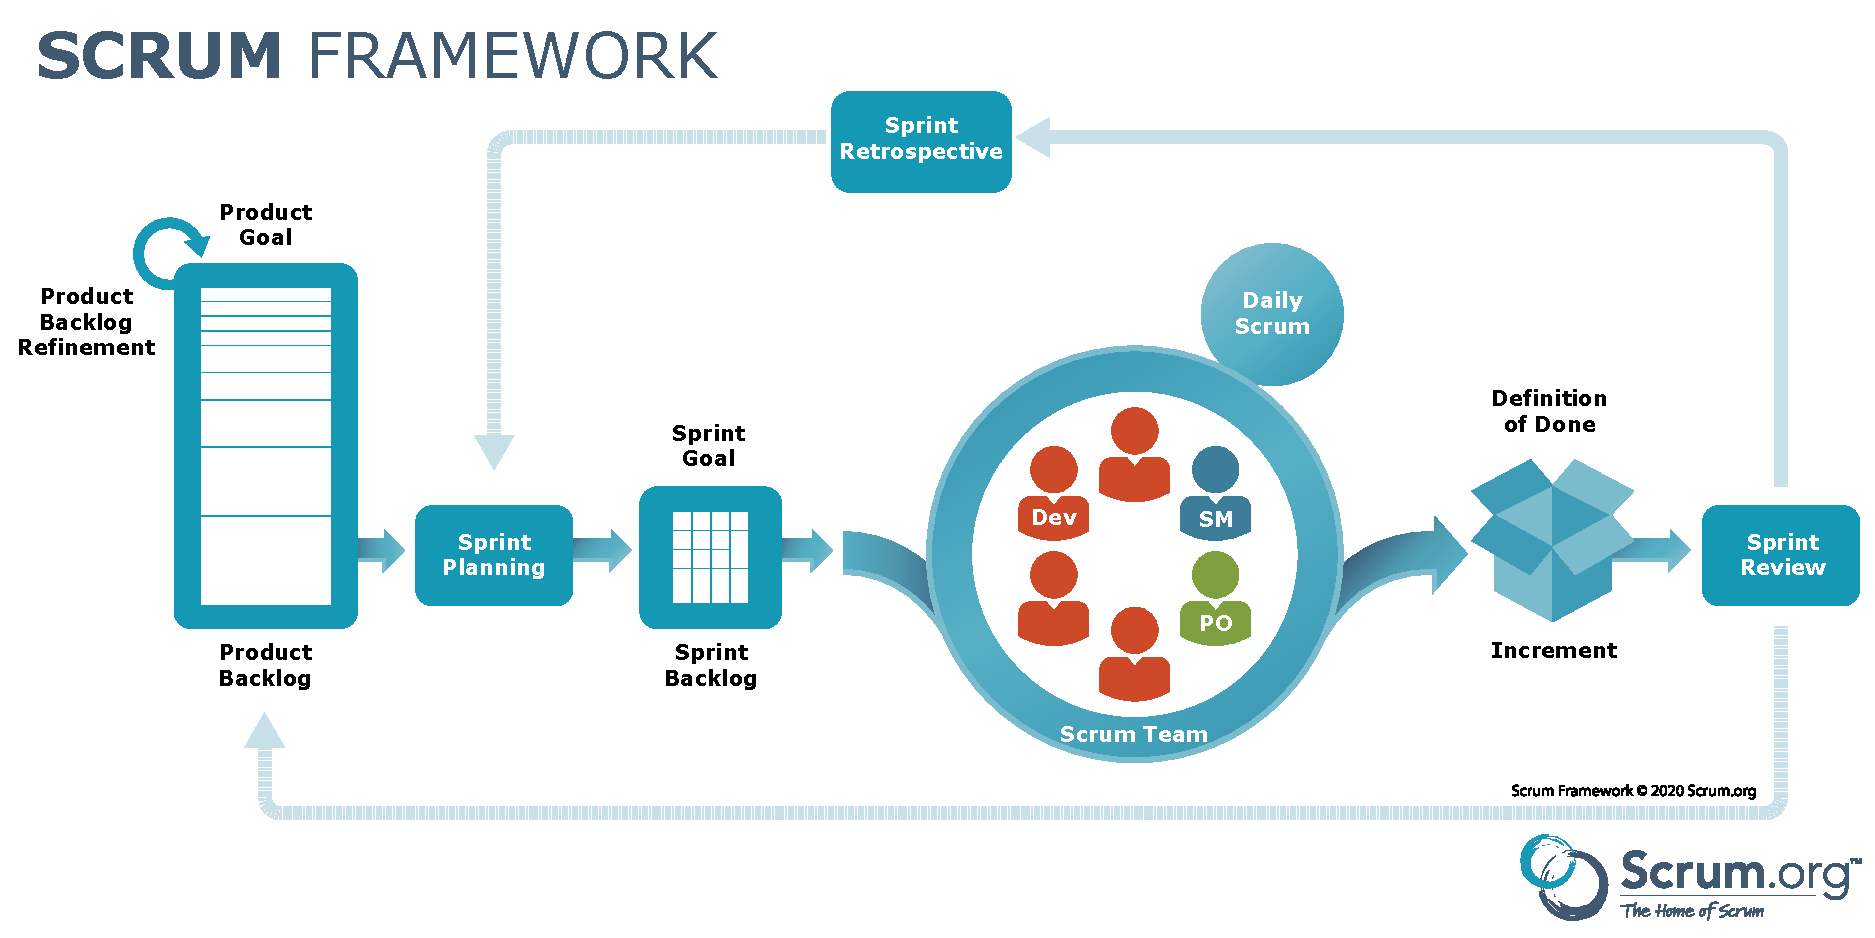
\includegraphics[width=\textwidth]{imaxes/scrum.pdf}
  \caption{Diagrama de la metodología \textit{Scrum} \citep{scrumorg}.}
  \label{fig:scrum}
\end{figure}

Scrum se basa en la teoría del control empírico de procesos, o empirismo. Esta sostiene que el conocimiento proviene de la experiencia y de tomar decisiones basadas en lo que se sabe. Este marco de trabajo propone un enfoque iterativo e incremental para mejorar la predictibilidad y controlar el riesgo. Tres pilares respaldan cada implementación del control empírico de procesos: transparencia, inspección y adaptación.

\begin{itemize}
    \item \textbf{Transparencia}: Aspectos significativos del proceso deben ser visibles para quienes son responsables del resultado. La transparencia requiere que esos aspectos estén definidos por unos estándares comunes para que los responsables tengan un entendimiento acorde acerca de estos resultados.
    \item \textbf{Inspección}: Los usuarios de Scrum deben revisar con frecuencia los artefactos de Scrum y el progreso hacia un objetivo común para detectar desviaciones no deseadas.
    \item \textbf{Adaptación}: Si durante la inspección del trabajo un miembro del equipo determina que ha habido desviaciones significativas con respecto a los objetivos iniciales el proceso y las tareas deben adaptarse lo antes posible con el objetivo de reducir o eliminar esta desviación.
\end{itemize}

\subsubsection{Roles}

Un equipo de Scrum debe ser auto-organizativo y multifuncional: el equipo debe ser capaz de dirigirse a sí mismo y debe poseer las competencias necesarias para la consecución del trabajo sin dependencias externas. Para ello se definen los siguientes roles:

\begin{itemize}
    \item \textit{Product Owner}: este es responsable de maximizar el valor del producto resultado del trabajo del \textit{equipo de desarrollo}. La forma en que esto se consiga puede variar de un equipo a otro.
    
    \item \textit{Equipo de desarrollo}: este esta formado por profesionales que se encargan de la realización del producto <<Terminado>> después de cada incremento, el cual constituye los resultados del mismo.
    
    \item \textit{Scrum master}: este es responsable de promover y apoyar que se siguen las pautas correctas de realización del Scrum en el proyecto. Debe ayudar a que el equipo entienda los conceptos de scrum para poder maximizar el valor entregado.
    
\end{itemize}

\subsubsection{Eventos}

Además de los roles anteriores existen una serie de eventos pre-establecidos con una duración predeterminada. Estos tienen como finalidad la establecer una regularidad en el proyecto de forma que se minimicen las reuniones no establecidas por scrum. Estos eventos son:

\begin{itemize}

    \item \textit{Sprint}: constituye un incremento o iteración del producto. Tiene una duración generalmente de entre 2-4 semanas en el que se desarrolla una parte del producto. Durante el \textit{sprint}, el equipo se compromete a entregar un conjunto específico de funcionalidades.
    \item \textit{Sprint planning}: la planificación del \textit{sprint} es una reunión entre el todos los miembros del equipo, donde se define de forma colaborativa el trabajo que se llevará a cabo durante el mismo. Tiene una reunión máxima de ocho horas, aunque suele ser menor según la duración del \textit{sprint}.
    \item \textit{Daily scrum}: se trata de una breve reunión (máximo 15 minutos) donde el equipo de trabajo planifica las tareas que se llevarán a cabo durante el día. Además, se realiza una inspección para verificar que el equipo progrese adecuadamente hacia los objetivos marcados.
    \item \textit{Sprint review}: esta reunión de carácter más informal se da al final de cada \textit{sprint}. En ella el equipo completo (junto a \textit{stakeholders}\footnote{Aquellos interesados en la realización del proyecto.}) realiza la inspección del incremento demostrando los resultados del \textit{sprint} y añadiendo al \textit{product backlog} aquellas funcionalidades <<terminadas>>.
    \item \textit{Sprint retrospective}: reunión de carácter más filosófico que se da entre el \textit{Sprint review} y el próximo \textit{Srint planning} donde el equipo <<se inspecciona a sí mismo>>: se comparten impresiones acerca del incremento, reflexionando acerca de aquellos aspectos del proceso que han ido bien y aquellos que son sujetos de mejora.

\end{itemize}

\subsubsection{Artefactos}

Los artefactos de Scrum representan valor o trabajo diseñados para mejorar la transparencia y facilitar la inspección del proyecto. Esto artefactos son los siguientes:

\begin{itemize}
    \item \textit{Product backlog}: esta es una lista ordenada de todas aquellas funcionalidades y tareas que serán necesarias en el producto. Este representa los requisitos deseado del producto. Esta nunca está del todo completa: evoluciona a lo largo del tiempo con el producto a medida que los requisitos cambian o se entienden mejor.
    \item \textit{Sprint backlog}: conforma el conjunto de elementos del \textit{Product backlog} escogidos para su realización en el marco de un \textit{Sprint}. Este incluye el plan diseñado para la entrega de incremento en cuestión y la realización del objetivo del mismo.
\end{itemize}

\subsection{Adaptaciones de \textit{Scrum} al proyecto}
\label{subsec:adaptaciones-scrum}

Varios factores como la presencia de un único miembro en el equipo de desarrollo, la falta de regularidad en la dedicación del mismo debido a obligaciones académicas han impedido que se haya podido llevar a cabo la metodología seleccionada de forma totalmente fiel a sus pautas. Por un lado se ha realizado la siguiente asignación de roles:

\begin{itemize}
    \item El rol de \textit{Product owner} ha sido desempeñado por el alumno Nicolás Míguez García.
    \item El rol de \textit{Scrum master} ha sido desempeñado por los directores de este proyecto Patricia Martín Rodilla y David Otero Freijeiro.
    \item El de equipo de trabajo estuvo constituido por un único miembro, el alumno Nicolás Míguez García.
\end{itemize}

A continuación, se presentan las modificaciones implementadas en la metodología original para adecuarla a las necesidades de este proyecto

\begin{itemize}
    \item Aunque debido a las obligaciones académicas del alumno, en ocasiones, no se ha podido mantener la continuidad entre \textit{sprints}, sí que se ha intentado mantener constante su duración en aproximadamente 3 semanas.
    \item Al contrario que la duración, la carga de trabajo en cada \textit{sprint} ha ido variando, en función de la dedicación disponible por parte del equipo de desarrollo. En general los primeros \textit{sprints} son los más livianos y los últimos los que mayor carga de trabajo tienen.
    \item Dado que el equipo de desarrollo está compuesto por una sola persona, el evento de \textit{Daily scrum} pierde el sentido de su existencia. Sin embargo, se mantiene la práctica de la revisión del trabajo diario como parte de las responsabilidades del alumno.
\end{itemize}

\subsubsection{Elementos del \textit{Backlog}}
Para definir los elementos del \textit{Product backlog} (y por tanto los requisitos funcionales del proyecto) se han usado las \textbf{historias de usuario}. Estas constituyen una técnica muy utilizada en metodologías ágiles para la especificación de requisitos debido a su sencillez y claridad. Estas se tratan descripciones breves (una o dos líneas) de las funciones del sistema desde la perspectiva del usuario. Las historias de usuario tienen de la siguiente forma:

\begin{center}
     \textit{Como <rol> quiero <algo> para poder <beneficio>.}
\end{center}
%Para medir el esfuerzo necesario para completar una historia de usuario, se emplean puntos de historia. Estos puntos reflejan el nivel de esfuerzo teniendo en cuenta varios factores, como la cantidad de trabajo, la complejidad del mismo o el riesgo asociado.

Por otro lado, debido a que la primera fase del proyecto estaba más orientada hacia la investigación y desarrollo de los algoritmos de perfilado automático que al desarrollo de un producto software en sí mismo, el modelado de requisitos desde la perspectiva de usuario no tiene demasiado sentido. Es por ello que los requisitos de esta fase se modelan como \textbf{tareas técnicas} orientadas al desarrollador en vez de al usuario. Estas se pueden ver como parte de una gran historia de usuario inicial, denominada \textbf{épica}, que dura varios incrementos la cual se menciona en el capítulo~\ref{chap:analisis}.% No obstante, por ser uniformes en todo el proyecto el esfuerzo en estas tareas técnicas se modelará igualmente mediante puntos de historia.

\section{Gestión del proyecto}
La gestión del proyecto se encarga de la planificación, seguimiento y control del mismo, teniendo en cuenta factores como la estimación y la asignación y control de recursos. Esto proporciona una visión global acerca del estado del proyecto en cualquier momento de su desarrollo.
\subsection{Estimación y planificación}
Como se comentó en la sección~\ref{subsec:adaptaciones-scrum}, la duración de un \textit{sprint} se ha intentado mantener constante en 3 semanas. Cada \textit{sprint} se ha estimado en 45 horas de trabajo, lo que corresponden a 3 horas al día sin contar fines de semana.

No obstante, debido a las obligaciones académicas y laborales del alumno, la cantidad de esfuerzo diario y entre \textit{sprints} ha ido variando. De esta forma, en general los primeros \textit{sprints} han tenido una menor carga de trabajo mientras que la de los últimos ha sido mayor. Sin embargo, las horas de trabajo por \textit{sprint} en promedio se puede decir que se han mantenido de acuerdo a la estimación inicial.

En el proyecto finalmente se han planificado los siguientes \textit{sprints}:
\begin{itemize}
    \item \textbf{Sprint 1}: Configuración del entorno e investigación del estado del arte (14-3-2023 a 4-4-2023)
    \item \textbf{Sprint 2}: Búsqueda, comparación y selección de algoritmos y \textit{datasets} a usar (4-3-2023 a 25-4-2023)
    \item \textbf{Sprint 3}: Adaptación de algoritmo de \citet{loscalis22} y creación de \textit{scraper} para descarga de \textit{dataset} (25-4-2023 a 16-5-2023)
    \item \textbf{Sprint 4}: Adaptación de algoritmos restantes y extracción de resultados (20-6-2023 a 11-7-2023)
    \item \textbf{Sprint 5}: Desarrollo del micro-servicio de perfilado (11-7-2023 a 1-8-2023)
    \item \textbf{Sprint 6}: Inicio del «frontend» y creación de las primeras visualizaciones (1-8-2023 a 21-8-2023)
    \item \textbf{Sprint 7}: Lista y detalle de usuarios (21-8-2023 a 11-9-2023)
    \item \textbf{Sprint 8}: Persistencia de las colecciones y rediseño del «Dashboard» (11-9-2023 a 2-10-2023)
    \item \textbf{Sprint 9}: Lista de colecciones y filtrado de usuarios por categoría (2-9-2023 a 23-10-2023)
    %\item Sprint 10: Redacción de la memoria (23-10-2023 6-11-2023)
\end{itemize}

\subsection{Recursos}
Para empezar, los recursos humanos asignados ha este proyecto son los que se mencionan en el apartado~\ref{subsec:adaptaciones-scrum}, que conforman:

\begin{itemize}
    \item Los directores del proyecto: Patricia Martín Rodilla y David Otero Freijeiro.
    \item El alumno: Nicolás Míguez García.
\end{itemize}

En cuanto a los recursos materiales empleados únicamente está el equipo personal del alumno: un portátil \textit{Lenovo ThinkPad X260} 12" Core i5 2.4 GHz - SSD 256 GB - 8GB de memoria RAM valorado en \textbf{428€}. Por otra parte, los recursos de tipo software utilizados son todos gratuitos.

\subsection{Costes}
Para el cálculo de los costes totales del proyecto, se ha tenido en cuenta la Guía salarial de \citet{hays2022}. Según la media de varias ciudades en España, para un desarrollador Python se ha obtenido un sueldo de 33.400€ aproximadamente. Mientras que, una media de 57.200€ anuales para un \textit{Project Manager}. Si calculamos el coste por hora de ambos teniendo en cuenta 1.820 horas de trabajo al año, nos sale, aproximando, \textbf{18€/h} para desarrollador Python y \textbf{31€/h} para un \textit{Project Manager}. Teniendo en cuenta estos salarios, en la tabla~\ref{tab:metodologia/costes} podemos ver el cálculo final del coste del proyecto.

\begin{table}[H]
    \centering
    \rowcolors{2}{white}{udcgray!25}
    {
    \setlength{\tabcolsep}{1\tabcolsep}
    \begin{tabular}{|c|c|c|c|}
        \hline
        \rowcolor{udcpink!25}
        \textbf{Rol} & \textbf{Coste/hora} & \textbf{Tiempo de trabajo} & \textbf{Total} \\ \hline
        Equipo & 18€ & 45h x 9 \textit{sprints} & 7.290 € \\ \hline
        \textit{Project Managers} & 31€ & 2 x 1.5h x 9 \textit{sprints} & 837 € \\ \hline
        Material & -- & -- & 428 € \\ \hline
        \textbf{Total} & -- & -- & \textbf{8.555 €} \\ \hline

    \end{tabular}%
    }
    \caption{Tabla con el cálculo de costes final para el proyecto.}
    \label{tab:metodologia/costes}
\end{table}
 \chapter{Análisis de requisitos}
\label{chap:analisis}
En este capítulo se muestra el análisis de requisitos efectuado para el desarrollo del dashboard web.

\section{Requisitos funcionales}
Como ya se ha mencionando en el capítulo \ref{chap:metodologia} se han usado las historias de usuarios como técnica de especificación de las funcionalidades que debe cubrir el producto. A continuación en la tabla \ref{tab:user-stories} se muestran las historias de usuario extraídas.
\begin{table}[H]
{
    \setlength\arrayrulewidth{0.75pt}
    \setlength{\tabcolsep}{0.9\tabcolsep}

    \begin{tabular}{|p{0.04\linewidth} | p{0.78\linewidth}|}
    \hline
    Id & Historia de usuario \\ \hline
    H1 & \textbf{Como} usuario \textbf{quiero} perfilar el género y edad de los usuarios de una colección \\ \hline
    H4 & \textbf{Como} usuario \textbf{quiero} ver las estadísticas de edad en forma de gráfico de los usuarios perfilados en una colección \\ \hline
    H7 & \textbf{Como} usuario \textbf{quiero} ver las estadísticas de género en forma de gráfico de los usuarios perfilados en una colección \\ \hline
    H5 & \textbf{Como} usuario \textbf{quiero} ver estadísticas propias de la colección perfilada como nombre, tiempo, algoritmo y usuarios totales de la misma \\ \hline
    H2 & \textbf{Como} usuario \textbf{quiero} elegir entre los distintos algoritmos de perfilado disponibles \textbf{para} ver las diferencias entre las predicciones de cada uno de ellos \\ \hline
    H3 & \textbf{Como} usuario \textbf{quiero} ver la lista de usuarios perfilados con su información asociada \\ \hline

    H6 & \textbf{Como} usuario \textbf{quiero} ver las publicaciones de un usuario específico de la colección junto a sus datos demográficos \textbf{para} comparar el tipo de redacción y temáticas tratadas según los grupos demográficos predichos \\ \hline

    H8 & \textbf{Como} usuario \textbf{quiero} guardar las colecciones previamente perfiladas \textbf{para} acceder a ellas sin necesidad de volver a perfilarlas de nuevo \\ \hline
    H9 & \textbf{Como} usuario \textbf{quiero} ver una lista ordenada temporalmente que incluya datos generales de las colecciones previamente perfiladas \textbf{para} buscar entre ellas con facilidad \\ \hline
    \end{tabular}%
}
    \caption{Requisitos funcionales de la aplicación.}
\label{tab:user-stories}
\end{table}

\section{Requisitos no funcionales}
Los requisitos no funcionales, por otro lado, no se ven reflejados en funcionalidades independientes que satisfacen necesidades específicas de una aplicación. Sino que, estos constituyen requerimientos generales sobre cómo debería comportarse el sistema de forma global y están relacionados con la operatividad y calidad software. En nuestro sistema se ha priorizado nuestra atención en los enumerados en la tabla \ref{tab:rnf}.

\begin{table}[H]
{
    \setlength{\tabcolsep}{0.4\tabcolsep}
    
    \begin{tabular}{|p{0.07\linewidth} | p{0.17\linewidth}| p{0.63\linewidth}|}
    \hline
    Id & Nombre & Descripción\\ \hline
    RNF-1 & Usabilidad & La aplicación debe tener un interfaz intuitiva y familiar con el usuario permitiendo una interacción lo más eficiente posible.\\ \hline
    RNF-2 & Mantenibilidad & La aplicación debe ser diseñada de forma legible y modular con el objetivo de permitir extender fácilmente su funcionalidad.\\ \hline
    % RNF-3 & Escalabilidad & El sistema debe ser capaz de aumentar la carga de trabajo bajo demanda. \\ \hline
    RNF-3 & Fiabilidad & El sistema debe ser confiable y consistente, siendo tolerante a fallos. \\ \hline
    RNF-4 & Portabilidad & La aplicación debe ser capaz de ejecutarse en distintos entornos sin modificaciones significativas.\\ \hline
    RNF-5 & Escalabilidad & El sistema debe ser fácilmente escalable ante el crecimiento de la carga de trabajo debido a un aumento de la demanda.\\ \hline
    \end{tabular}%
}
    \caption{Requisitos no funcionales detectados.}
\label{tab:rnf}
\end{table}

\section{Modelo de datos}
Como parte del análisis del dominio se realizó un diagrama entidad-relación, para conocer las entidades relevantes de nuestro sistema y enfocar de manera clara el diseño de la base de datos. No obstante, aunque las entidades principales del mismo se han mantenido, debido al enfoque incremental del proyecto, a medida que ha ido avanzando estas han estado sujetas a cambios. Por lo que en la figura \ref{fig:diagrama/ER} se muestra el diagrama entidad-relación al finalizar el proyecto.

\begin{figure}
  \centering
  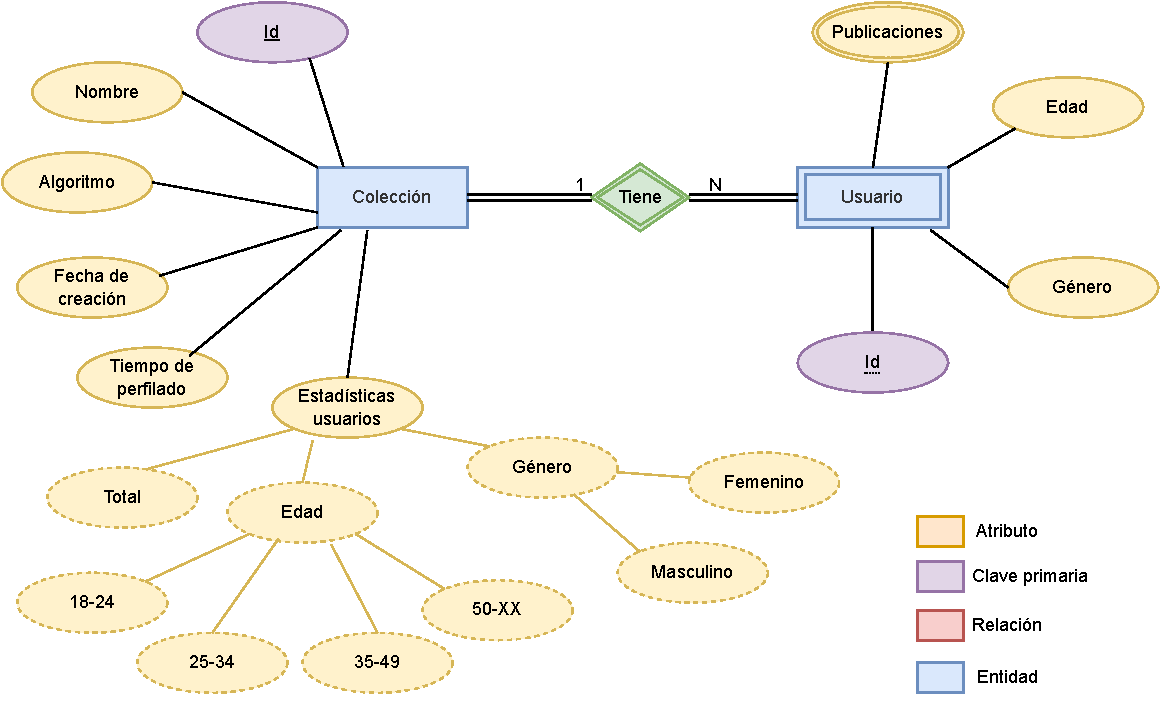
\includegraphics[width=\textwidth]{imaxes/diagramas/ER-diagram.pdf}
  \caption{Diagrama de entidad-relación del sistema.}
  \label{fig:diagrama/ER}
\end{figure}

Como se puede observar se tienen únicamente dos entidades fundamentales relacionadas entre sí: \textit{Colección} y \textit{Usuario}. 
% \begin{itemize}
%     \item \textbf{\textit{Colección}}: esta entidad representa una colección de usuarios ya perfilada
% \end{itemize}
 \chapter{Diseño}
\label{chap:design}
\section{Prototipado}
\label{sec:prototipo}
\lettrine{E}{l} prototipo de una aplicación conforma una versión inicial <<hueca>> de un producto. Es una herramienta fundamental para visualizar conceptos de diseño, funcionalidad e interacción con el usuario en una etapa temprana de desarrollo. Permite una comunicación efectiva entre el equipo de desarrollo y el cliente, haciendo posible la identificación de problemas antes de la implementación del producto, donde un cambio de requisitos es poco costoso, garantizando que la aplicación satisfaga las necesidades y expectativas de los usuarios finales.

En nuestro caso, como técnica de prototipado hemos optado por utilizar \textit{wireframes}. Los \textit{wireframes} son una herramienta de prototipado basados en representaciones visuales simplificadas de la interfaz de una aplicación. En estos se plasma la estructura y disposición de los elementos fundamentales de la aplicación sin añadir detalles decorativos como elementos de diseño gráfico o colores, centrándose en la funcionalidad y navegación de la misma.

En la figura \ref{fig:proto-home} se puede ver el diseño de la página principal de nuestra interfaz. Como vemos en ella se expone la funcionalidad principal de perfilar una colección de usuarios, a partir de un archivo. Esta página, está formada por un formulario donde se puede seleccionar el algoritmo de perfilado junto con el fichero que contiene la colección a perfilar. Por otro lado, también tiene una barra de navegación en la parte de arriba que se mantendrá para el resto de \textit{wireframes} de la aplicación.

\begin{figure}[H]
  \centering
  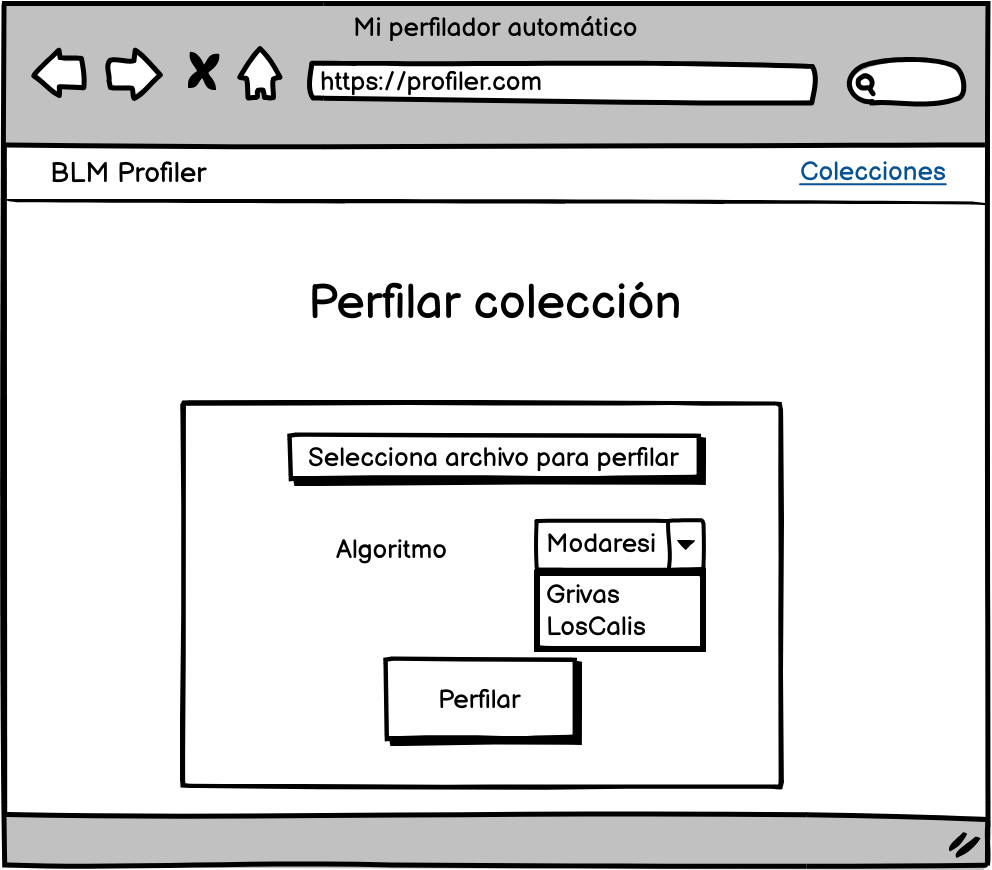
\includegraphics[width=\textwidth]{imaxes/prototipo/home.png}
  \caption{Prototipo de la página principal de la aplicación.}
  \label{fig:proto-home}
\end{figure}

En el caso de seleccionar el enlace <<Colecciones>>, de la barra de navegación, nos iríamos a una página como la de la figura \ref{fig:proto-collections}. En esta se muestra una tabla, ordenada temporalmente, con todas las colecciones de usuarios previamente perfilados de nuestra aplicación, junto a información general sobre cada una como: algoritmo, usuarios totales o fecha de perfilado.

\begin{figure}[H]
  \centering
  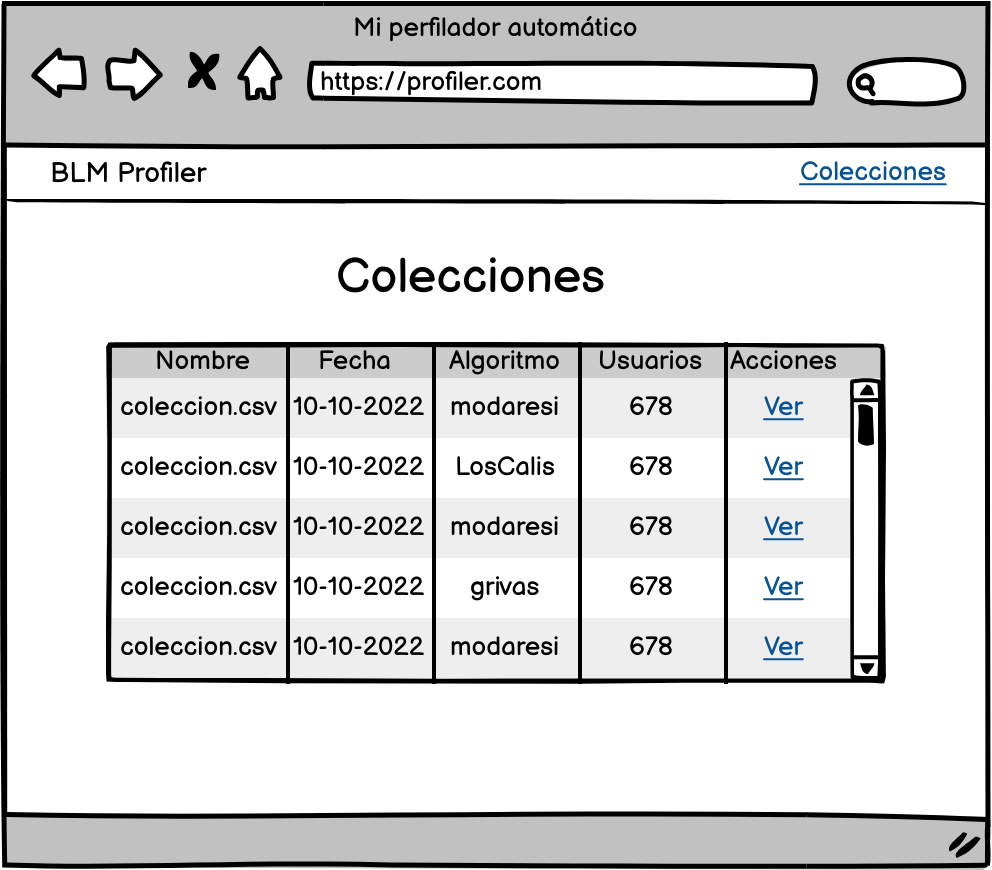
\includegraphics[width=\textwidth]{imaxes/prototipo/collections.png}
  \caption{Prototipo de ver colecciones perfiladas.}
  \label{fig:proto-collections}
\end{figure}

En el caso de seleccionar <<Ver>> una colección de la lista de colecciones (\ref{fig:proto-collections}) o tras perfilar una nueva en la página principal (\ref{fig:proto-home}) nos iríamos a la visualización del \textit{dashboard} o cuadro de mando de la colección (\ref{fig:proto-dashboard}). En este \textit{wireframe} se muestran dos gráficas sobre los datos demográficos, edad y género en este caso, de los usuarios perfilados. Además también se muestra una tabla con la lista de usuarios de la colección junto con las predicciones realizadas sobre cada uno y un enlace sobre una muestra de una publicación del mismo. Por otro lado, en la parte de arriba tenemos unos desplegables que nos permiten filtrar los datos de la tabla y gráficas según la categoría elegida; junto con unas tarjetas en las que se muestran detalles generales de la colección.

\begin{figure}[H]
  \centering
  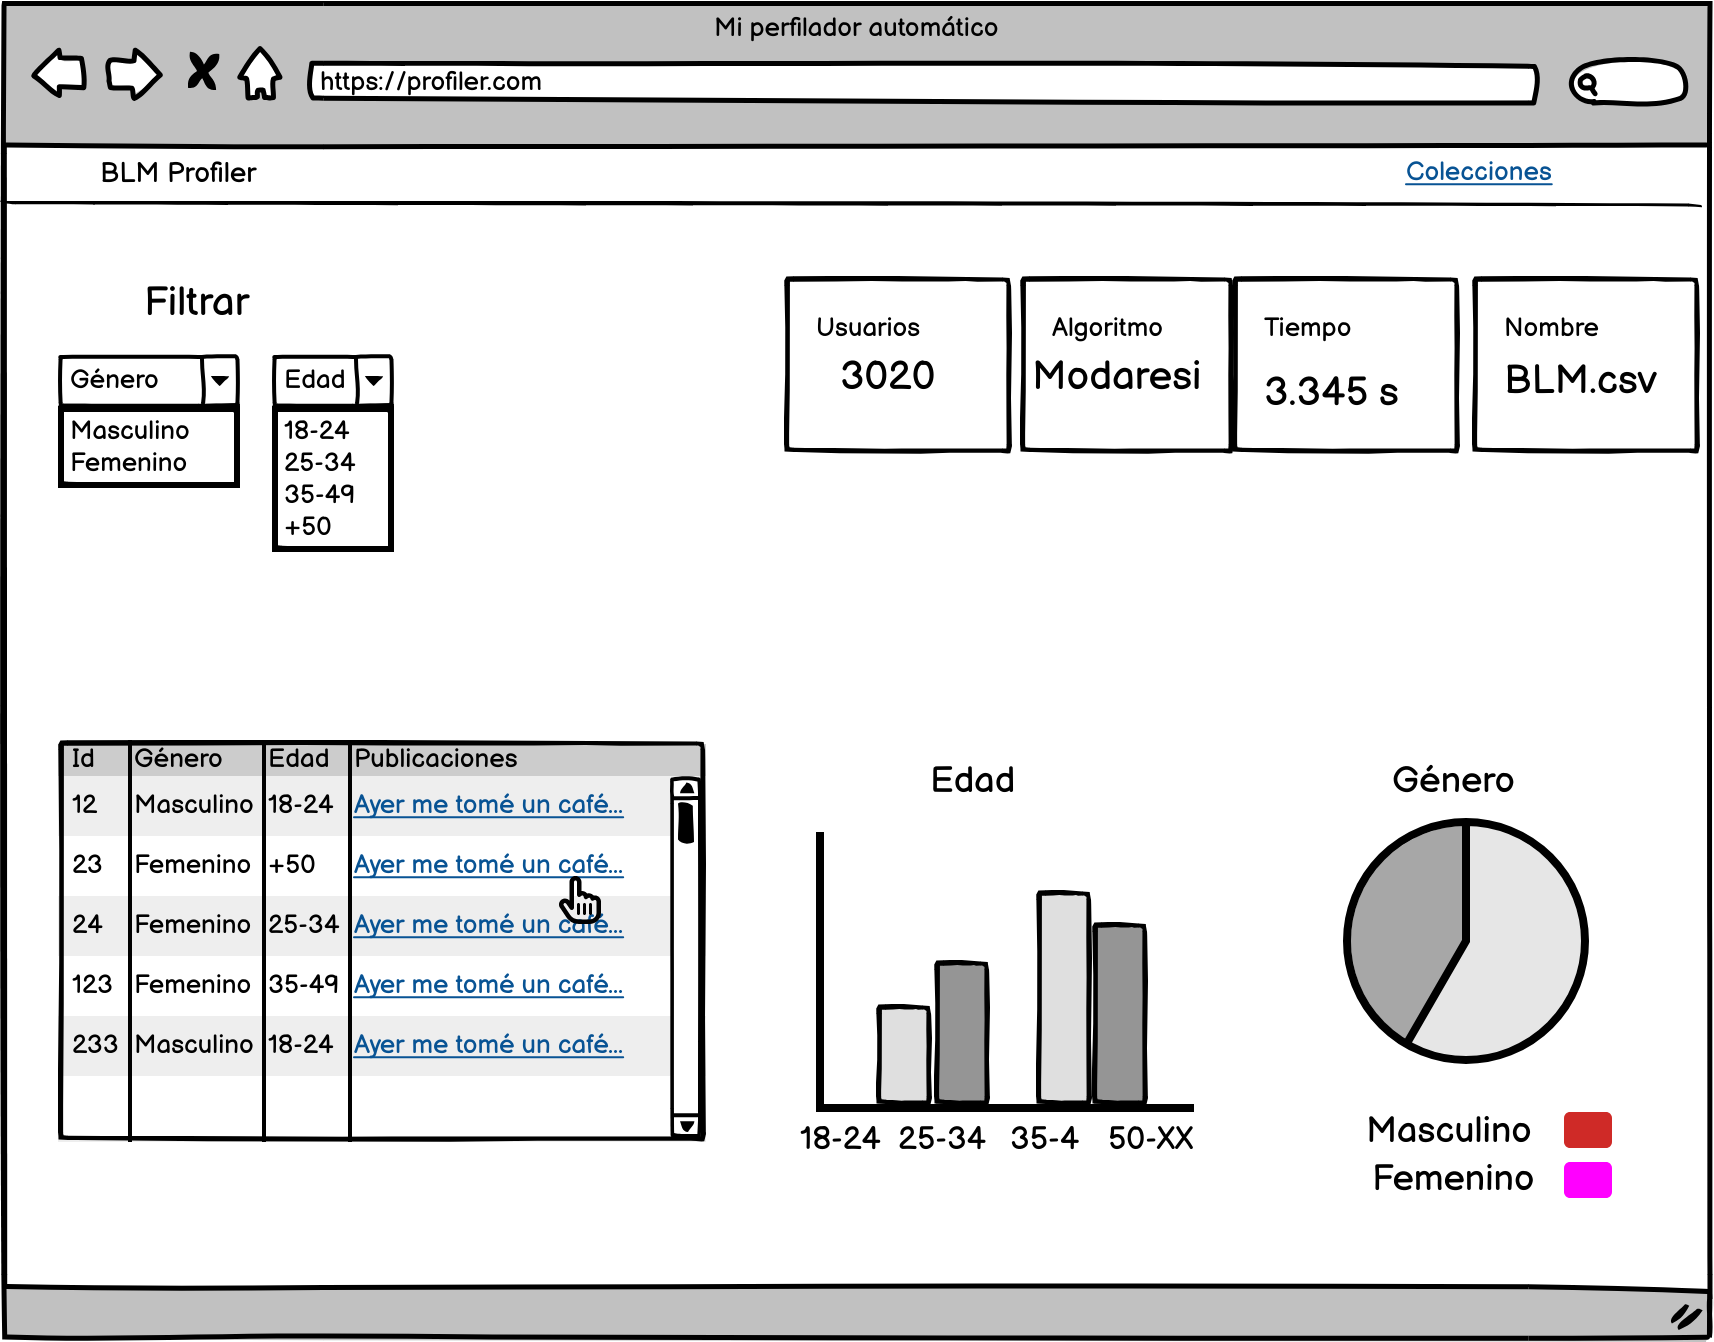
\includegraphics[width=\textwidth]{imaxes/prototipo/dashboard-unfiltered.png}
  \caption{Prototipo del cuadro de mando de la aplicación.}
  \label{fig:proto-dashboard}
\end{figure}

En el caso de seleccionar algún filtro en el \textit{dashboard} se añadiría al mismo una lista, como la de la figura \ref{fig:proto-dashboard-filtered}, con aquellos seleccionados donde se podrían quitar de nuevo estos. Y se mostrarían las modificaciones en los gráficos y lista.

\begin{figure}[H]
  \centering
  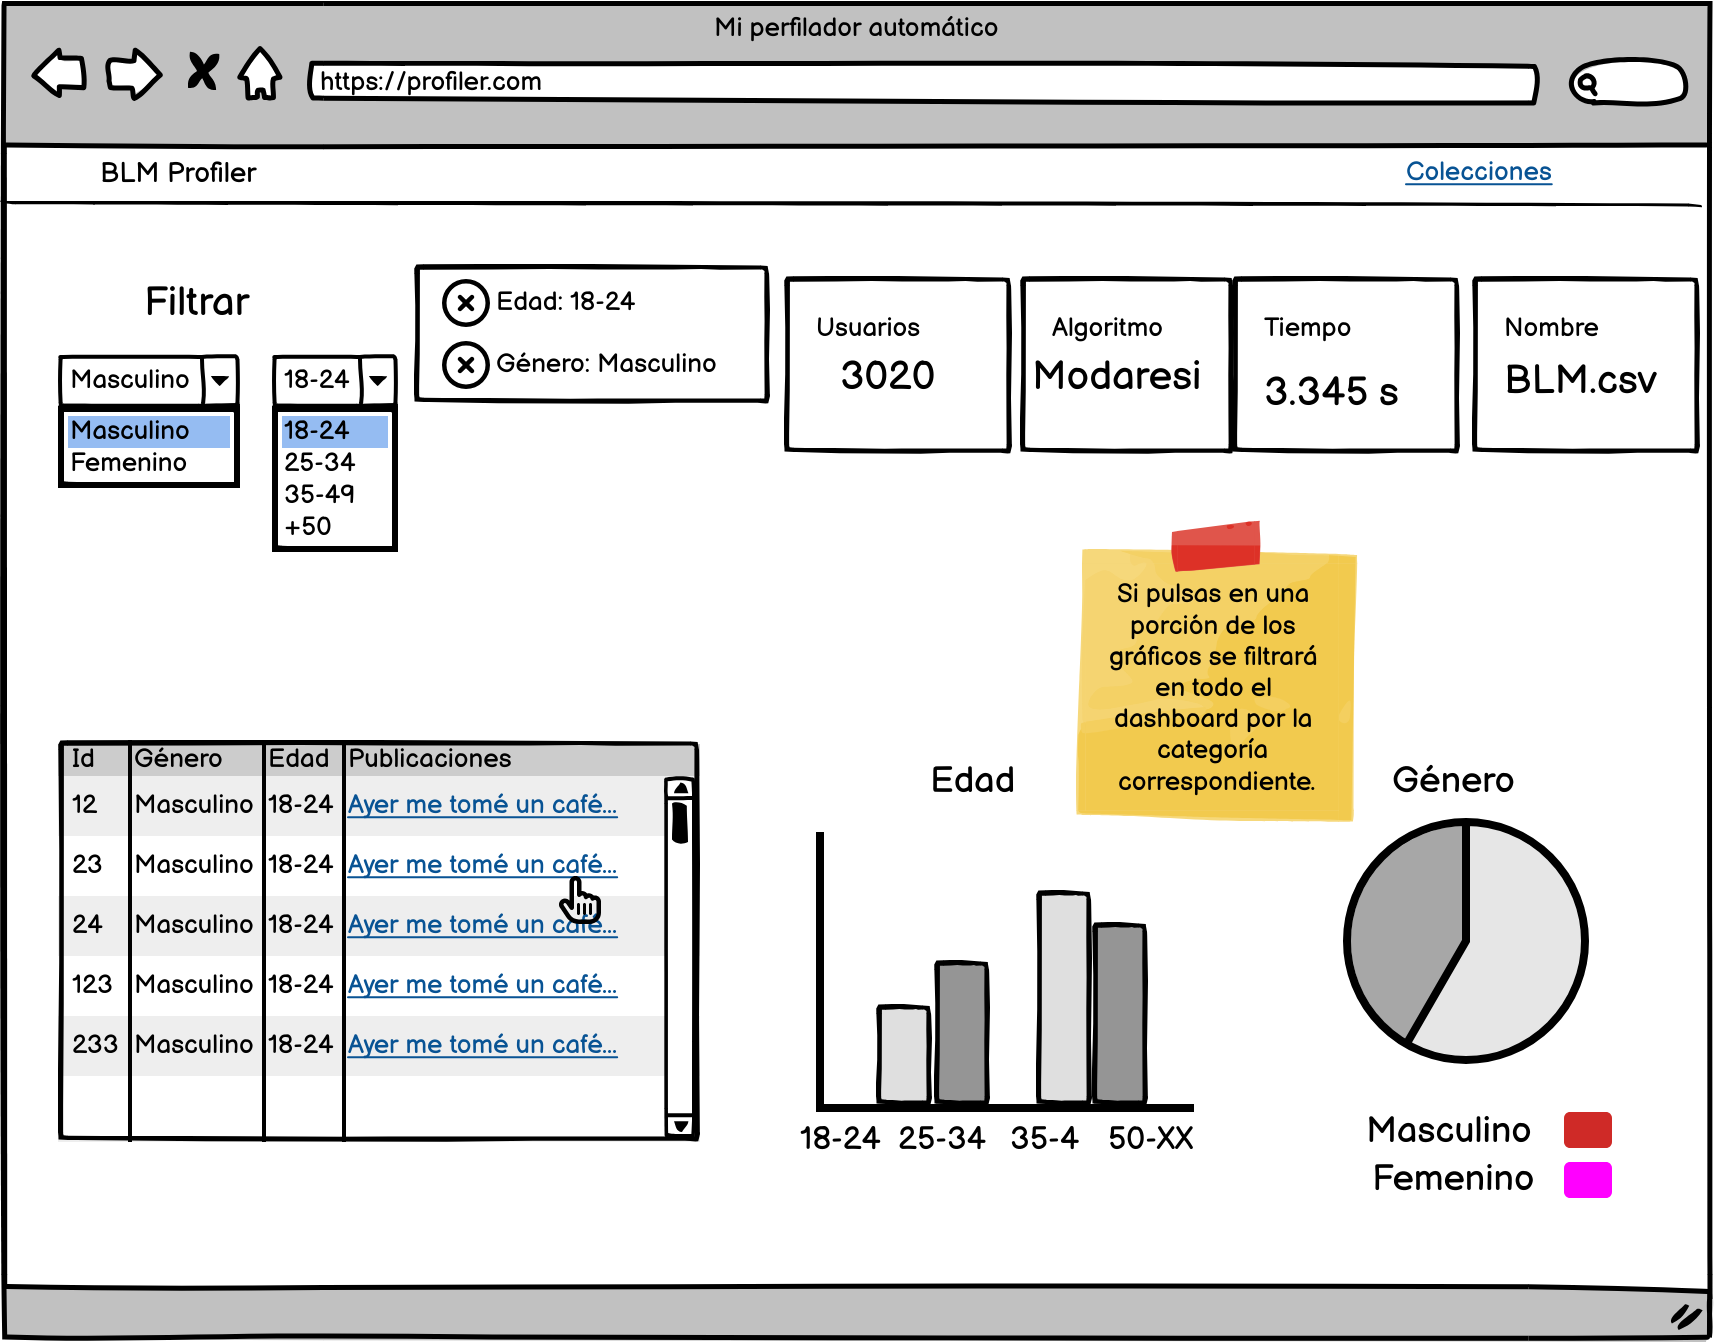
\includegraphics[width=\textwidth]{imaxes/prototipo/dashboard-filtered.png}
  \caption{Prototipo del cuadro de mando al especificar filtros sobre edad y género.}
  \label{fig:proto-dashboard-filtered}
\end{figure}

Por último, al seleccionar el enlace de la publicación de un usuario del \textit{dashboard}, se navegaría hasta la última página de nuestra web, donde se podría ver en detalle las publicaciones del usuario seleccionado junto con sus datos generales. Además, esta tendría un botón para volver al \textit{dashboard} de la colección. En el \textit{wireframe} de la figura \ref{fig:proto-info-user} se muestra la disposición de la misma.

\begin{figure}[H]
  \centering
  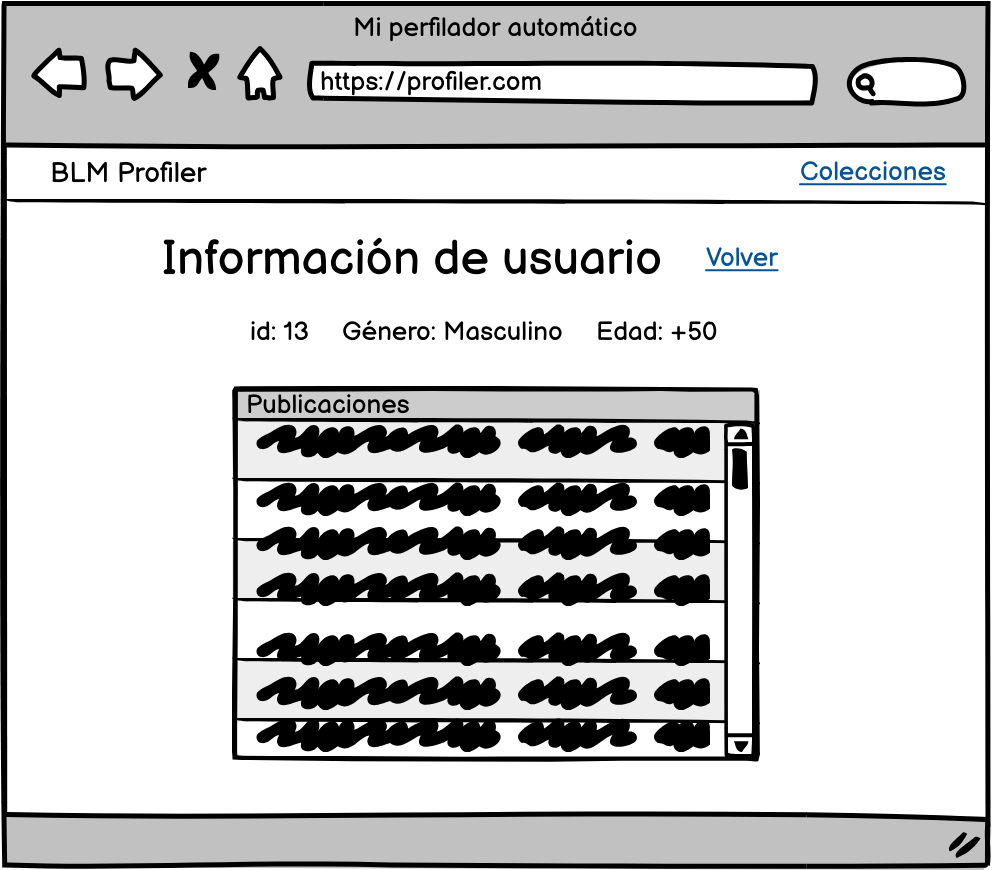
\includegraphics[width=\textwidth]{imaxes/prototipo/info-user.png}
  \caption{Prototipo de ver información de usuario en detalle.}  \label{fig:proto-info-user}
\end{figure}

\section{Arquitectura}
\label{sec:arquitectura}
El diseño de la arquitectura de una aplicación es un aspecto de vital importancia para cumplir con los requisitos tanto funcionales como no funcionales de la misma. Dada la naturaleza ágil de la metodología seguida, la arquitectura del sistema ha ido evolucionando durante el desarrollo del mismo, pasando de un diseño más sencillo a uno más complejo. Por este motivo, en este apartado se describirá el diseño final de la arquitectura propuesta.

En nuestro caso, como se puede ver en la figura \ref{fig:diagrama/arquitectura} hemos seguido una arquitectura cliente-servidor distribuida o en n-capas, donde el servidor está dividido en servidor web, servidor de aplicación y servidor de datos. El servidor web es el que aloja la aplicación web SPA, que su vez está divido en interfaz de usuarios y capa de acceso a servicios. El servidor de aplicación se encarga de exponer la API REST que ejecuta la lógica de negocio de la aplicación y el acceso a datos\footnote{Y de comunicarse con el micro-servicio de perfilado como se comenta más adelante.}. Por último, el servidor de datos es el encargado de almacenar los datos de la aplicación. 

\begin{figure}[H]
  \centering
  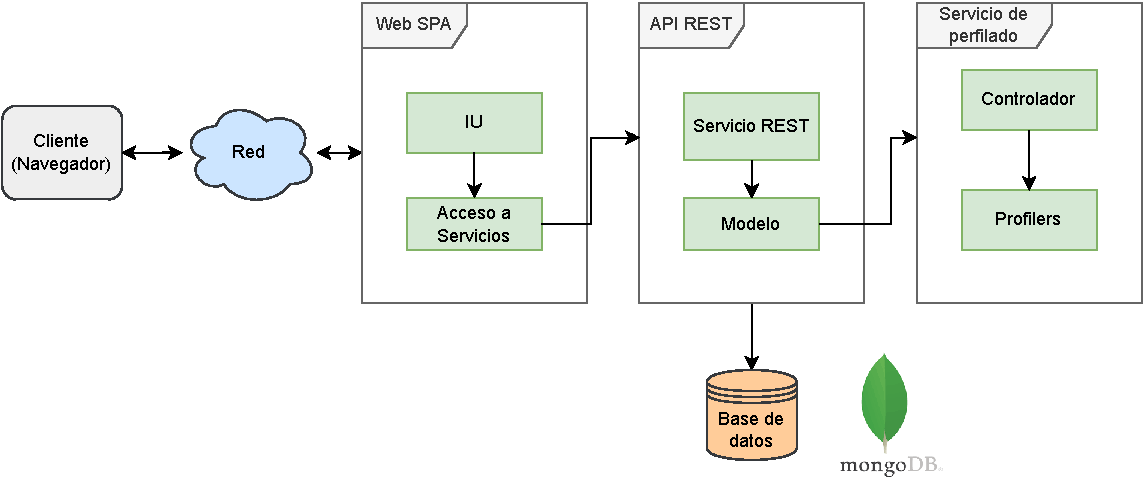
\includegraphics[width=\textwidth]{imaxes/diagramas/arquitectura.pdf}
  \caption{Diagrama de la arquitectura global del sistema.}  \label{fig:diagrama/arquitectura}
\end{figure}

Además se puede ver que existe un servidor adicional, que se podría definir como un micro-servicio, cuya única funcionalidad es la de ejecutar los algoritmos de perfilado sobre los datos de usuarios que le envíe la API REST y devolver estos perfilados. Por lo tanto, la el servidor de la aplicación también actúa como cliente de este servicio. \footnote{La decisión de separar este servicio del resto del \textit{backend} se tomó inicialmente debido a la dificultad de hacer la migración de los algoritmos existentes a una versión actual de Python como se comentará en el capítulo de desarrollo, sin embargo, este enfoque tiene otros beneficios importantes que se comentan a continuación.}

La decisión de tener esta arquitectura distribuida en varias capas tiene varias ventajas:
\begin{itemize}
    \item Para empezar, se favorece la escalabilidad del sistema (\hyperref[tab:rnf]{RNF-5}). El hecho de tener servidores distintos para \textit{frontend}, \textit{backend} y el micro-servicio de perfilado permite que se puedan escalar horizontalmente estos de forma selectiva. Esto es importante porque el micro-servicio de perfilado representa la carga más significativa del sistema en cuanto a recursos computacionales y tiempo, lo que la convierte en un posible cuello de botella para el funcionamiento general del mismo. Por otra parte, el servidor web es el que menos recursos computacionales consume.
    \item Por otro lado, se favorece la mantenibilidad y extensibilidad del software (\hyperref[tab:rnf]{RNF-2}). Al tener las distintas capas separadas, se posibilita el poder extender o reemplazar cualquiera de ellas sin necesidad de hacer un cambio en las demás\footnote{Este hecho se alinea con unas buenas prácticas de ingeniería, cumpliendo con un principio de diseño fundamental como es el abierto-cerrado.}. Un ejemplo de esto sería añadir un cliente móvil además del web, añadir otra API que consumiera el micro-servicio de perfilado, o incluso extender este último para dar soporte a nuevos algoritmos o mejoras de rendimiento. De igual forma, esta separación nos permite elegir el lenguaje de programación o tecnología más adecuada para la implementación de cada capa.
    \item Por último, otra ventaja de este enfoque sería el aumento de fiabilidad del mismo (\hyperref[tab:rnf]{RNF-3}). El fallo en cualquier capa no implica que el resto no puedan seguir funcionando.
\end{itemize}

\subsection{\textit{Backend}}

Como ya se ha comentado, el \textit{backend} está dividido en dos capas: servicios y modelo que a su vez se podría dividir en lógica de negocio y acceso a datos. Para la implementación de estas capas se han seguido diferentes patrones de diseño muy comunes en el desarrollo de este tipo de aplicaciones, como pueden ser el uso del patrón fachada para exponer la funcionalidad de los servicios, el uso de \acrfull{dto}s para la validación y serialización de los datos, la implementación de \acrfull{dao} con operaciones \acrfull{crud} para acceder a la base de datos o el modelado de la conexión a la base de datos como un \textit{singleton}. En la figura \ref{fig:diagrama/api} se puede ver el diagrama de clases del \textit{backend}.

\begin{figure}[H]
  \centering
  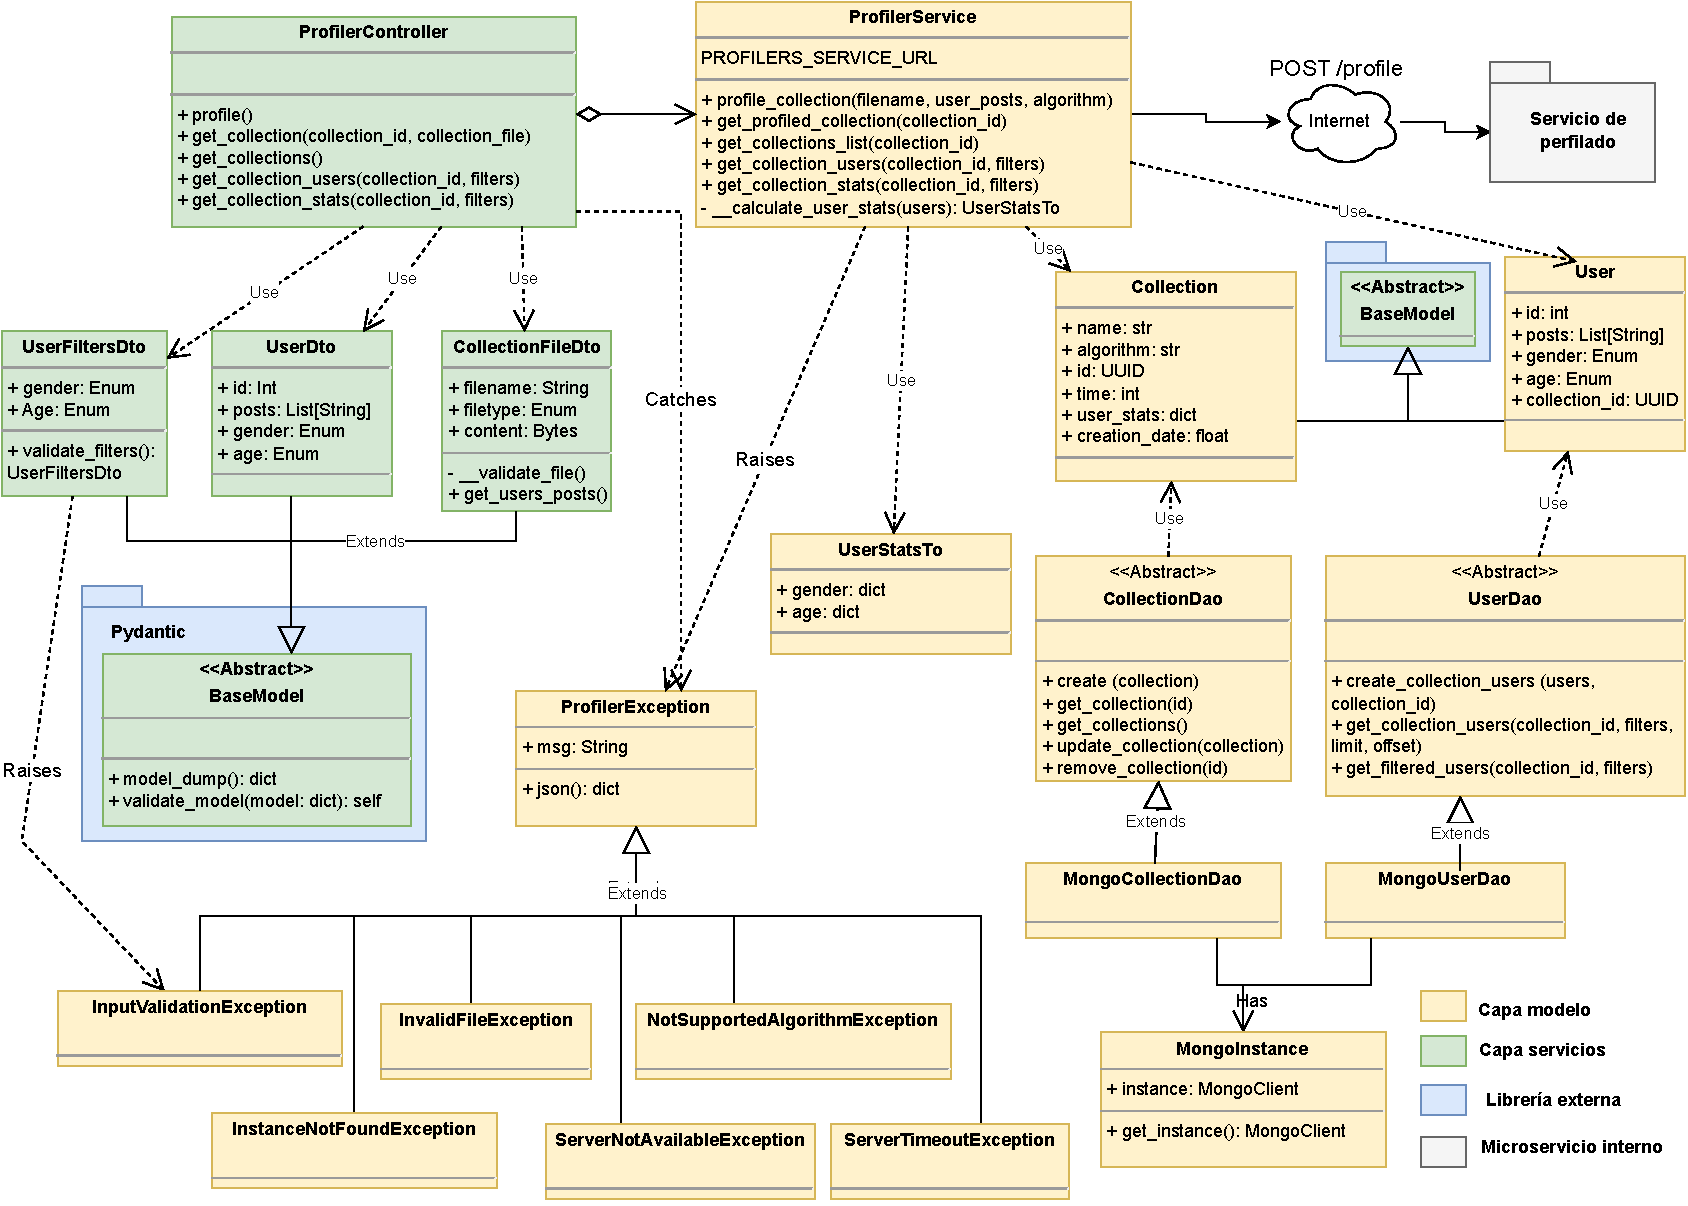
\includegraphics[width=\textwidth]{imaxes/diagramas/backend-classes.pdf}
  \caption{Diagrama de clases final del API REST del sistema.}  \label{fig:diagrama/api}
\end{figure}

\subsection{Micro-servicio de perfilado}
En cuanto al micro-servicio de perfilado, se puede comentar que también se ha seguido un enfoque REST, con un único endpoint de entrada, para la comunicación con el \textit{backend}. En el diagrama de la figura \ref{fig:diagrama/micro-servicio}, se puede ver la estructura de este micro-servicio.

\begin{figure}[H]
  \centering
  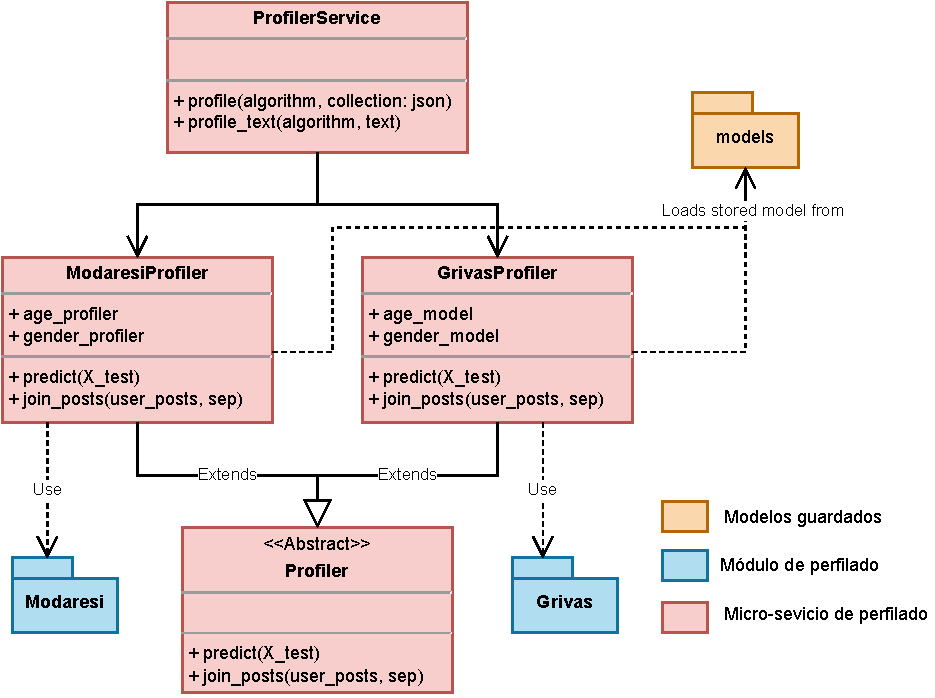
\includegraphics[width=\textwidth]{imaxes/diagramas/profiler-service.pdf}
  \caption{Diagrama de clases final del micro-servicio de perfilado.}  \label{fig:diagrama/micro-servicio}
\end{figure}

En el mismo se muestra que las clases que implementan los \textit{profilers} cargan los modelos y \textit{pipelines} de preprocesado de un módulo llamado <<models>> donde se encuentran todos aquellos modelos necesarios ya entrenados y listos para el perfilado de los algoritmos.

Estos modelos guardados tienen dependencias con los módulos de perfilado, que se ven color azul en el diagrama, que son aquellos que contienen el código para el preprocesado y creación de los modelos de aprendizaje automático. Sin embargo, como son módulos de autores externos adaptados para el proyecto se decidió no mostrar su estructura en el diagrama de clases.

% \subsection{\textit{frontend}}
 \chapter{Desarrollo}
\label{chap:desarrollo}
\lettrine{E}{ste} capítulo contiene la descripción en detalle de las tareas e historias de usuario llevadas a cabo en cada incremento realizado durante el transcurso de este proyecto. Aquí, se les da contexto y se expone el proceso llevado a cabo para su realización, incluyendo decisiones de diseño tomadas durante las mismas.

\section{Sprint 1: Configuración del entorno e investigación del estado del arte}
Este período constituye el primer incremento del proyecto propiamente dicho\footnote{Aunque antes se realizaran ciertas tareas de configuración del entorno y introducción al estado del arte se incluyen en este incremento debido a la poca carga de trabajo de las mismas.}. Junto al segundo \textit{sprint} constituyen los incrementos con menor carga de trabajo del mismo. Las tareas llevadas a cabo durante el este período se pueden dividir en dos conjuntos según la naturaleza más teórica o más práctica de las mismas.

Empezando por las tarea de naturaleza más teórica, está la introducción y familiarización con el estado del arte de la temática a desenvolver. Para ello se optó por el estudio acerca del perfilado automático de usuarios a través de diversos trabajos \citep{profiling_urdu, radivchev2019celebrity, pronouns_paper}. Esta tarea generó la necesidad de comprender las técnicas y conceptos de procesado de lenguaje natural usados en los mismos.

En paralelo, se realizaba la tarea más práctica de configuración del entorno y experimentación con bibliotecas de \acrshort{nlp}. Las dos librerías fundamentales que se utilizaron fueron \textit{Spacy}\footnote{\url{https://spacy.io/}} y \textit{NLTK}\footnote{\url{https://www.nltk.org/}}\footnote{A pesar del uso inicial de estas librerías, a modo de herramientas de estudio, en este incremento; el hecho de que no se utilizaran para el desarrollo de la aplicación final es el motivo por el que se decidió no incluirlas en la sección~\ref{chap:tecnologias} de tecnologías usadas.}.

A la vez que se iban viendo las técnicas usadas en los trabajos estudiados, se aplicaban las mismas para la experimentación en cuanto al preprocesado de los textos de la colección objetivo. De esta forma, se seleccionaba aquellas que se pensaran que iban a ser más efectivas en el contexto de los textos a perfilar: comentarios de redes sociales donde predomina un lenguaje informal, plagado de vulgarismo y emoticonos. Es decir, también se iba realizando una exploración previa acerca de las características de la colección y problemas que pudieran surgir. Con estas circunstancias se dio importancia a técnicas de preprocesado como lematización de las palabras, o sustición de emojis por su significado. 

\section{Sprint 2: Comparación y selección de algoritmos y \textit{datasets}}
En este segundo \textit{sprint}, la primera tarea abordada en el mismo consistió en resolver el problema explicado en la sección \ref{sec:datasets} de la memoria. Este consistía en no poder disponer de un subconjunto de usuarios ya etiquetados a modo de \textit{dataset} de entrenamiento de la colección objetivo liberada por \citet{heritage_BLM}. Como se comenta en el apartado mencionado, la solución al mismo pasó por la selección y obtención de un corpus de entrenamiento externo, disponible; que se realizó en este incremento.

Al margen de eso, la otra tarea fundamental fue la de la búsqueda, investigación y selección de algoritmos de perfilado automático en español del estado del arte, que se explica en detalle en la sección~\ref{sec:estado_arte}. En este momento, la variedad de aproximaciones distintas en algoritmos de perfilado automático basados en texto, sumada a la relativa complejidad de los modelos del estado del arte en este campo hizo que nos centráramos en la tarea de adaptar a nuestro problema alguno de los algoritmos de perfilado con buen rendimiento demostrado, que se encontraran disponibles en forma de código abierto. Pues, el intentar construir diferentes algoritmos de perfilado propios, 
partiendo de cero o aún tratando replicar el trabajo realizado por otro autor, incrementaría el riesgo de desviarnos demasiado del objetivo final del proyecto, debido a la dificultad de la tarea.

Además también en este período también se procedió a realizar la carga del corpus de \acrshort{blm} en forma de fichero en un formato orientado a datos que pudiera ser más manejable desde librerías de \acrshort{aa}. En este paso se incluye la agrupación de usuarios y el filtrado de ruido en el corpus como publicaciones vacías.

\section{Sprint 3: Algoritmo de \citet{loscalis22} y \textit{scraper}}

En este \textit{sprint}, se procedió a realizar la adaptación del \textit{profiler} usado en la primera aproximación del capítulo~\ref{chap:fundamentos} de la memoria. Esta adaptación conforma un primer paso de la historia de usuario \hyperref[tab:user-stories]{E1}, la cual se puede catalogar más bien como una épica que una historia de usuario corriente.

Para la adaptación de este algoritmo a nuestro problema, el primer paso fue tratar de replicar los resultados obtenidos por \citet{loscalis22} en la competición del IberLef 2022 \citep{iberlef2022}, basándonos en el código fuente del mismo\footnote{Disponible en \url{https://github.com/ssantamaria94/PoliticES2022/blob/main/PoliticES.ipynb}.}. Esto fue menos sencillo de lo que pudiera parecer en un comienzo debido a varios factores:

\begin{itemize}
    \item La nula experiencia del estudiante con una librería avanzada de redes neuronales como es Tensorflow.
    \item El gran coste computacional del modelo que acarrea la necesidad del uso de hardware especializado, como es el caso de una \acrshort{tpu} para las pasos de creación, entrenamiento y predicción de nuevas instancias.
    \item El hecho de que las versiones actuales de Tensorflow no son compatibles por algún motivo con la implementación concreta del modelo de \citet{loscalis22}. El problema radicaba en que el código no daba ningún error de usuario, sin embargo, al realizar el entrenamiento el modelo no convergía exitosamente hacia un mínimo local, lo que era bastante confuso para el estudiante pues se sabía que el mismo debía dar buenos resultados. Este error se solucionó usando la versión concreta especificada en las \textit{working notes} de los autores.
\end{itemize}

Al mismo tiempo que se realizaba esta adaptación, se procedió a la creación del \textit{scraper} para la descarga del conjunto de datos explicada en el apartado~\ref{subsec:dataset2016}. Como se comentó en esa sección, la descarga de la totalidad del \textit{dataset}, resultó en un pequeño cuello de botella para el progreso del \textit{sprint}, durando varios días debido a la lentitud de la ejecución del \textit{scraper}.

Una vez realizada la adaptación al problema en cuestión del modelo, se procedió a la toma de resultados y posterior intento de mejora del rendimiento del algoritmo (el cual resultó poco fructífero) que se documentaron en el apartado~\ref{subsec:1aprox}.

\section{Sprint 4: Algoritmos restantes y obtención de resultados}

En este período se priorizó la ejecución de otras dos tareas relacionadas con la épica \hyperref[tab:user-stories]{E1} como: la adaptación de los algoritmos de \citet{grivas2015author, modaresi:2016}. \footnote{Disponibles en \url{https://github.com/pan-webis-de/grivas15} y \url{https://github.com/pan-webis-de/modaresi16} respectivamente.}

La adaptación de estos dos algoritmos fue similar. Ambos están escritos en una versión antigua de Python (anterior a la 3), se cree que la 2.7. El caso es que al ser \gls{legacy-code}, siguiendo la guía de ejecución basada en la creación de un entorno virtual de python, como se indicaba en el repositorio de \citet{grivas2015author} no era posible ejecutar el algoritmo mencionado aún utilizando la versión 2.7 de python, debido a problemas con las dependencias. Por otra parte, el algoritmo de \citet{modaresi:2016} proponía su ejecución a través de un contenedor Docker el cual ya estaba especificado en el repositorio. Sin embargo, en la práctica tampoco era posible ejecutarlo debido a que la imagen base del mismo estaba obsoleta. Por otro lado, también se trató de crear un entorno virtual local para la ejecución de este último, que igualmente resulto inútil.

Ante estos problemas, la alternativa que se presentaba como más prometedora era la de hacer una migración de este código obsoleto hacia unas versiones más recientes del lenguaje y sus dependencias, que contaran soporte actual. Sin embargo, esta alternativa también se descartó principalmente por un motivo: estas implementaciones usaban algunas librerías propias de los autores\footnote{Como es el caso de \url{https://pypi.org/project/tictacs/}} u otras ya obsoletas, las cuales sería necesario reemplazar ya que no están mantenidas actualmente. 

La idea de hacer modificaciones demasiado grandes en estas implementaciones era algo no deseado debido a que podía hacer imposible la replicación de los resultados obtenidos por estos, el cual era un objetivo prioritario. Con lo cual, la otra opción que se probó fue la de tratar modificar el contenedor Docker de \citet{modaresi:2016} para hacerlo funcional. Esto se consiguió tras varios intentos fallidos con distintas imágenes base hasta que una de \textit{Ubuntu:18.04} dio con el cable. Tras conseguir hacerlo operativo para el algoritmo de \citet{modaresi:2016}, se hicieron unas pequeñas modificaciones y también se pudo utilizar para la implementación de \citet{grivas2015author}.

Después de completar estas tareas, se procedió a la ejecución de pruebas con estos modelos que se documentaron en los apartados \ref{subsec:2aprox} y \ref{subsec:3aprox} de la memoria. 

\section{Sprint 5: Desarrollo del micro-servicio de perfilado}
Durante este incremento, se procedió a la redacción de los dos primeros capítulos de esta memoria a partir los resultados obtenidos en los últimos incrementos. Estos correspondían, a la parte con una vertiente más orientada a la investigación del proyecto. A partir, de este momento se comenzó con el desarrollo en sí de la aplicación final.

Para ello, se comenzó con el backend para dar el penúltimo paso para el desarrollo de la épica \hyperref[tab:user-stories]{E1}, antes del desarrollo de la interfaz de usuario. Así se entrenaron los modelos elegidos para producción y se guardaron estos en un fichero binario mediante la librería Joblib\footnote{\url{https://joblib.readthedocs.io/en/stable/}}. Para de esta forma, poder cargar estos modelos más rápidamente, sin necesidad de entrenarlos cada vez al arrancar la aplicación, favoreciendo el rendimiento y escalabilidad (\hyperref[tab:user-stories]{RNF-5}) de la misma. Por otro lado, mediante Flask se creó una API REST muy simple con un único \textit{endpoint} para la operación de perfilado de un \textit{dataset}. Esta aplicación instanciaría los modelos de perfilado al arrancar para luego poder llamarlos ante una petición. Esta pequeña API es la que constituiría el micro-servicio de perfilado de la aplicación (ver \ref{sec:arquitectura}).

Sin embargo, en este punto se identificó un problema no previsto relacionado con el \textit{profiler} adaptado de \citet{loscalis22}. El hecho de almacenar los modelos ya creados y entrenados nos aliviaba esa carga computacional que en el caso de este modelo concreto era inasumible sin la utilización de hardware especializado del que no contábamos. No obstante, lo que no estaba previsto era que el empleo de este modelo simplemente para el procesado y predicción de una colección de usuarios era igualmente inasumible, debido a que se iba el tiempo de perfilado de una colección del tamaño de \acrshort{blm} a más de una hora. Por este motivo, se decidió prescindir de este algoritmo para la aplicación final, al no contar con hardware especializado para su ejecución.

Finalmente, otra tarea que se realizó fue el diseño de la interfaz de usuario para el cliente web de la aplicación, mediante la realización del prototipado de la misma (sección \ref{sec:prototipo}).

\section{Sprint 6: Inicio del \textit{frontend} y primeras visualizaciones}
Aquí se comenzó con el desarrollo del \textit{frontend}. En este punto ya se había tomado la decisión de tener una separación entre capas, con la separación de \textit{backend} y \textit{frontend}. Sin embargo, aún quedaba la decisión si crear una SPA o usar SSR con un framework como Next.js\footnote{\url{https://nextjs.org/}} para React. En nuestro caso, se optó por la primera alternativa a pesar de las desventajas asociadas a las mismas como problemas de \gls{seo} o peor rendimiento en el navegador, debido principalmente a la poca experiencia del estudiante con estas librerías. Además se completaron las siguientes historias de usuario:
\begin{itemize}
    \item \hyperref[tab:user-stories]{E1 y H2}: al añadir el cliente web, finalmente se dio por finalizada la épica de \textbf{perfilar un \textit{dataset}} y además se completó igualmente la historia de poder \textbf{elegir el algoritmo de perfilado}. Para ello, se creó un formulario con dos campos el fichero que corresponde a la colección que se quiere perfilar, de carácter obligatorio; y un desplegable para el algoritmo a utilizar. Además se añadieron comprobaciones tanto en la parte cliente, como en el \textit{backend} para que el fichero tuviera el tipo adecuado y las columnas necesarias. Por otro lado, se creó un \textit{spinner} a modo de feedback mientras se estuviera perfilando el \textit{dataset}.
    \item \hyperref[tab:user-stories]{H4 y H7}: se crearon unas visualizaciones en forma de \textbf{gráfico} para poder ver la distribución de usuarios por \textbf{edad} y \textbf{género}. Se optó por un gráfico de barras para la edad, debido principalmente a dos motivos: estos son más adecuados para comparar variables donde existen más de dos categorías, que por ejemplo un gráfico en forma de tarta donde puede no ser tan inmediato saber cual porción es mayor. La otra razón, es que las categorías tienen un orden, es decir, el grupo de 18-24 es más joven que el de 25-34, este a su vez que el de 34-49, etc.
    
    Por otro lado, al contrario que la edad el género no es una variable que tenga un orden en el mundo real, esto sumado al hecho de que solo se quieran comparar dos categorías hace que un gráfico en forma de tarta se considerase la mejor opción, debido a su simplicidad y estética. Además, estos resaltan de mejor forma que los gráficos de barras porcentajes o partes de un todo, como puede ser la porcentaje de usuarios de un género sobre el total. En este sentido, se consideró adecuado este gráfico también para representar la edad, no obstante, se prefirió usar únicamente un gráfico por atributo.
\end{itemize}

En este punto se estaba persistiendo la colección perfilada dentro de cada sesión del navegador, a través del almacenamiento web. Sin embargo, este almacenamiento tiene limitaciones en cuanto al tiempo y espacio disponible. Por este motivo, surge la necesidad de usar una base de datos para almacenar las colecciones perfiladas. Al mismo tiempo, nos damos cuenta que solo la visualización de los gráficos no nos aporta información sobre el tipo de publicaciones que realizaba un usuario según el género o edad que le fuera asignado.

Para responder a estas necesidades se programó para el siguiente \textit{sprint} la tarea de añadir persistencia a la aplicación mediante una base de datos, así como las historias de usuario \hyperref[tab:user-stories]{H3} y \hyperref[tab:user-stories]{H6}.

\section{Sprint 7: Lista y detalle de usuarios}

Como se adelantó en la sección anterior, en este \textit{sprint} se añadió persistencia a través de una base de datos. Para ello, lo primero fue crear un módulo separado del micro-servicio de perfilado que sirviera como medio para la comunicación del \textit{frontend} con la base de datos y el micro-servicio de perfilado. Esta acción tenía dos objetivos principales: mantener la separación de responsabilidades entre capas y no extender el código del micro-servicio de perfilado que mantiene una versión de Python obsoleta (2.7), para de esta manera favorecer la extensibilidad y mantenibilidad el código (\hyperref[tab:rnf]{RNF-2}). 

Este conformaría el \textit{backend} (que cumple la función de API REST) en la arquitectura final (\ref{sec:arquitectura}). Así, cada vez que se recibiera una llamada para perfilar una colección del \textit{frontend}, el \textit{backend} se encargaría de delegar esta responsabilidad en el micro-servicio y posteriormente devolvería la colección perfilada por este último, a la vez que la almacenaría en base de datos.

Como base de datos, se optó por una no relacional como ya se comentó en el capítulo~\ref{chap:tecnologias}. Principalmente, debido a la posibilidad de escalarla horizontalmente de manera sencilla, así como a la flexibilidad que ofrece MongoDB, ya que al ser una base de datos basada en documentos no está atada a un esquema de datos concreto. Otra motivo importante, es la naturaleza no transaccional de los datos almacenados.

A continuación, se aprovechó para encapsular cada módulo en un contenedor Docker, uno para cada elemento de la arquitectura (véase figura \ref{fig:diagrama/arquitectura}), y crear un archivo \textit{docker-compose.yml}. Con este, se pretende facilitar el arranque simultáneo de distintos módulos, a la vez que se realiza la configuración las dependencias entre ellos y la red para la inter-comunicación sin necesidad de exponer puertos innecesariamente al exterior. De esta manera, se favorecen la seguridad, mantenibilidad y portabilidad del sistema (\hyperref[tab:rnf]{RNF-2} y \hyperref[tab:rnf]{RNF-4}).

A continuación, se implementaron las historias de usuario \hyperref[tab:user-stories]{H3} y \hyperref[tab:user-stories]{H6} para poder \textbf{ver la lista de usuarios} y \textbf{ver las publicaciones de un usuario} en detalle, respectivamente. Para ello, en el API se creó una operación GET para poder recuperar los usuarios de una colección perfilada de forma paginada. Así, en el \textit{frontend} se creó la capa de acceso a servicios para las llamadas al API, un componente para mostrar la lista de usuarios y una página distinta para ver el detalle de un usuario. Asimismo se aprovechó para mejorar la estética de la interfaz web en general y se incorporó la utilización \textit{CSS Modules} \footnote{\url{https://github.com/css-modules/css-modules}} para una mejor organización de los estilos.

\section{Sprint 8: Persistencia y rediseño del \textit{Dashboard}}
Aunque en el anterior incremento se añadió la funcionalidad mencionada relacionada con la persistencia del \textit{backend}, entonces, no se le dio importancia al seguimiento de unas buenas prácticas de diseño, al no realizar una correcta separación entre capa servicios, capa modelo y acceso a datos. Por este motivo, en este \textit{sprint} donde se tenía programado implementar la historia de usuario \hyperref[tab:user-stories]{H5} que involucraba añadir detalles generales de la colección a la base de datos, se vió necesario realizar una buena refactorización de la gestión de la persistencia, el enrutado en el \textit{frontend}, y sobre todo el modelo de datos y gran parte del \textit{backend}.

De esta manera, se comenzó por el servidor. En la API, se reorganizó el código de forma que hubiera una separación lógica entre controlador y modelo. También se modeló la conexión a la base de datos como un \textit{singleton} y se añadieron abstracciones de clases \acrshort{dao} para modelar el acceso a la base de datos mediante operaciones \acrshort{crud}, desacoplando de esta manera el API de la base de datos concreta que se emplee. Del mismo modo, se añadieron validaciones en la capa servicios o controlador mediante la creación de \acrshort{dto}s, con la librería \textit{Pydantic} ya mencionada en~\ref{chap:tecnologias}.

A pesar de estar usando una base de datos no relacional, orientada a documentos, como MongoDB, la cual no necesita emplear <<colecciones>> distintas (corresponden a las tablas SQL, en terminología de MongoDB) para modelar una relación entre dos entidades, debido a que se puede hacer uso de <<documentos>> o <<colecciones>> anidadas, se juzgó apropiado separar las entidades (modeladas en el \hyperref[fig:diagrama/ER]{diagrama entidad-relación}) en dos colecciones Mongo distintas. Esto se justifica por los siguientes motivos: 

\begin{itemize}
    \item Por un lado, ambas colecciones tienen patrones de lectura y acceso distintos: mientras que la entidad \textit{Colección} se espera que se acceda una vez al cargar el \textit{Dashboard} de una colección, la entidad \textit{Usuarios} se accede cada vez que se hace \textit{scroll} en la lista paginada de los mismos. El usar dos colecciones distintas permite almacenar las entidades de forma separada optimizando los accesos a cada una lo que favorece el rendimiento y escalabilidad (\hyperref[tab:rnf]{RNF-5}).
    
    \item Además, el uso de dos colecciones separadas se alinea con la idea de usar dos objetos \acrshort{dao} distintos para cada una. Esto beneficia la mantenibilidad al permitir en un futuro el cambio hacia otro tipo de base de datos como por ejemplo una relacional, donde esta separación lógica se vuelve necesaria, sin apenas modificaciones de la capa de acceso a datos.
\end{itemize}

Tras estas modificaciones en el servidor, se continuó por actualizar la capa acceso a servicios del \textit{frontend} para reflejar los cambios en el API. Por otro lado, se aprovechó para completar la historia \hyperref[tab:user-stories]{H5} para incluir \textbf{información general de la colección} en el \textit{dashboard}, mejorando de esta manera la utilidad y aspecto del mismo. Al mismo tiempo, se aprovechó para incluir también en el \textit{dashboard}, la lista de usuarios (ya que en el diseño inicial se encontraba a parte) y poder acceder a este sin necesidad de haber perfilado una colección en ese momento, empleando un identificador de una colección perfilada previamente. Así, se completaba la historia \hyperref[tab:user-stories]{H8} para \textbf{acceder a una colección perfilada anteriormente}. 

\section{Sprint 9: Lista de colecciones y filtrado de usuarios}

En este \textit{sprint} se completaron las funcionalidades restantes:
\begin{itemize}
    \item Primero, se completó la relativamente sencilla historia \hyperref[tab:user-stories]{H9} para \textbf{ver un registro de las colecciones perfiladas anteriormente} ordenadas temporalmente de más a menos actuales.
    \item Luego, se finalizó el filtrado de usuarios en base a género y edad (\hyperref[tab:user-stories]{H8}).%Esta historia tuvo mayor carga de trabajo que la anterior sobre todo en el \textit{frontend} para el estilado 
\end{itemize}

Finalmente, se adaptó la interfaz de usuario para que fuera compatible con diferentes dispositivos independientemente del tamaño de la pantalla de estos, es decir, que fuera \textit{responsive}. Favoreciendo así, la usabilidad y portabilidad de la misma (\hyperref[tab:rnf]{RNF-1} y \hyperref[tab:rnf]{RNF-4}).

Además también se aprovechó para arreglar pequeños detalles de la interfaz de la aplicación y temas de accesibilidad, como añadir roles a ciertos elementos HTML (\hyperref[tab:rnf]{RNF-1}).
%\section{Sprint 10: Redacción de la memoria}
%Sprint final del proyecto, en el que se aprovechó para redactar el resto de la memoria del mismo junto con arreglar pequeños detalles de la interfaz de la aplicación y temas de accesibilidad, como añadir roles a ciertos elementos HTML (\hyperref[tab:rnf]{RNF-1})
 \chapter{Análisis colección \#BLM}
\label{chap:blm}

\lettrine{E}{s} importante no olvidar el objetivo inicial de todo el trabajo previo de los anteriores capítulos. Aunque el desarrollo de la herramienta de perfilado es un fin en sí mismo, y se puede aplicar a más casos de uso que el tratamos nosotros, nuestra verdadera motivación consiste en aplicar esta herramienta de perfilado automático de usuarios para obtener información y poder razonar sobre el movimiento social \acrshort{blm}.

Concretamente, en este capítulo se aplicará nuestro sistema para conocer mejor el tipo de usuarios que publicaban en el corpus, en idioma español, construido por \citet{heritage_BLM} en 2020 a modo de archivo social sobre sobre las discusiones acerca de los conflictos raciales motivados por el asesinato de George Floyd. Este corpus se encuentra disponible en \url{https://www.dc.fi.udc.es/~david/hdh2021/}.

\subsection{Procesado corpus}

Al descargar el corpus de la dirección anterior, este viene distribuido entre múltiples archivos XML por cada \textit{thread} o <<hilo>> del subreddit de BLM. Esta agrupación tiene sentido ya que cada <<hilo>> representa un tópico distinto y los comentarios en cada uno tienen un contexto común. Sin embargo, para nuestra finalidad de perfilar cada usuario de la colección tiene mayor importancia usar el mayor número de publicaciones por usuario para que de esta forma las predicciones tengan mayor fiabilidad.
% \begin{verbatim}
% <thread>
%     <id>477</id>
%     <relevant-posts>
%         <id>479</id>
%     </relevant-posts>
%     <posts>
%         <post>
%             <id>479</id>
%             <author>478</author>
%             <body>
%                 >Eso no se de donde lo sacás. Si quieren prohibir el racismo ...
%             </body>
%         </post>
%         ...
%     </posts>
% </thread>

% \end{verbatim}

En este sentido, se procedió a crear un único archivo CSV, con dos columnas: identificador del usuario y texto de la publicación. Este CSV contendrá todas las publicaciones de cada autor de la colección sin tener en cuenta el hilo concreto de cada una. Es importante señalar que no se agrupan las publicaciones de cada autor en una fila, sino que cada publicación de partida se escribe en una fila distinta del CSV. De esta forma, al tener las publicaciones de cada autor separadas, cada algoritmo de perfilado se encarga de unirlas y preprocesarlas de la manera oportuna.

\section{Aplicación}
Posteriormente, tras haber creado este archivo CSV con el conjunto de todas las publicaciones de los autores de \acrshort{blm} ya se puede subir a la aplicación para perfilar el corpus. Para ello, arrancamos la aplicación en el entorno local y accedemos desde un navegador a la dirección de \textit{localhost} en el puerto 3000. Tras este paso se podrá ver una página de inicio como la de la figura \ref{fig:app/home}. En cada figura de esta sección se mostrarán dos subfiguras con las vistas de la aplicación desde: ordenador de sobremesa (\textit{desktop}) y móvil (\textit{mobile}).

\begin{figure}[H]
  \centering
  \begin{subfigure}{0.7\textwidth}
       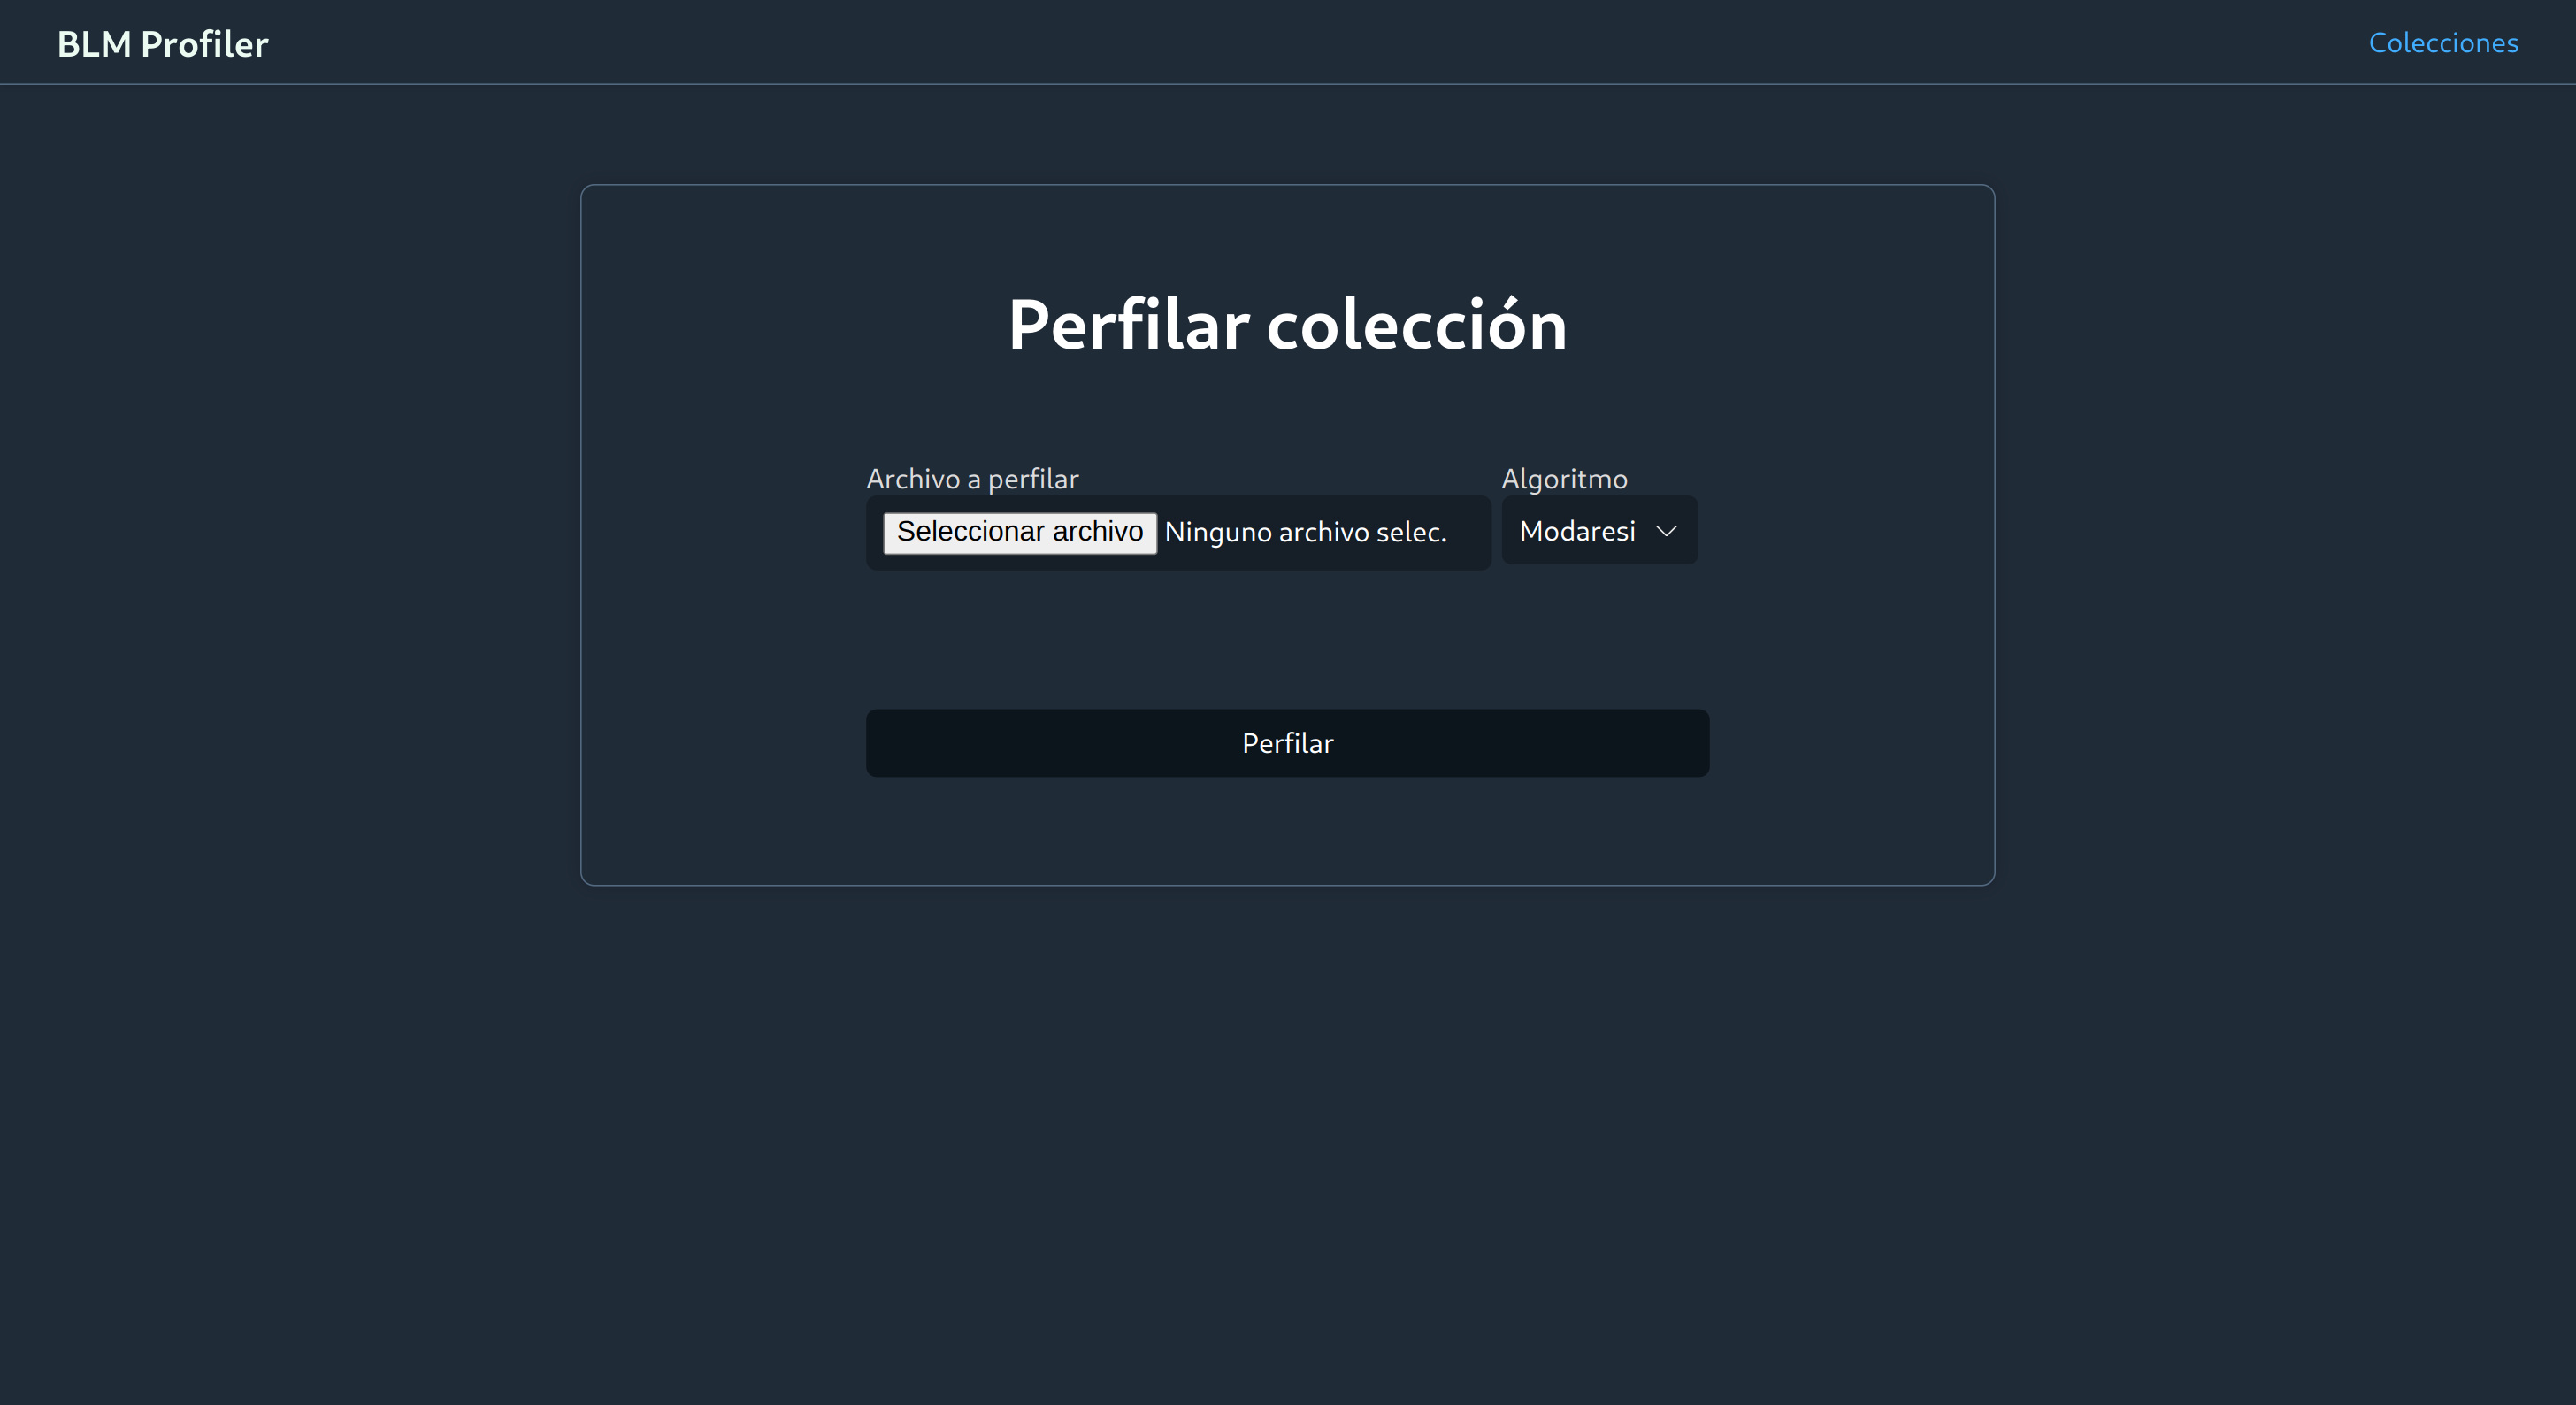
\includegraphics[width=\textwidth]{imaxes/capturas-app/desktop/home.png}
      \caption{\textit{Desktop}} 
  \end{subfigure}
  \begin{subfigure}{0.2215\textwidth}
       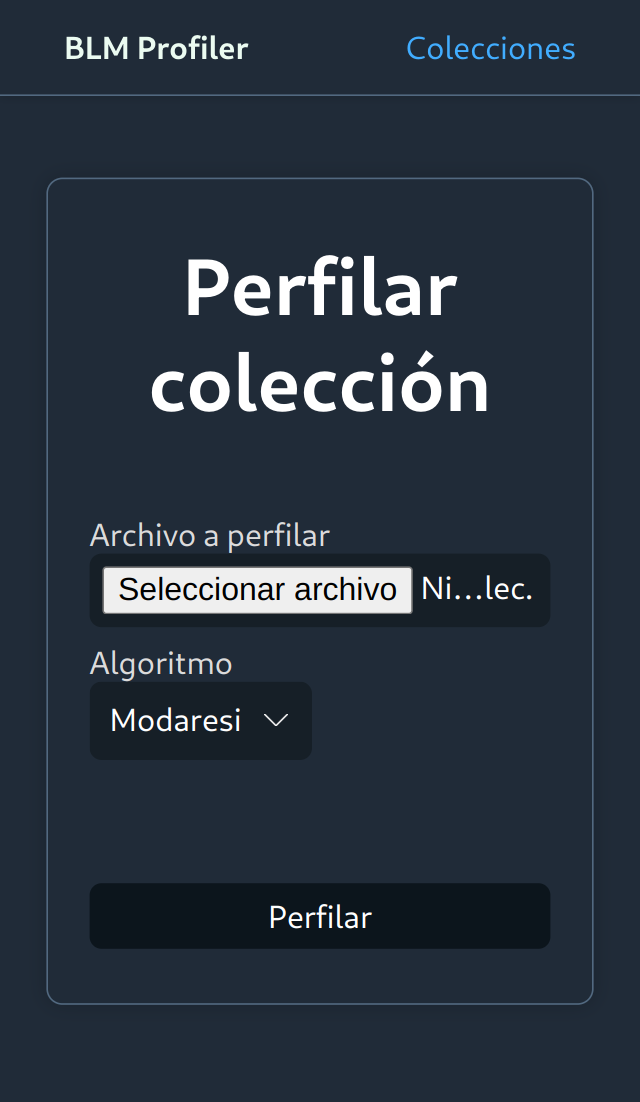
\includegraphics[width=\textwidth]{imaxes/capturas-app/mobile/home.png}
      \caption{\textit{Mobile}} 
  \end{subfigure}
  \caption{Página de inicio.}
  \label{fig:app/home}
\end{figure}
\subsection{Perfilado del corpus}

En esta página se puede ver un formulario con dos campos: uno obligatorio que es el selector del fichero que contiene el corpus a perfilar y otro opcional selector para escoger el algoritmo de perfilado deseado, que por defecto será el de <<modaresi>>. Tras seleccionar el fichero que contiene el corpus a perfilar, que debe tener extensión .csv o .txt, se nos mostrará un mensaje en función de si este es válido o no para el perfilado\footnote{Para que el fichero sea válido debe tener al menos dos columnas llamadas \textit{id} y \textit{posts}, que se refieren al identificador del usuario y su publicación.}. En función de ello nos dejará o no perfilar la colección. Tras este paso, podremos hacer click en el botón de perfilar y la página mostrará un \textit{spinner} a modo de carga mientras se perfila la colección, como se puede ver en la figura \ref{fig:app/home-perfilando}.

\begin{figure}[H]
  \centering
  \begin{subfigure}{0.7\textwidth}
       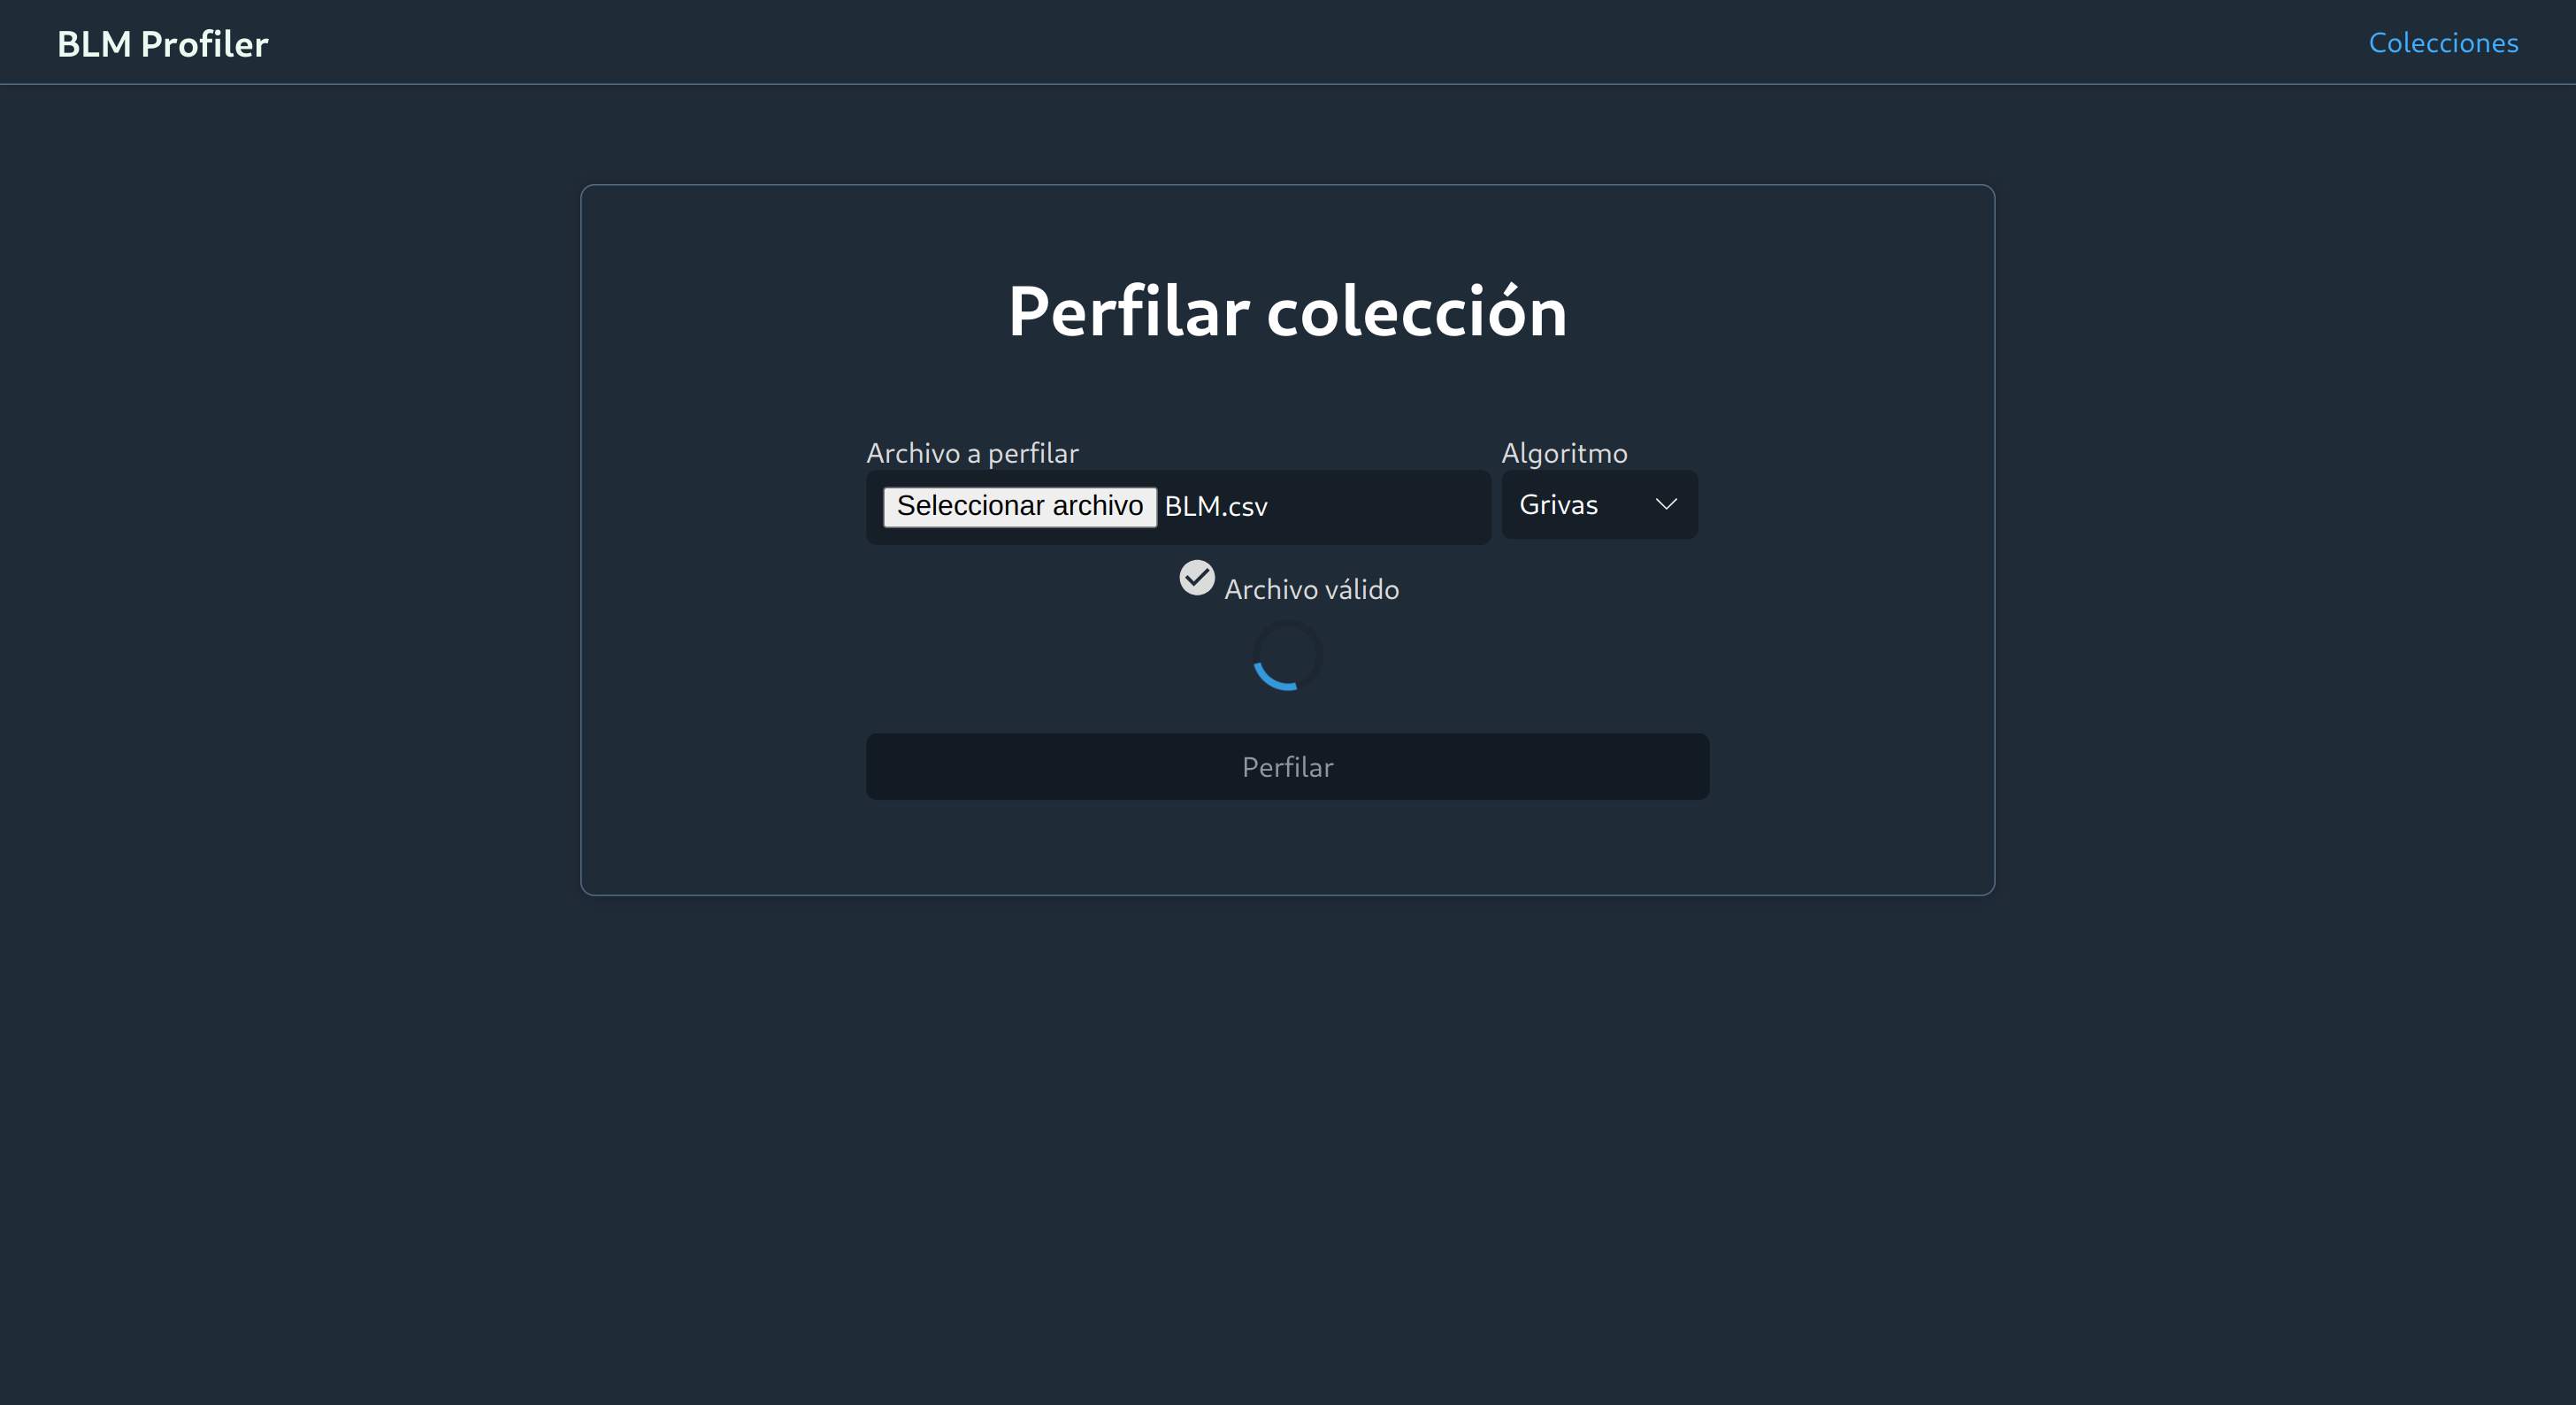
\includegraphics[width=\textwidth]{imaxes/capturas-app/desktop/home_perfilando.png}
      \caption{Desktop} 
  \end{subfigure}
  \begin{subfigure}{0.2215\textwidth}
       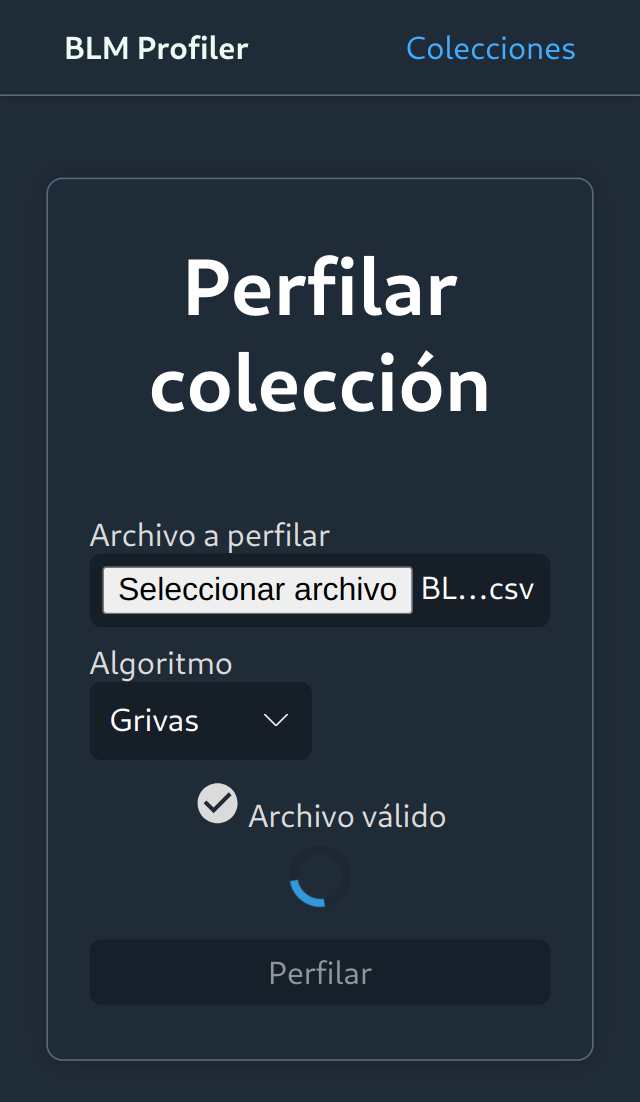
\includegraphics[width=\textwidth]{imaxes/capturas-app/mobile/home_perfilando.png}
      \caption{Mobile} 
  \end{subfigure}
  \caption{Página de inicio mientras se perfila una colección.}
  \label{fig:app/home-perfilando}
\end{figure}
\subsection{Visualización de resultados}

Cuando termine el perfilado la aplicación nos redirigirá al \textit{dashboard} o cuadro de mando de la misma que se puede ver en la figura \ref{fig:app/dashboard}.

\begin{figure}[H]
  \centering
  \begin{subfigure}{0.7\textwidth}
   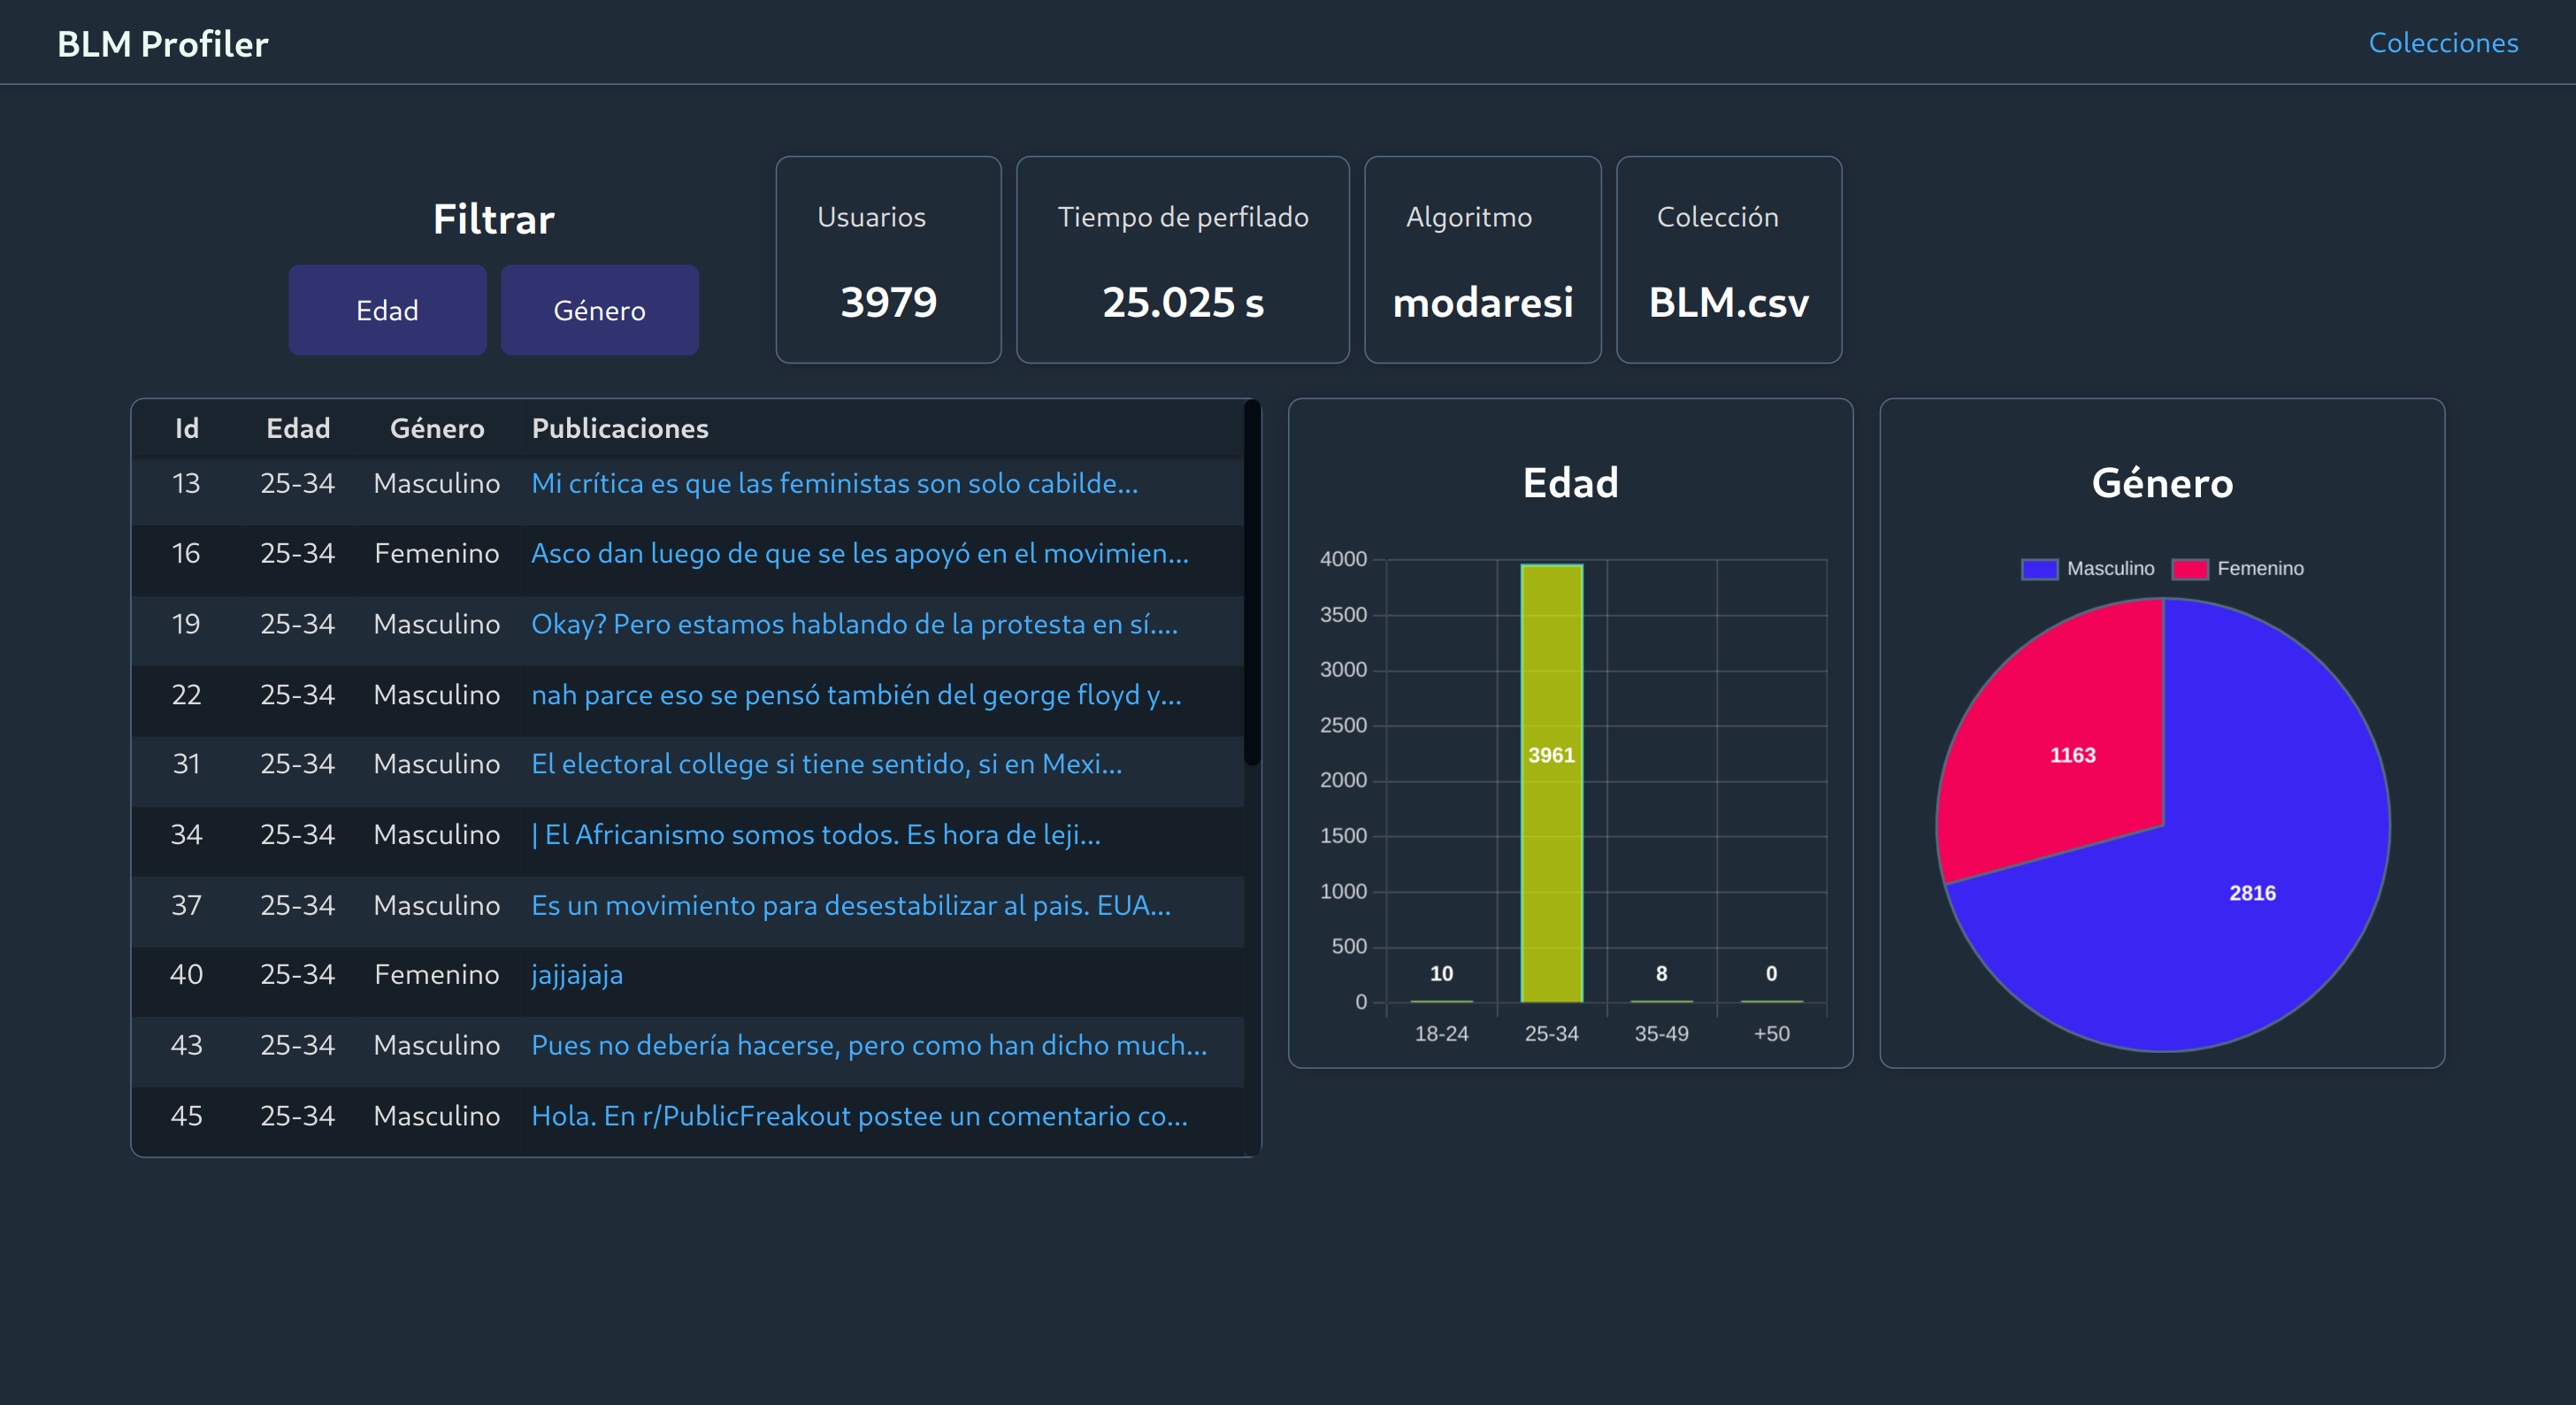
\includegraphics[width=\textwidth]{imaxes/capturas-app/desktop/dashboard.png}
  \caption{\textit{Desktop}} 
  \end{subfigure}
  \begin{subfigure}{0.2215\textwidth}
   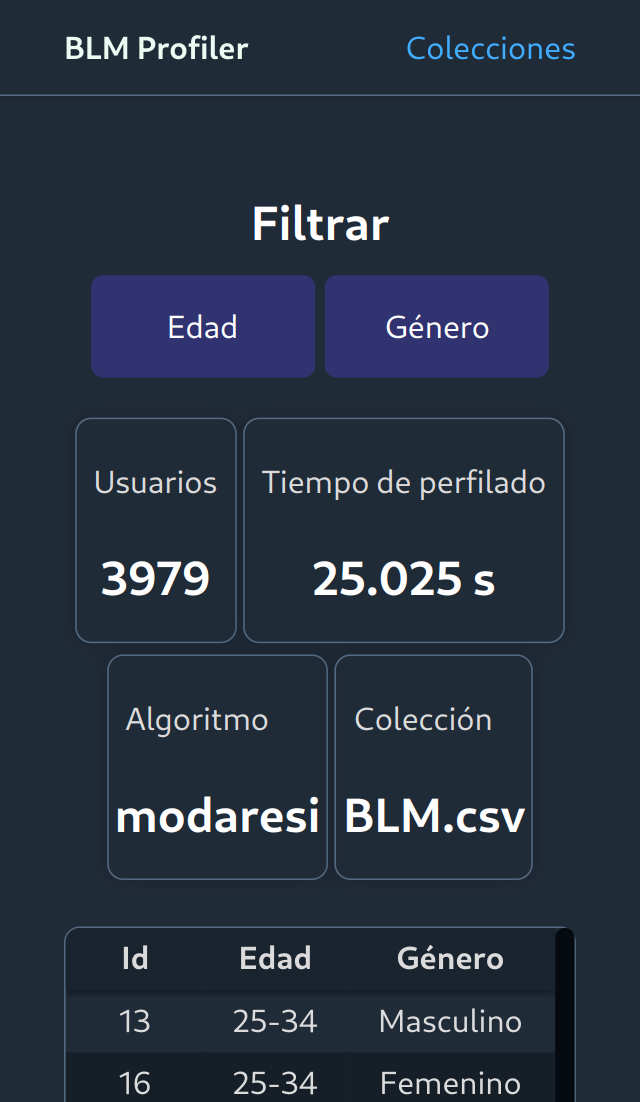
\includegraphics[width=\textwidth]{imaxes/capturas-app/mobile/dashboard.png}
  \caption{\textit{Mobile}} 
  \end{subfigure}
  \caption{\textit{Dashboard} de la colección perfilada.}
  \label{fig:app/dashboard}
\end{figure}

Como podemos ver en la parte de abajo tenemos una tabla y dos gráficos. En el gráfico de barras se puede ver la distribución de los usuarios del corpus según su edad, hay cuatro barras para cuatro rangos de edad distintos. En el gráfico en forma de tarta, en cambio, se muestra la distribución de los usuarios en función del género de los mismos. La tabla, por otra parte, es un listado de todos los usuarios del corpus en el que se muestra el id del mismo\footnote{Correspondiente a la columna id del archivo de subida de la colección}, el género y edad con los que fue clasificado y una muestra de una publicación del usuario en forma de enlace, que explicaremos más adelante.

Luego, en la parte superior, se encuentran varias tarjetas que presentan detalles generales sobre la colección, tales como el tiempo de perfilado, el algoritmo utilizado, el nombre del archivo de subida y el número total de usuarios.

\subsubsection{Filtrado de usuarios por categorías}
Por último, al inicio de la página se encuentra un texto titulado <<Filtrar>> y debajo podemos ver dos botones. Al situar el ratón sobre cualquiera de ellos veremos como realmente son botones desplegables en los que se presentan los posibles filtros para cada categoría. Al seleccionar un filtro de alguna de las categorías veremos como se añade un elemento después de las tarjetas de la colección, que indica el filtro concreto escogido para esa categoría. En la figura \ref{fig:app/dashboard-filtered}, podemos ver el aspecto del filtro añadido.

\begin{figure}[H]
  \centering
  \begin{subfigure}{0.7\textwidth}
   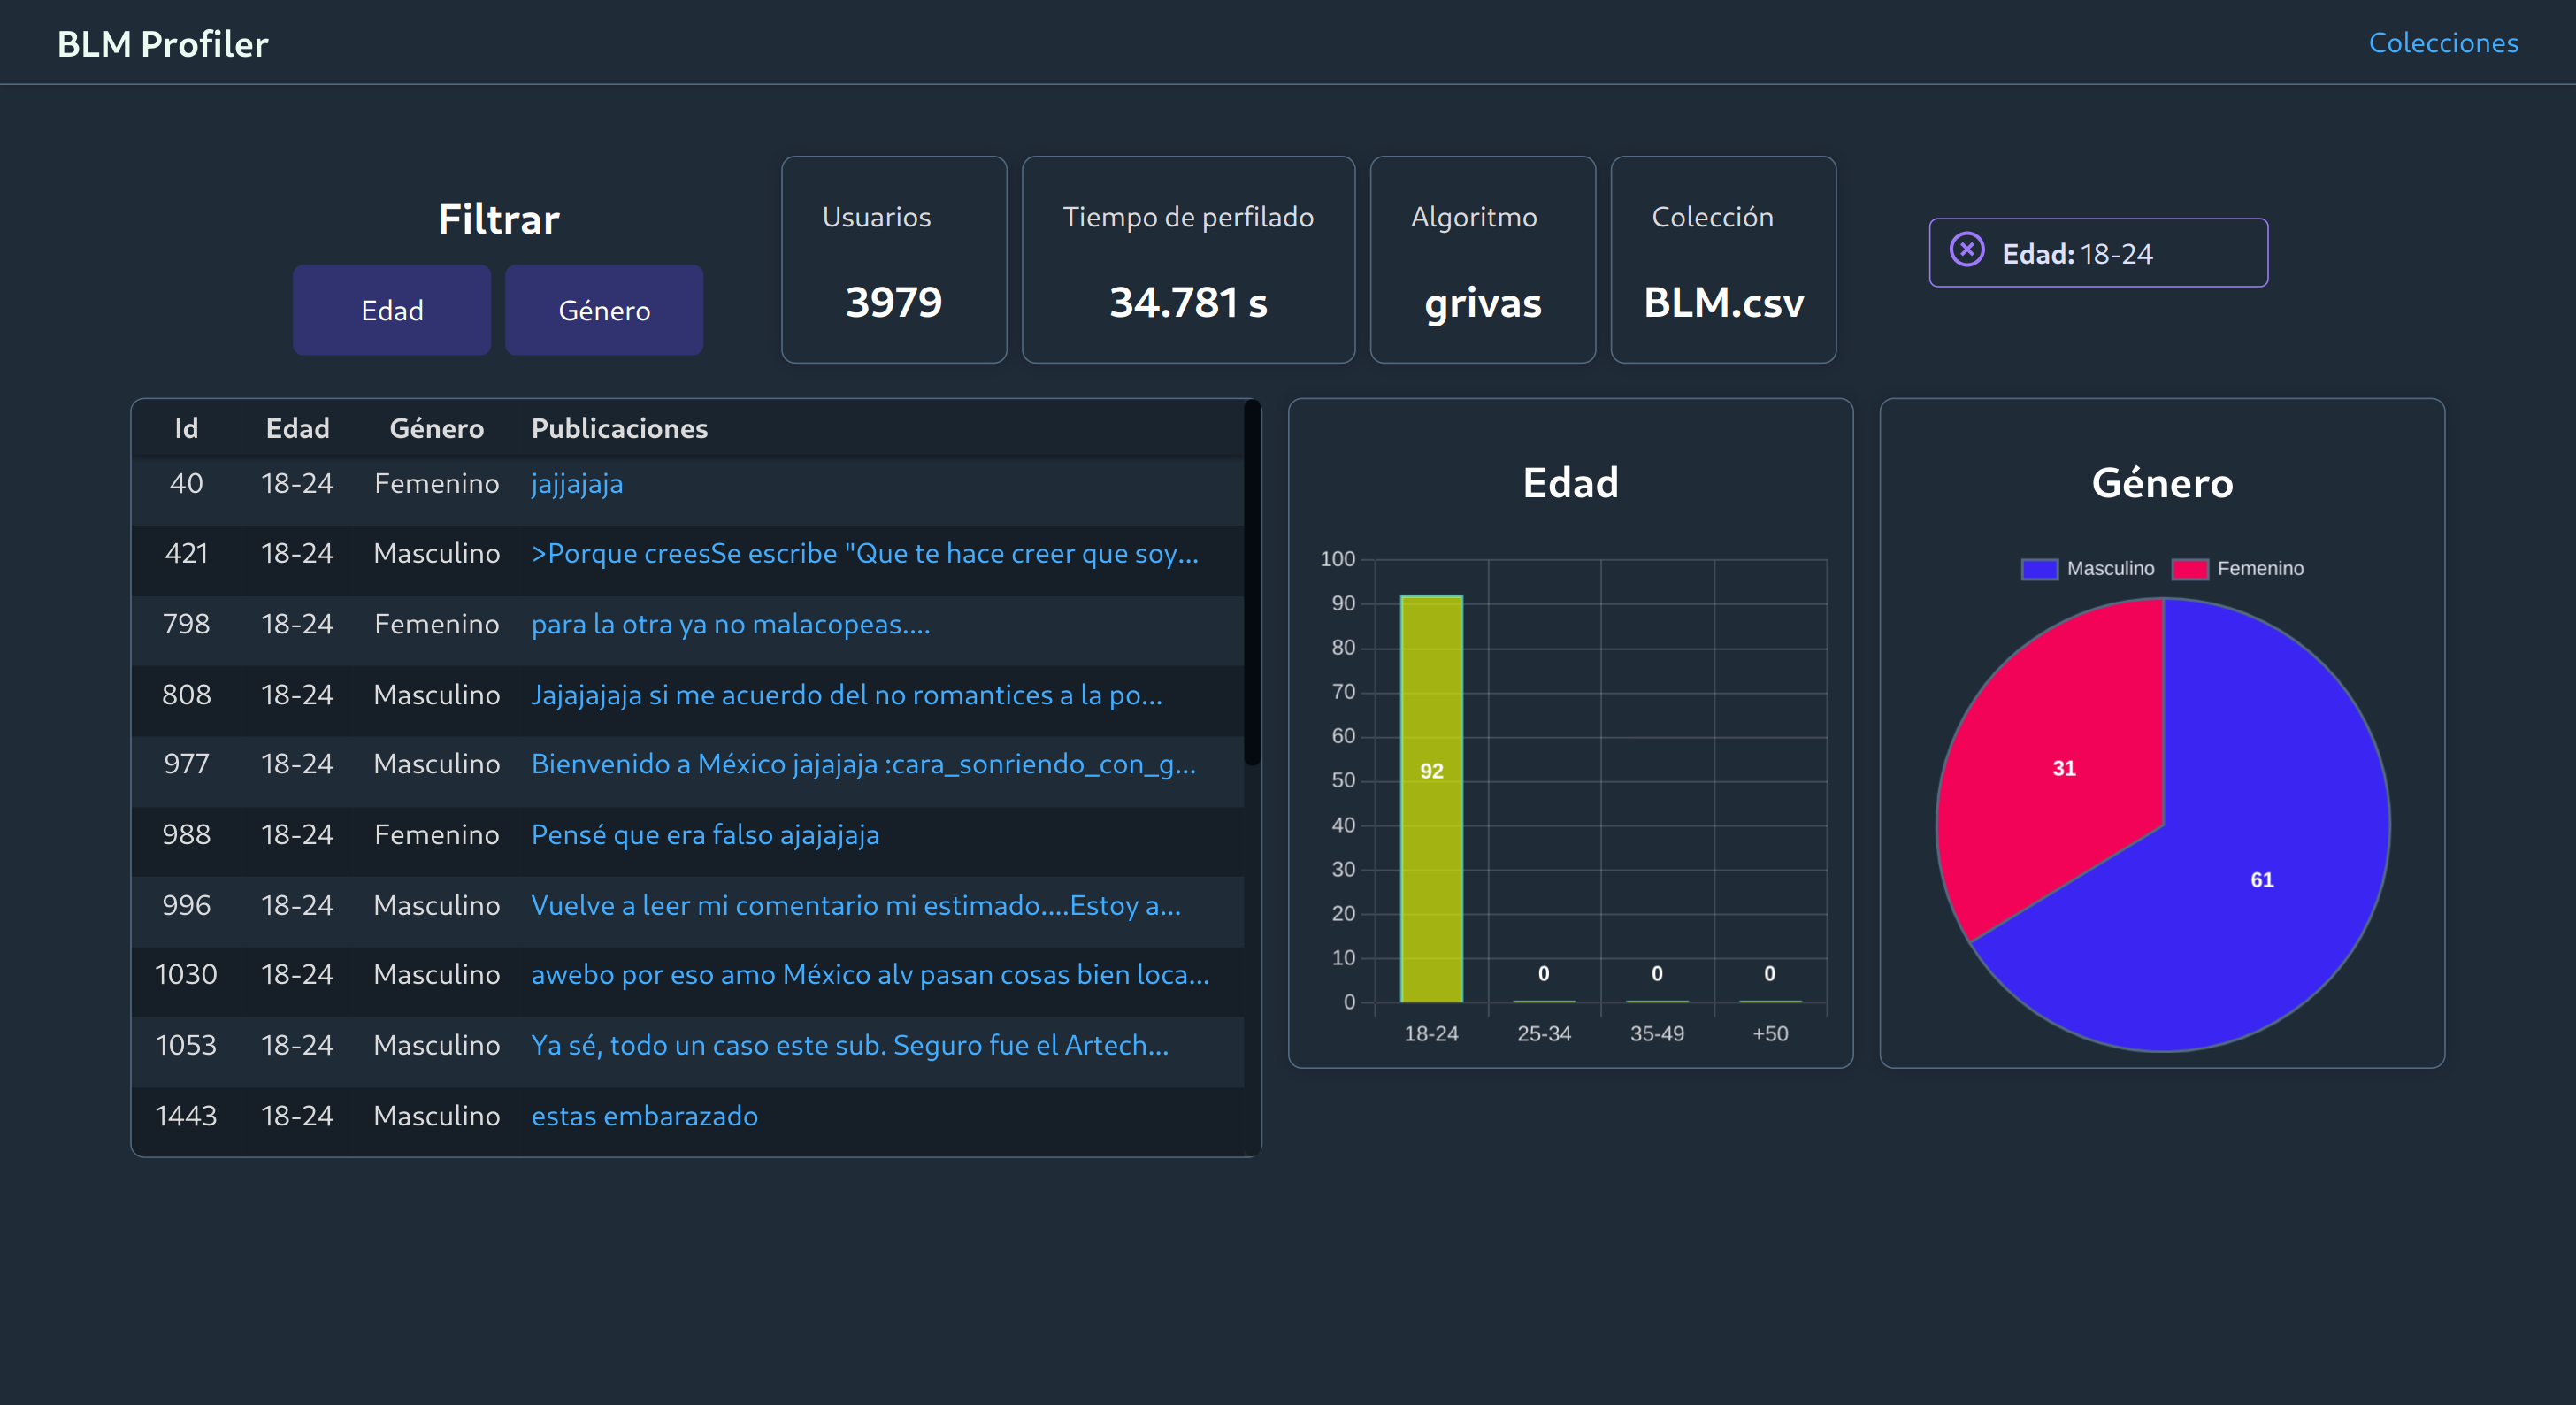
\includegraphics[width=\textwidth]{imaxes/capturas-app/desktop/dashboard-perfilado-edad.png}
  \caption{\textit{Desktop}} 
  \end{subfigure}
  \begin{subfigure}{0.223\textwidth}
   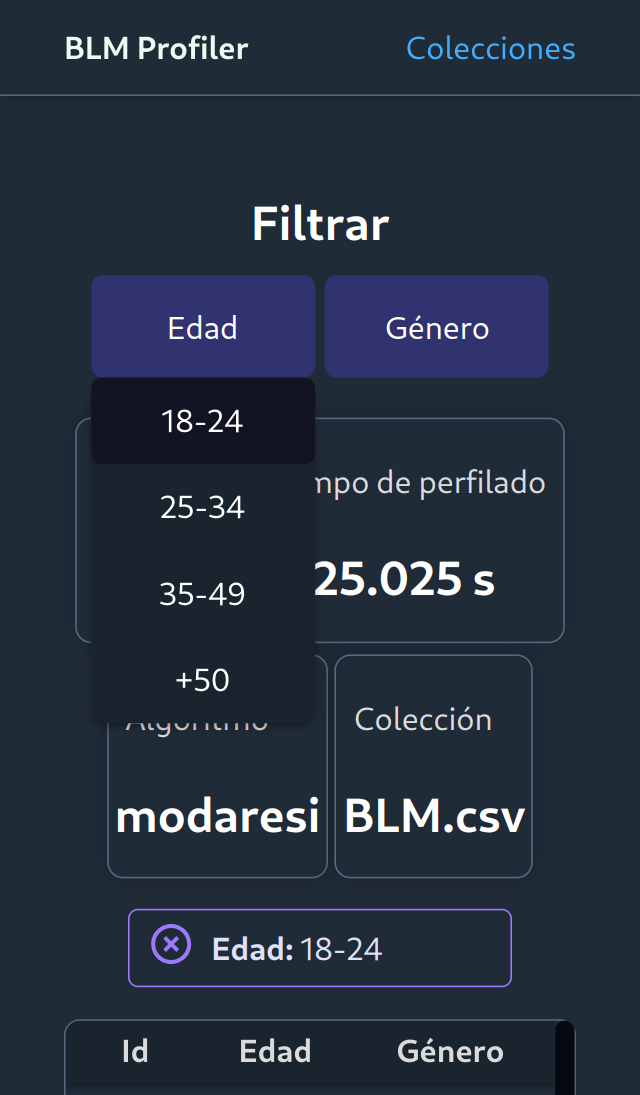
\includegraphics[width=\textwidth]{imaxes/capturas-app/mobile/dashboard-filtrado-edad.png}
  \caption{\textit{Mobile}} 
  \end{subfigure}
  \caption{\textit{Dashboard} de la colección perfilada filtrado únicamente por edad.}
  \label{fig:app/dashboard-filtered}
\end{figure}

Como se puede apreciar en este caso, el proceso de filtrado afecta a la lista de usuarios y a ambos gráficos. Por un lado, en la lista, podemos observar que únicamente se muestran usuarios cuyas edades se sitúan en el rango de 18-24 años. En el gráfico de edad, el filtrado por una grupo de la misma categoría no es especialmente interesante, ya que no nos aporta información nueva. Sin embargo, en el gráfico de género el filtrado por edad nos permite estudiar como cambia la distribución del género de los usuarios en función del rango de edad de los mismos.

Otra opción relevante, es la de filtrar el \textit{dashboard} por ambas categorías. Como ya hemos comentado en los gráficos nos brindaría ninguna información nueva. Por el contrario, al realizar este filtrado podemos estudiar el tipo de publicaciones que realiza un grupo demográfico concreto lo que también nos aporta pistas sobre los criterios que se emplean en el perfilado de cada grupo. En la figura \ref{fig:app/dashboard-filtered-edad-genero}, se puede contemplar el filtrado en función de ambas categorías.

\begin{figure}[H]
  \centering
  \begin{subfigure}{0.7\textwidth}
   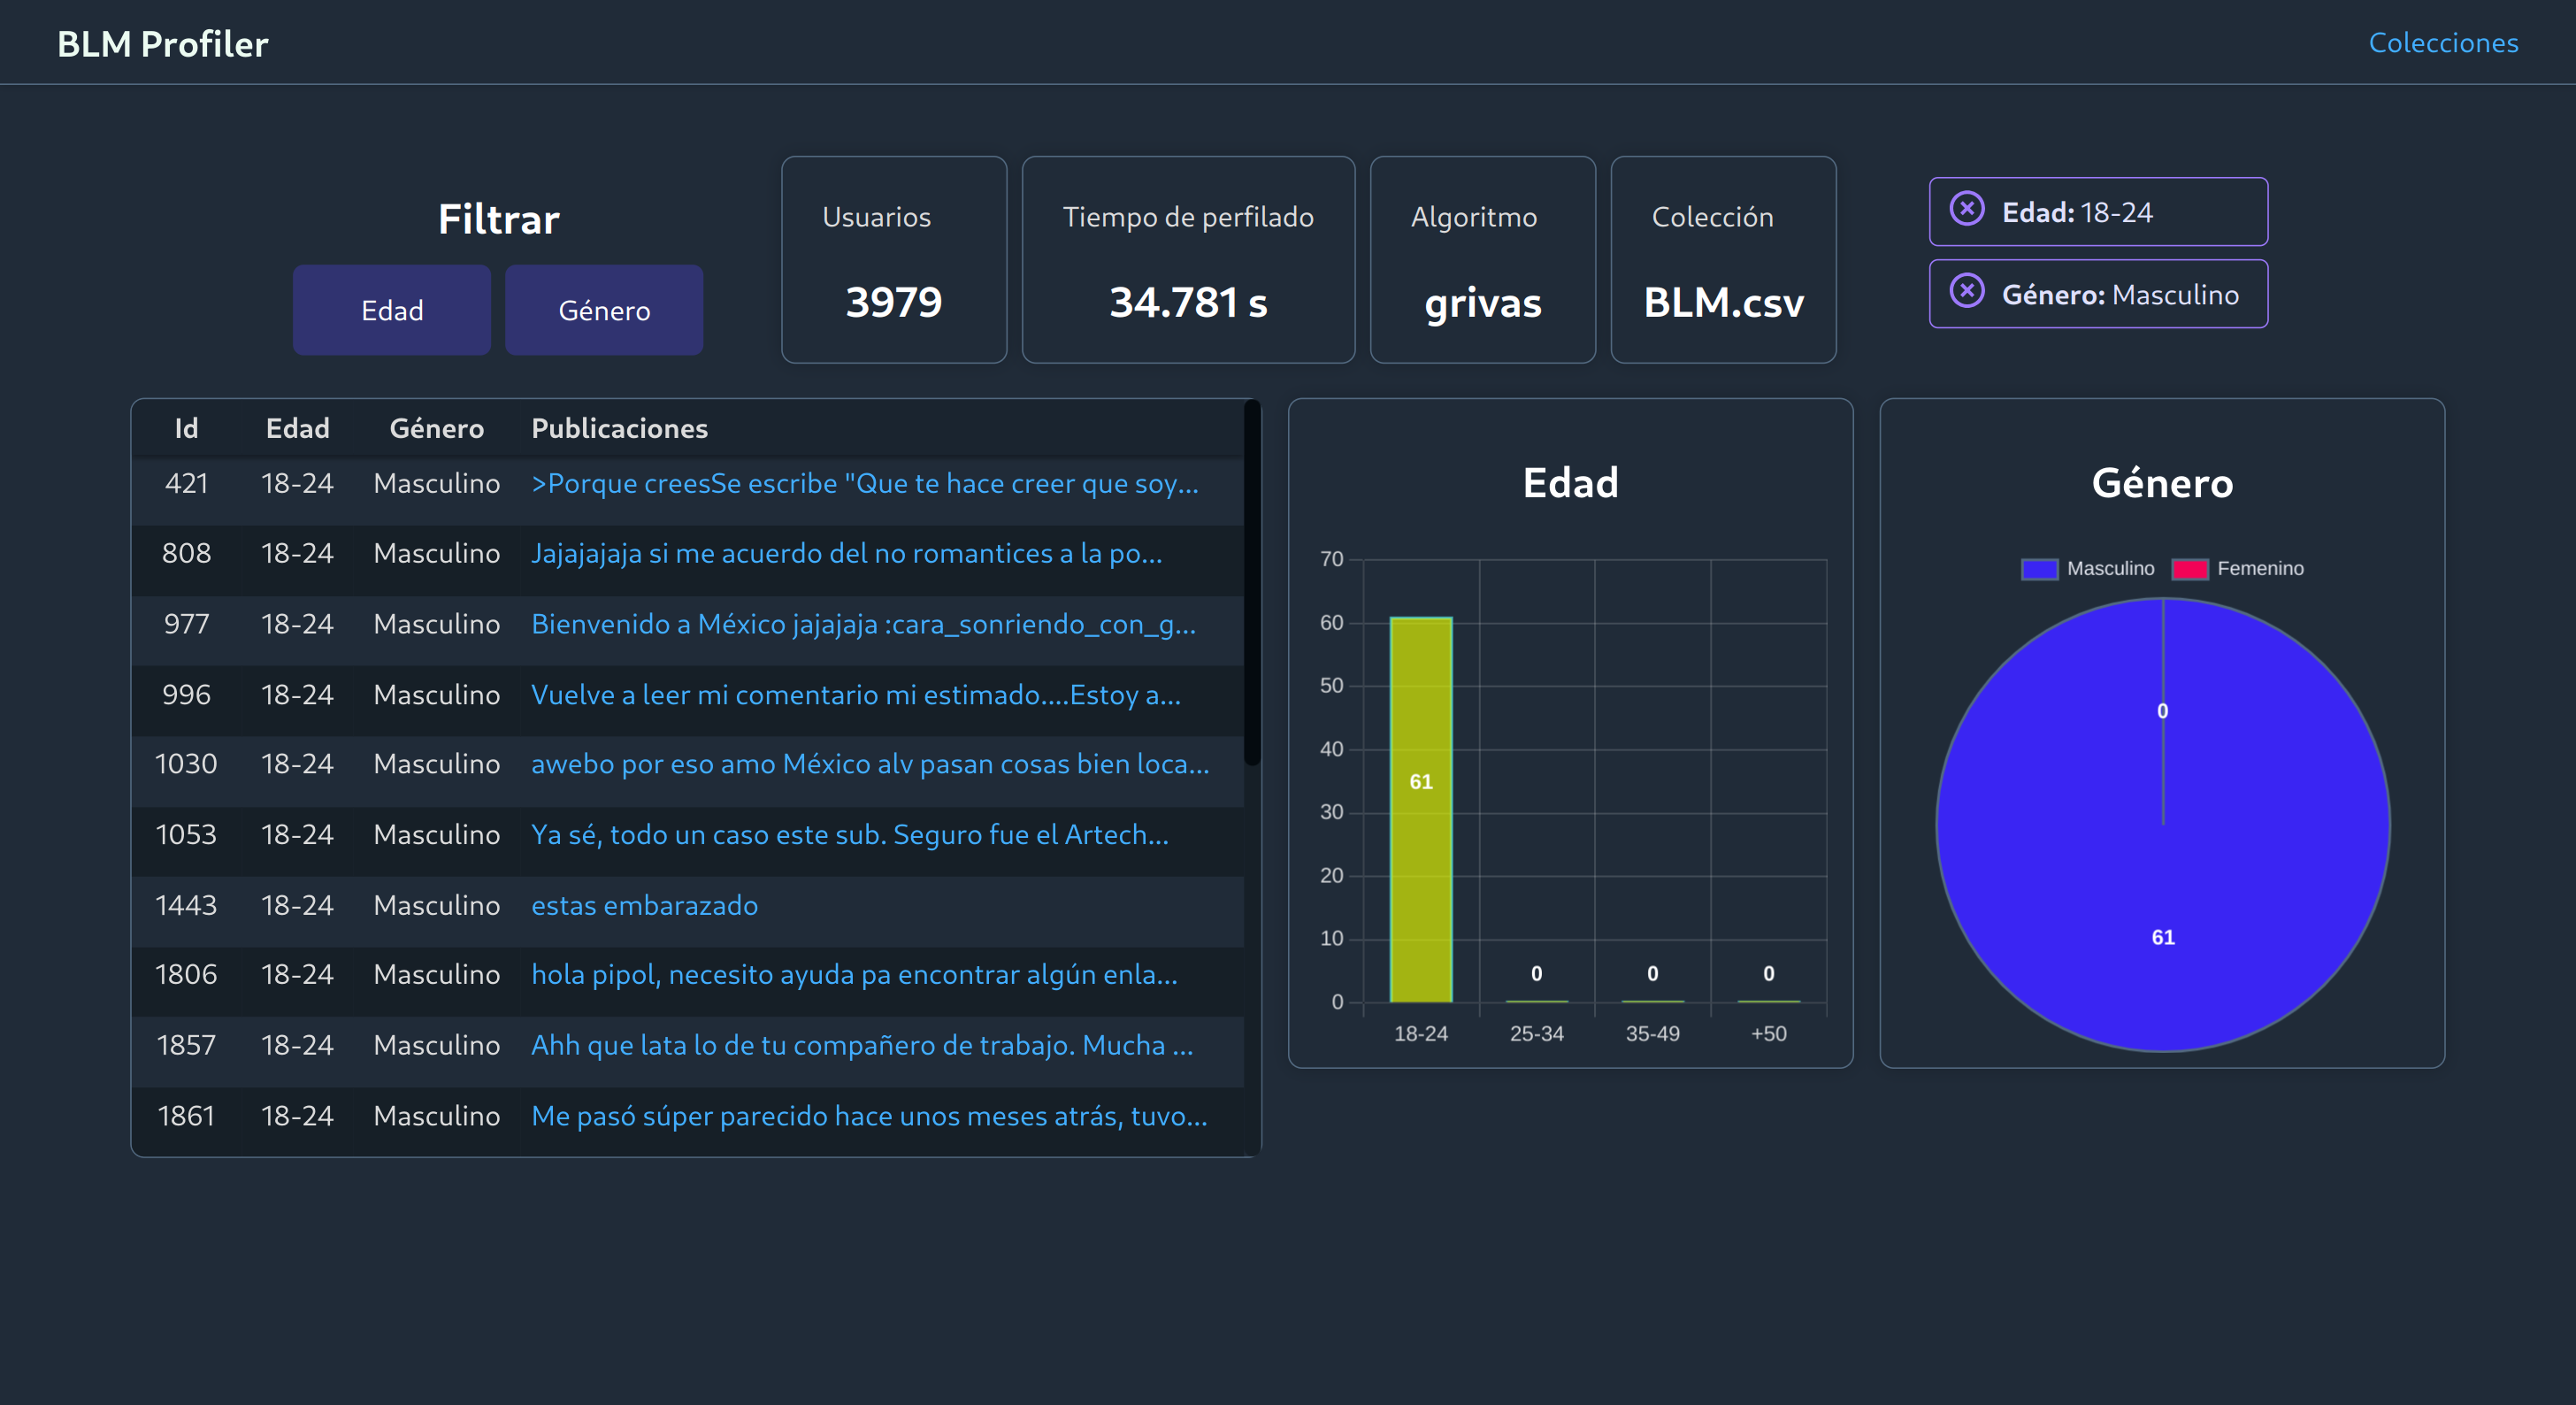
\includegraphics[width=\textwidth]{imaxes/capturas-app/desktop/dashboard-perfilado-edad-genero.png}
  \caption{\textit{Desktop}} 
  \end{subfigure}
  \begin{subfigure}{0.223\textwidth}
   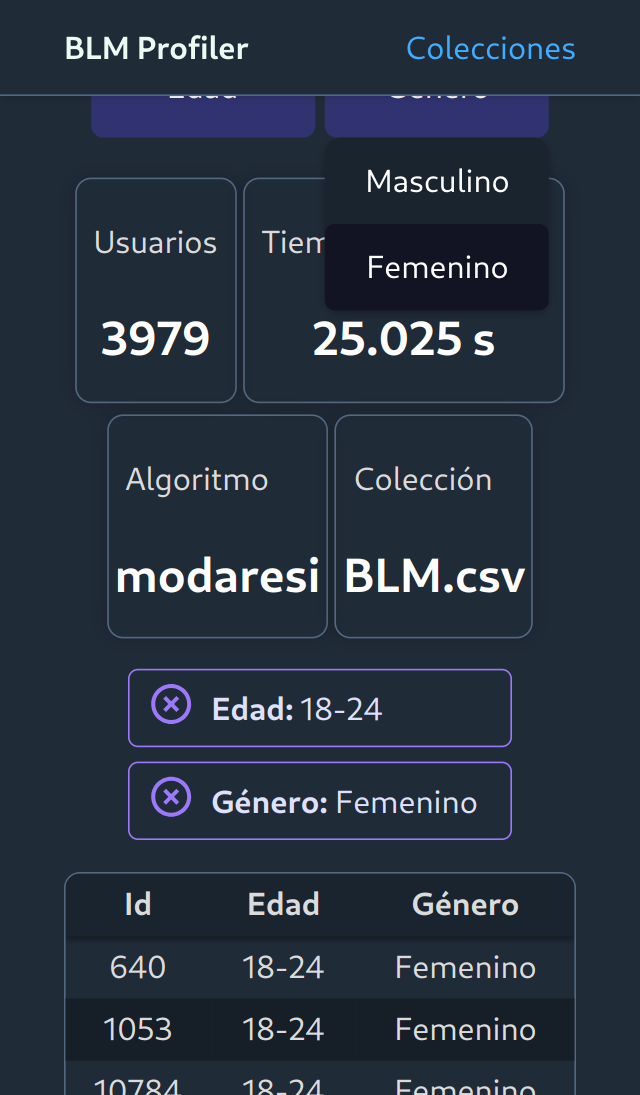
\includegraphics[width=\textwidth]{imaxes/capturas-app/mobile/dashboard-filtrado-edad-genero.png}
  \caption{\textit{Mobile}} 
  \end{subfigure}
  \caption{\textit{Dashboard} de la colección perfilada filtrado por género y edad.}
  \label{fig:app/dashboard-filtered-edad-genero}
\end{figure}

\subsection{Publicaciones de un usuario}
Por ejemplo, si deseáramos examinar el estilo de redacción de un usuario masculino de entre 25 a 34 años, haríamos clic sobre el enlace de la columna <<Publicaciones>> en la versión \textit{desktop}, o directamente seleccionando una fila de la tabla, en la versión \textit{mobile}. Con esta acción podríamos ver las publicaciones del usuario seleccionado en una página similar a la de la figura \ref{fig:app/user-info}.

\begin{figure}[H]
  \centering
  \begin{subfigure}{0.7\textwidth}
   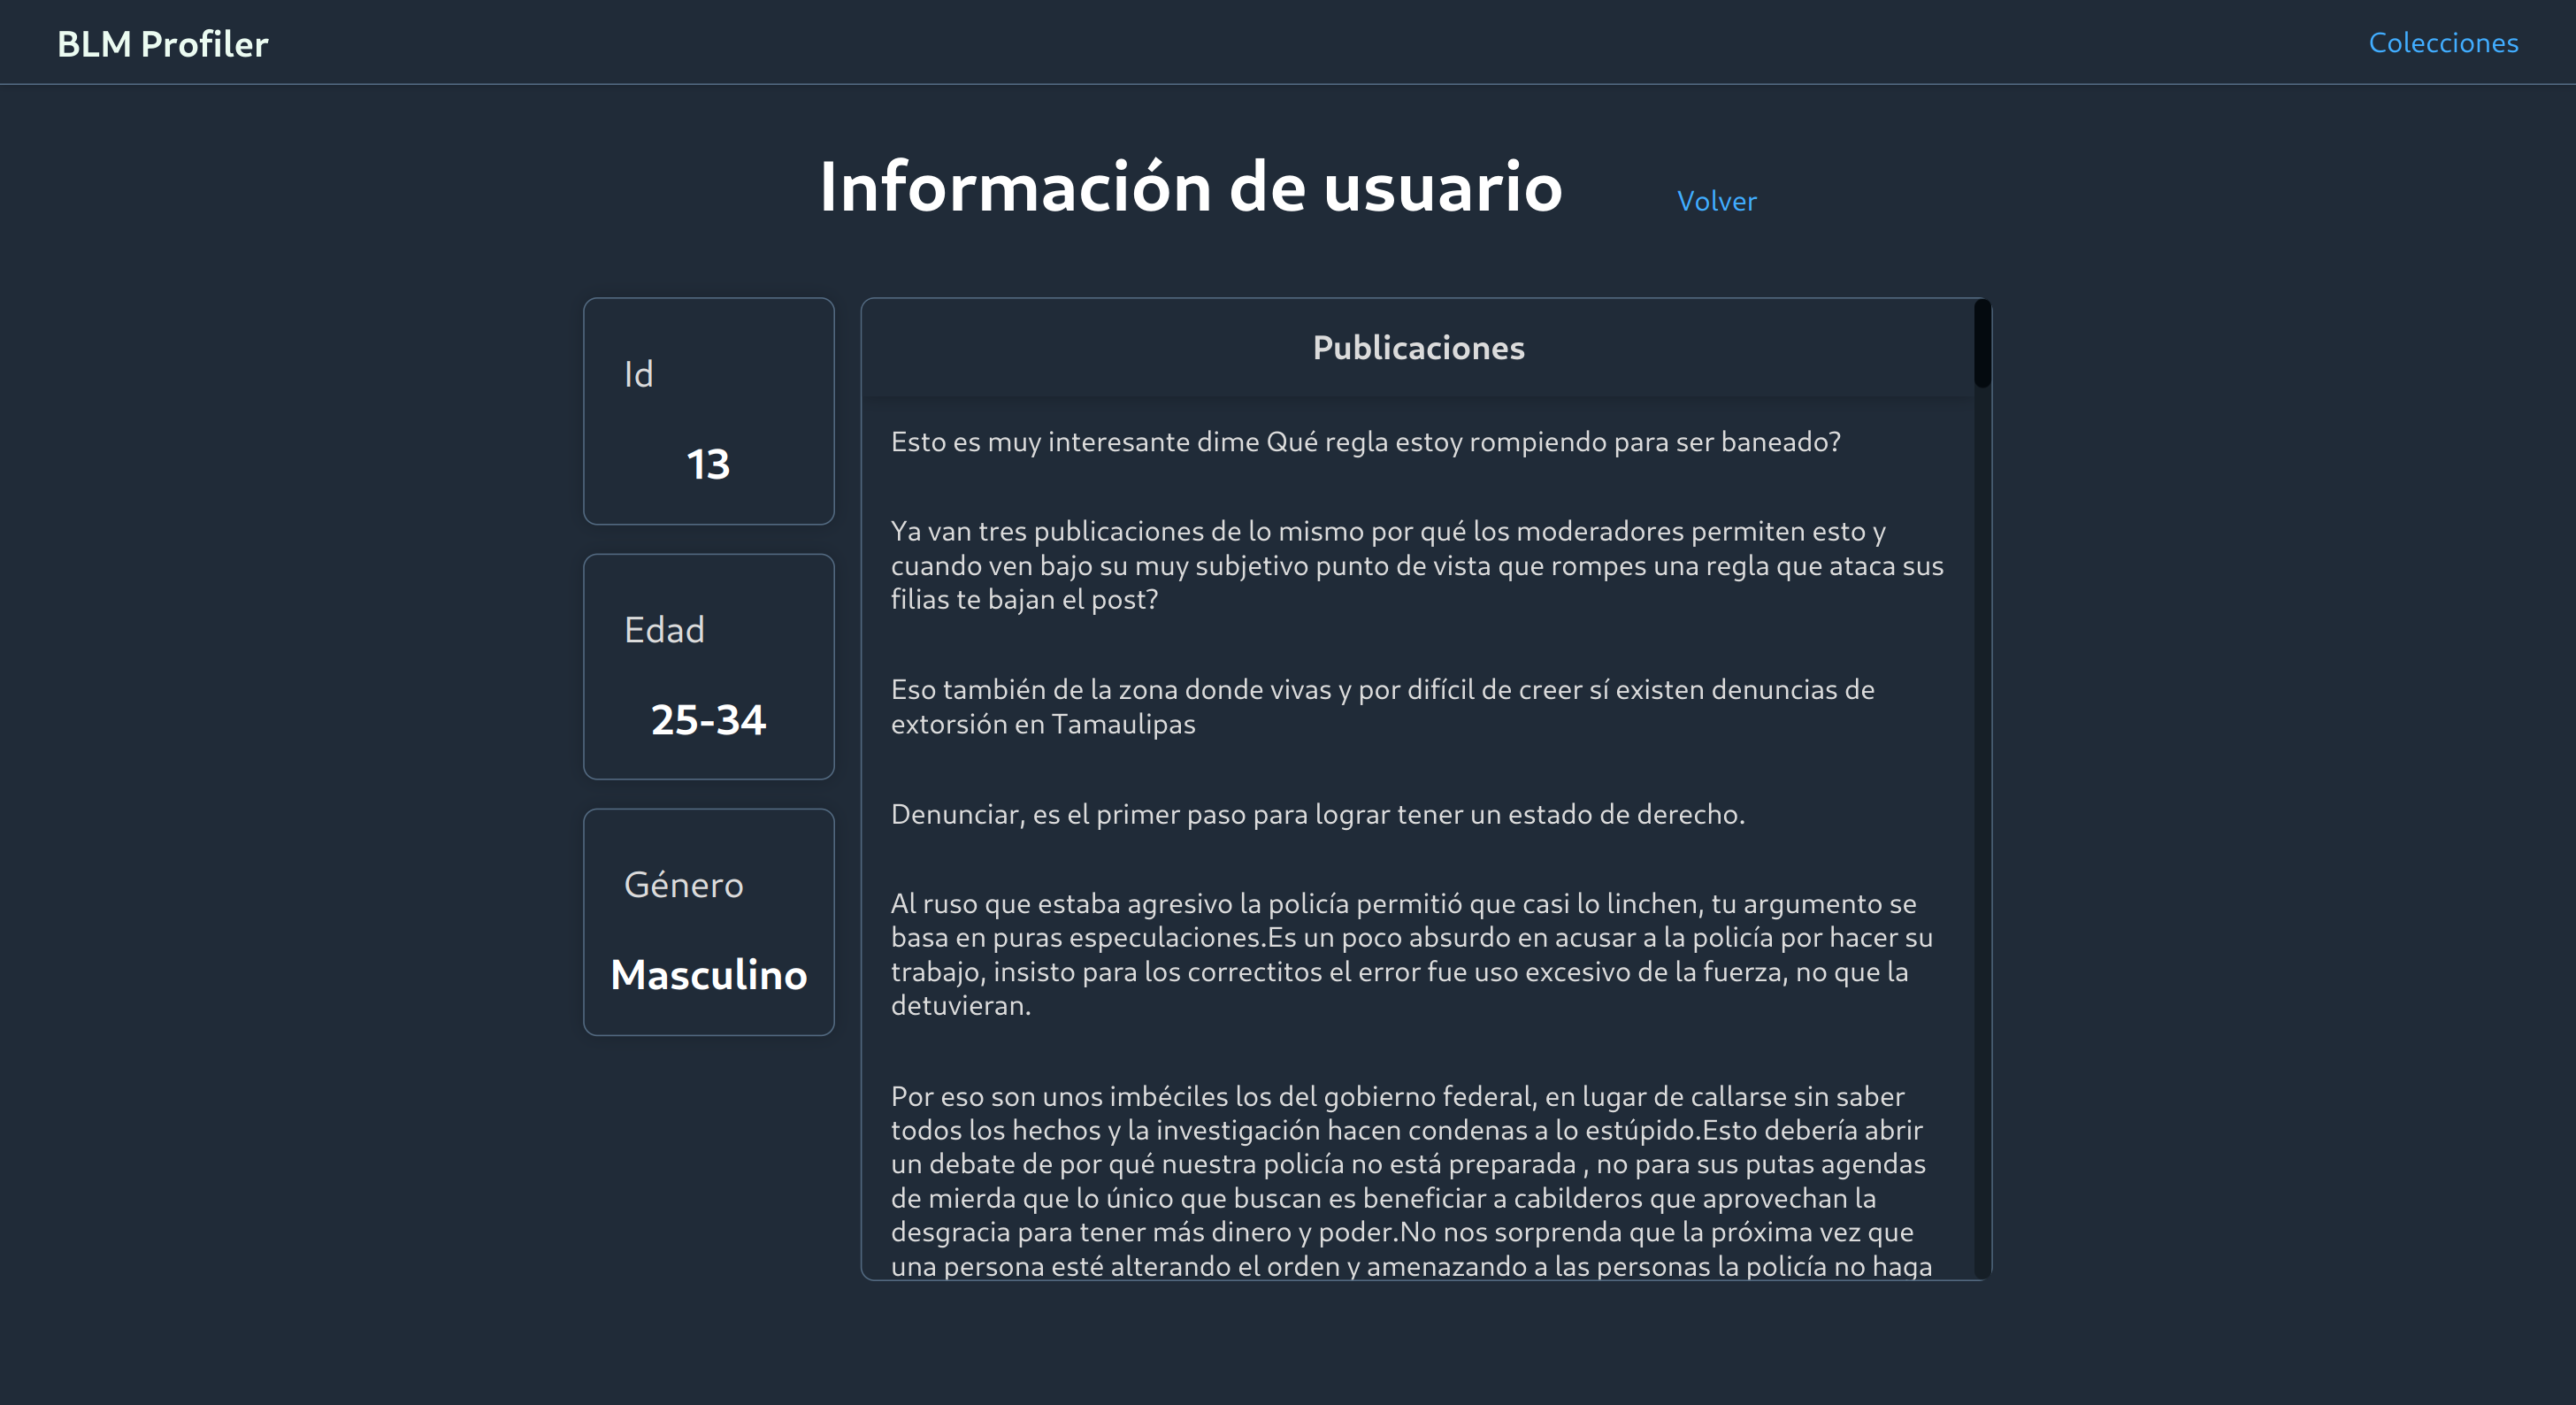
\includegraphics[width=\textwidth]{imaxes/capturas-app/desktop/info-usuario.png}
  \caption{\textit{Desktop}} 
  \end{subfigure}
  \begin{subfigure}{0.223\textwidth}
   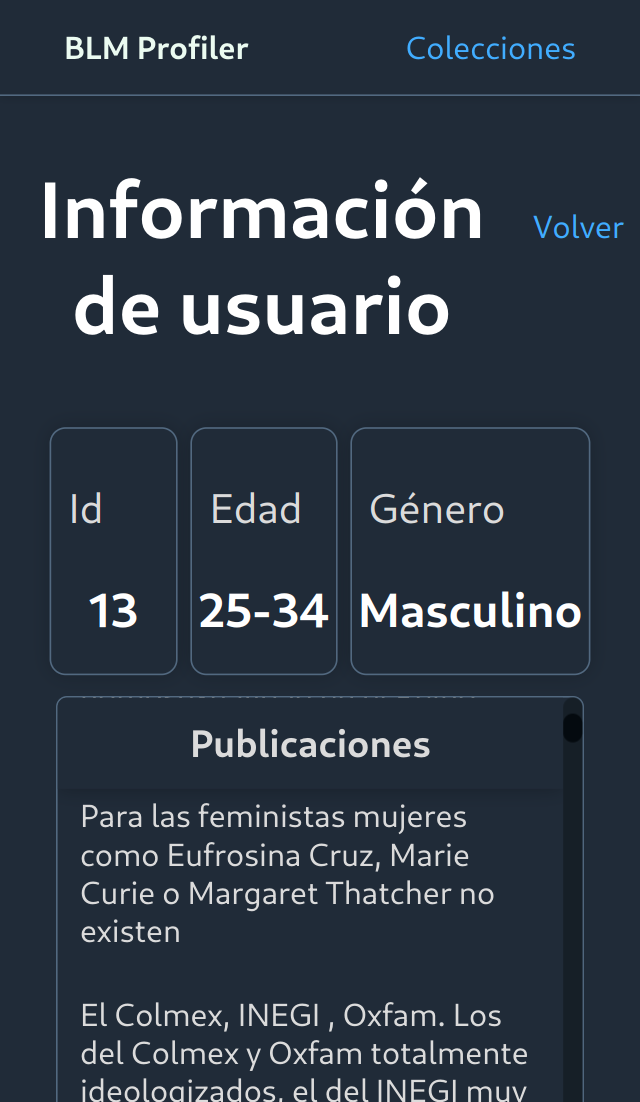
\includegraphics[width=\textwidth]{imaxes/capturas-app/mobile/info-usuario.png}
  \caption{\textit{Mobile}} 
  \end{subfigure}
  \caption{Página de la vista en detalle de un usuario de la colección.}
  \label{fig:app/user-info}
\end{figure}

\subsection{Listado de colecciones}
En cambio, si no deseamos perfilar una colección nueva sino que queremos ver el listado histórico de colecciones ya perfiladas, en la barra de navegación tenemos un enlace, arriba a la derecha, llamado <<Colecciones>> que nos llevará a una página como la de la figura \ref{fig:app/colecciones}. 

\begin{figure}[H]
  \centering
  \begin{subfigure}{0.7\textwidth}
   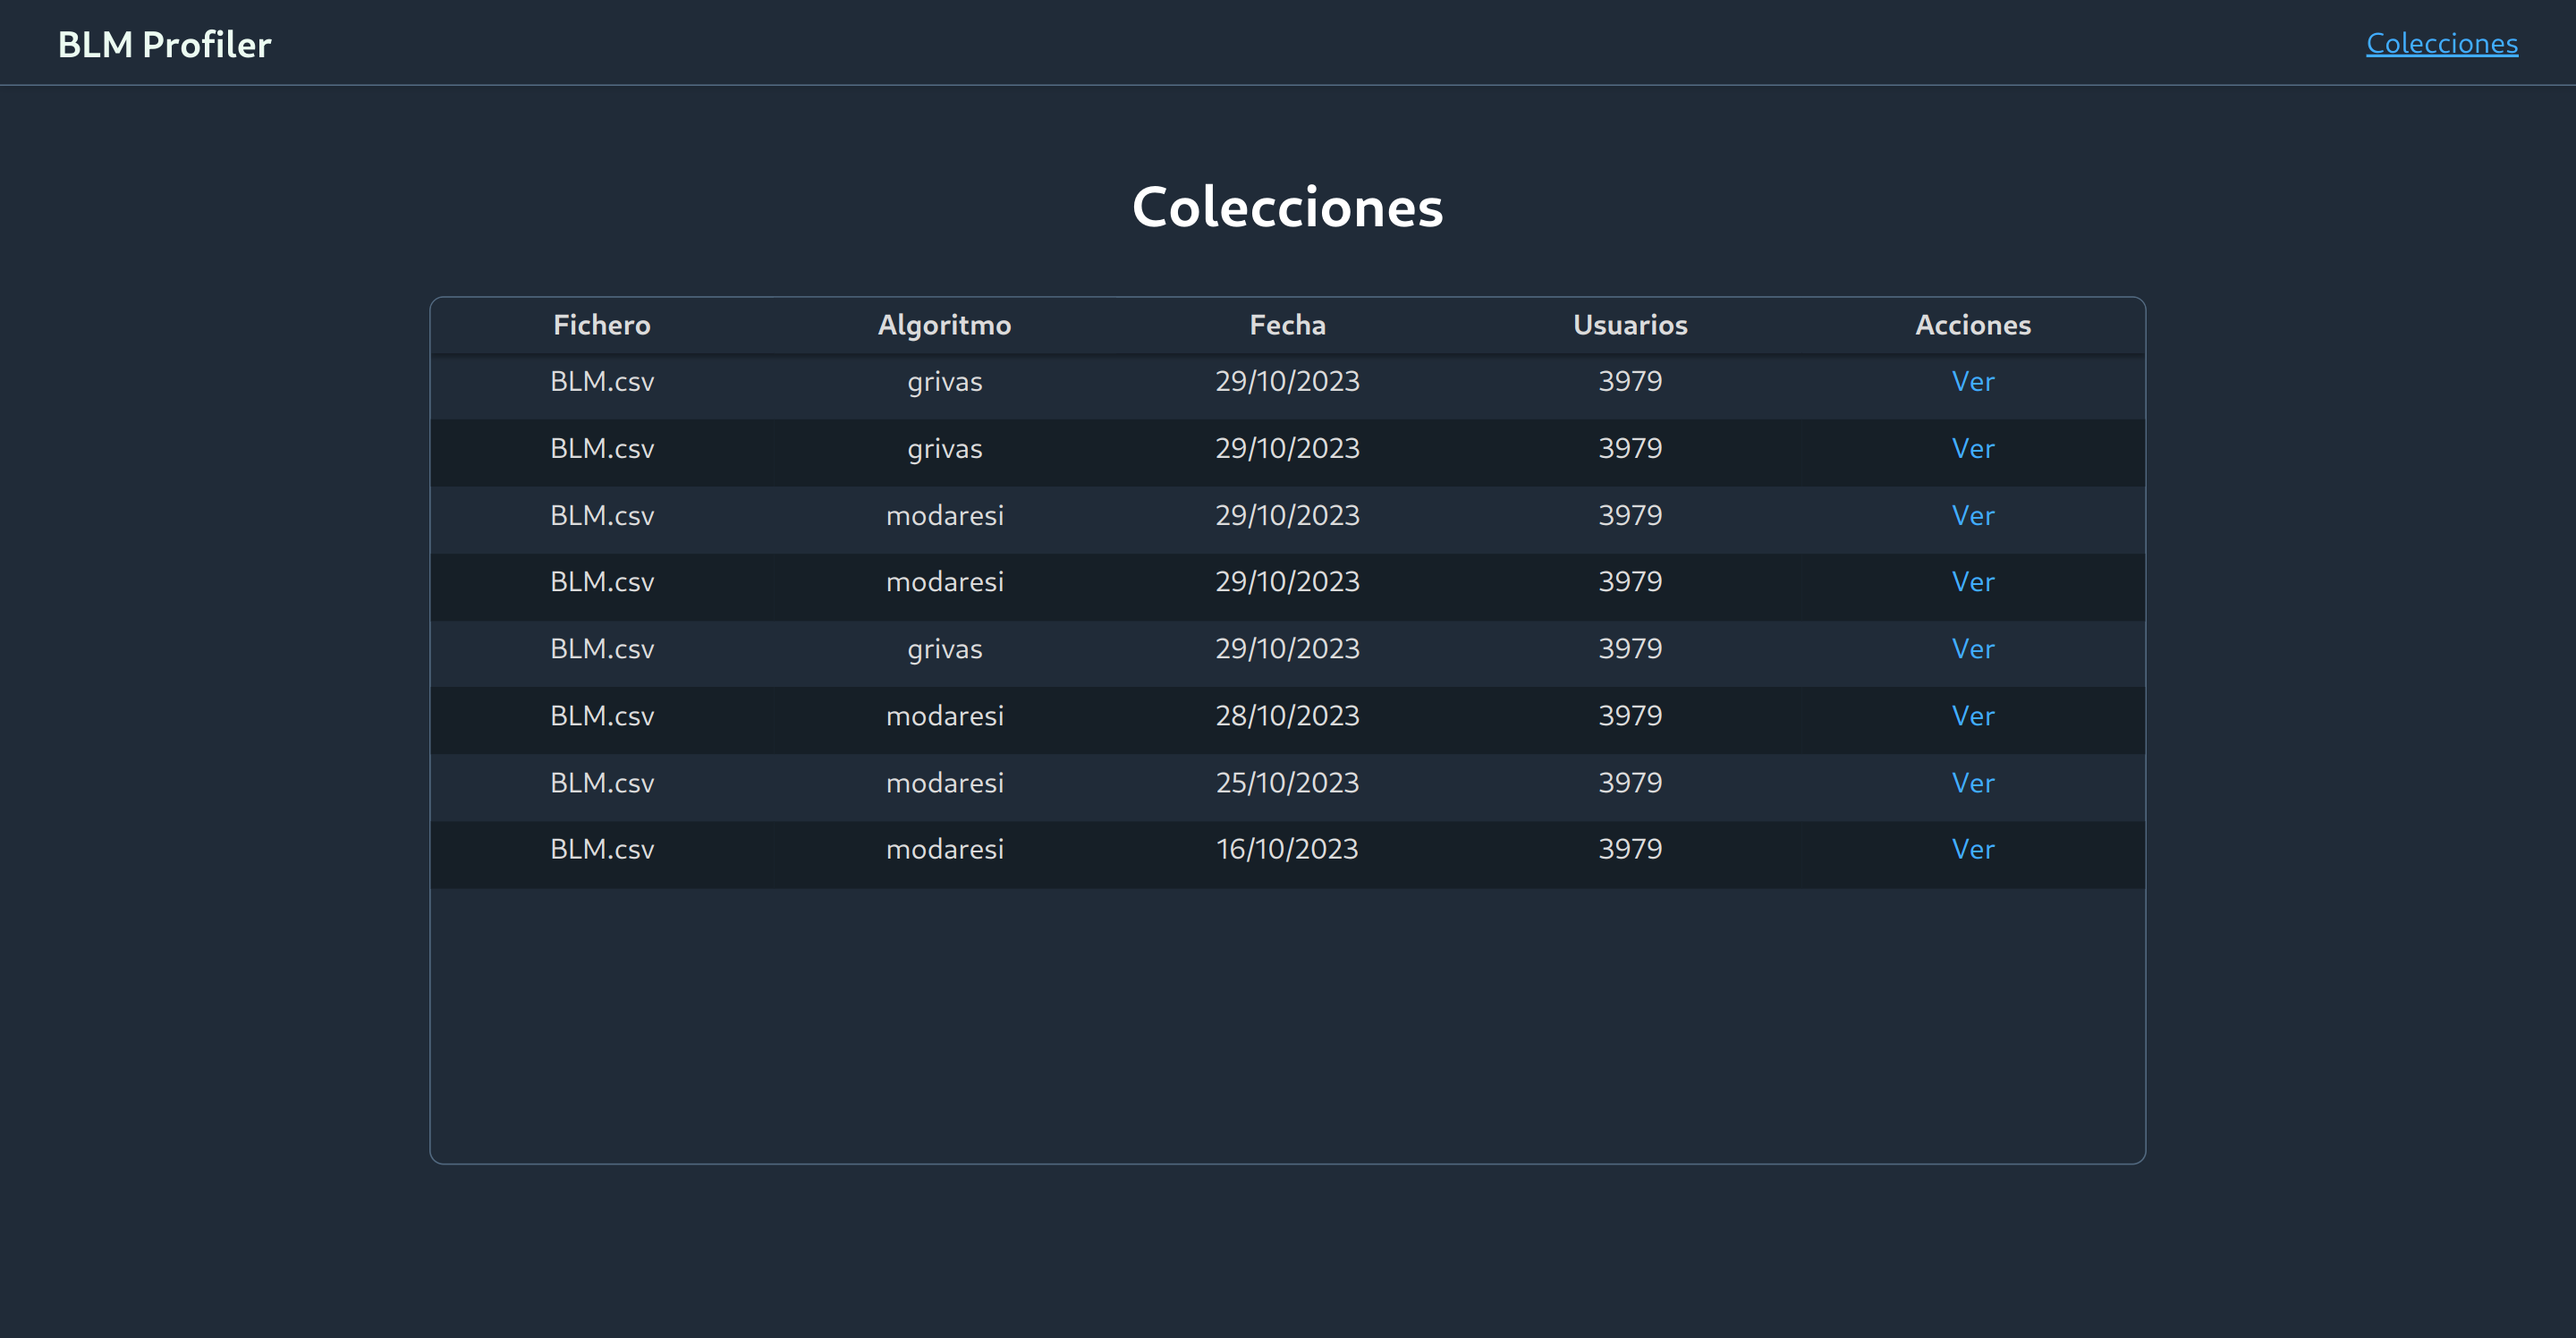
\includegraphics[width=\textwidth]{imaxes/capturas-app/desktop/colecciones.png}
  \caption{\textit{Desktop}} 
  \end{subfigure}
  \begin{subfigure}{0.2115\textwidth}
   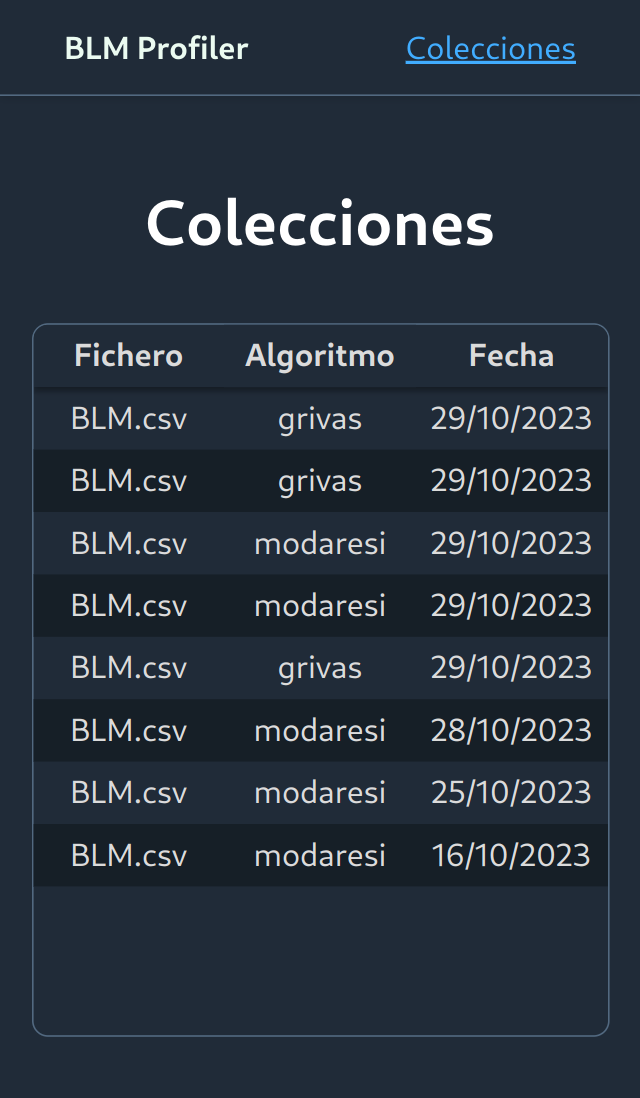
\includegraphics[width=\textwidth]{imaxes/capturas-app/mobile/colecciones.png}
  \caption{\textit{Mobile}} 
  \end{subfigure}
  \caption{Página donde se puede ver el listado de colecciones perfiladas.}
  \label{fig:app/colecciones}
\end{figure}

En esta, tendremos una tabla con las colecciones perfiladas, ordenadas cronológicamente de más a menos recientes. También podremos ver detalles como el nombre del fichero subido, la fecha de subida y el número de usuarios de la colección y algoritmo de perfilado usado en el caso de la versión \textit{desktop}. Asimismo en la columna <<Acciones>> hay un enlace llamado <<Ver>> que nos dirigirá a la página del \textit{dashboard} de esa colección. En la versión \textit{mobile} se puede navegar al \textit{dashboard} tocando sobre la fila de la colección que queramos ver.

\section{Análisis de resultados}

Tras haber explorado el funcionamiento e interfaz de la herramienta de perfilado desarrollada, se procede a una segunda fase en la que se analizan y discuten los resultados obtenidos mediante su uso.

Esta sección se dividirá en un apartado por cada \textit{profiler} utilizado, así como un apartado final a modo de conclusiones generales sobre los resultados de ambos.

Como ya hemos comentado anteriormente en el capítulo \ref{chap:desarrollo}, no hemos incluido finalmente la funcionalidad de perfilado mediante el algoritmo de \citet{loscalis22} explicado en el apartado \ref{subsec:1aprox}, debido al pobre rendimiento del mismo y en mayor medida a la falta de hardware especializado de nuestra máquina local. Por este motivo tampoco hemos analizado los resultados del mismo en esta sección.

\subsection{Algoritmo de \citet{modaresi:2016}}
Vamos a comenzar viendo en detalle los resultados del perfilado mediante el algoritmo de \cite{modaresi:2016}, visto en detalle en \ref{subsec:3aprox}.

En cuestión de edad, se pueden observar las distribuciones de edad obtenidas  por género en la figura \ref{fig:blm/resultados-edad-moda}. Lo primero que llama la atención, es el gran desequilibrio de usuarios en favor del grupo de 25-34 años, el cual supone prácticamente la totalidad de los mismos, un 99.55\% de la colección. Mientras que, los grupos de entre 18-24 y 35-49 solo alcanzan 9 usarios cada uno (menos del 0.3\%) y el grupo de mayores de 50 años se queda vacío. En las distribuciones de usuarios por género se mantiene constante esta tendencia.

\begin{figure}[H]
  \centering
  \begin{subfigure}{0.3\textwidth}
   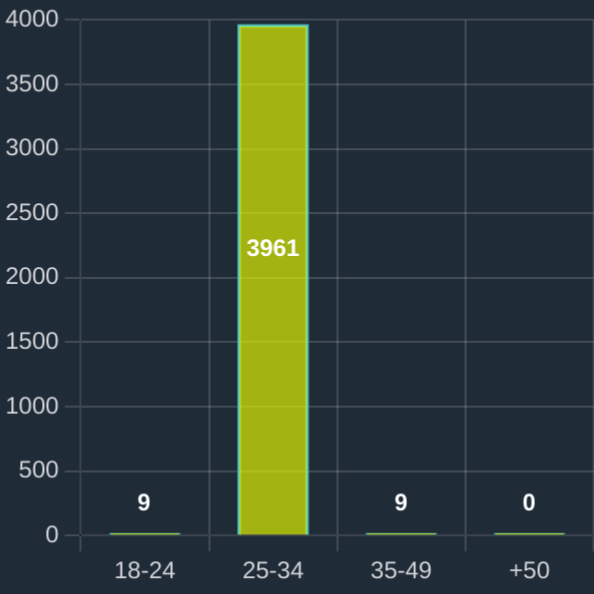
\includegraphics[width=\textwidth]{imaxes/capturas-app/graficos/modaresi/grafico-edad-moda.png}
  \caption{Edad (ambos géneros)}
  \label{subfig:blm/resultados-edad-moda}
  \end{subfigure}
  \begin{subfigure}{0.3\textwidth}
   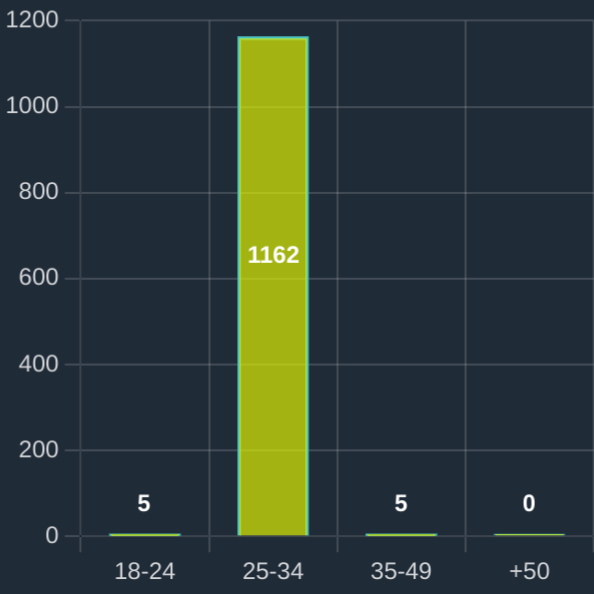
\includegraphics[width=\textwidth]{imaxes/capturas-app/graficos/modaresi/grafico-edad-moda-fem.png}
  \caption{Edad (usuarios femeninos)} 
  \end{subfigure}
  \begin{subfigure}{0.3\textwidth}
   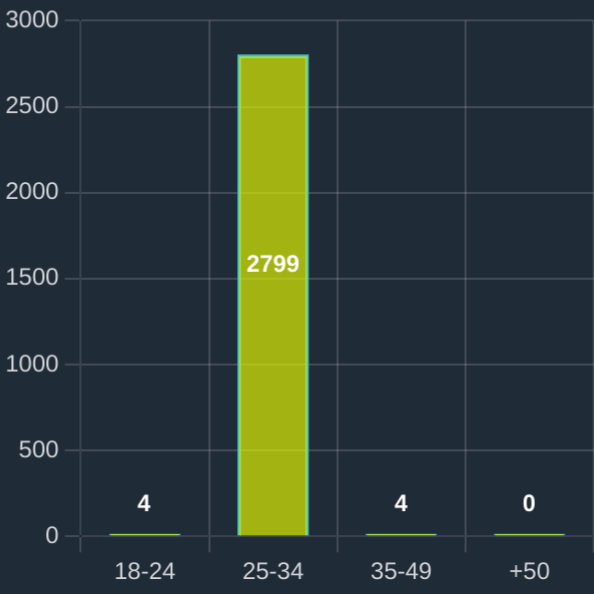
\includegraphics[width=\textwidth]{imaxes/capturas-app/graficos/modaresi/grafico-edad-moda-masc.png}
  \caption{Edad (usuarios masculinos)} 
  \end{subfigure}
  \caption{Distribuciones de edad obtenidas mediante algoritmo de \citet{modaresi:2016}, en corpus \acrshort{blm} en español, según género de usuarios.}
  \label{fig:blm/resultados-edad-moda}
\end{figure}

En cuestión de género, se puede ver en el gráfico en forma de tarta de la figura \ref{fig:blm/resultados-genero-moda} que los usuarios masculinos que publicaban en \acrshort{blm} constituyen casi tres cuartas partes del total de la colección (70.54\%). Sin embargo, si vemos los gráficos por edades podemos darnos cuenta que este desequilibrio solo se da en el rango de edad de entre 25 y 34 años, ya que en el de 18-24 y 35-49 los usuarios femeninos representan más de la mitad en esos grupos demográficos. No obstante, al haber un desequilibro tan grande en cuestión de edad estas mayorías no tienen apenas repercusión en los usuarios totales.

\begin{figure}[H]
  \centering
  \begin{subfigure}{0.3\textwidth}
   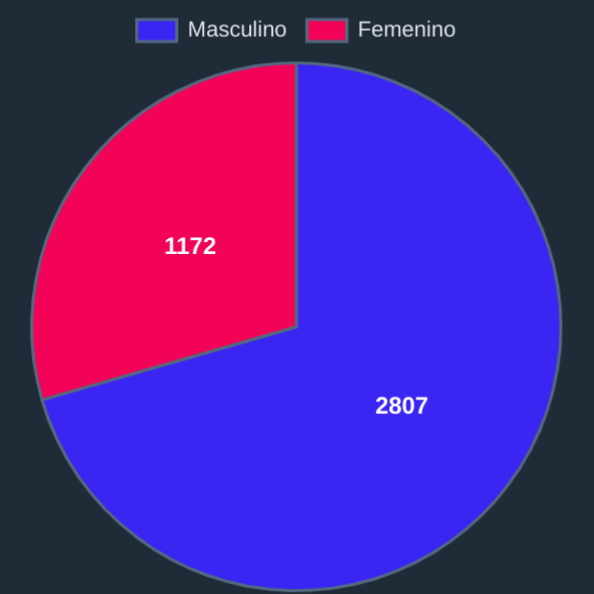
\includegraphics[width=\textwidth]{imaxes/capturas-app/graficos/modaresi/grafico-genero.png}
  \caption{Género (cualquier edad)}
  \label{subfig:blm/resultados-genero-moda}
  \end{subfigure}
  \begin{subfigure}{0.3\textwidth}
   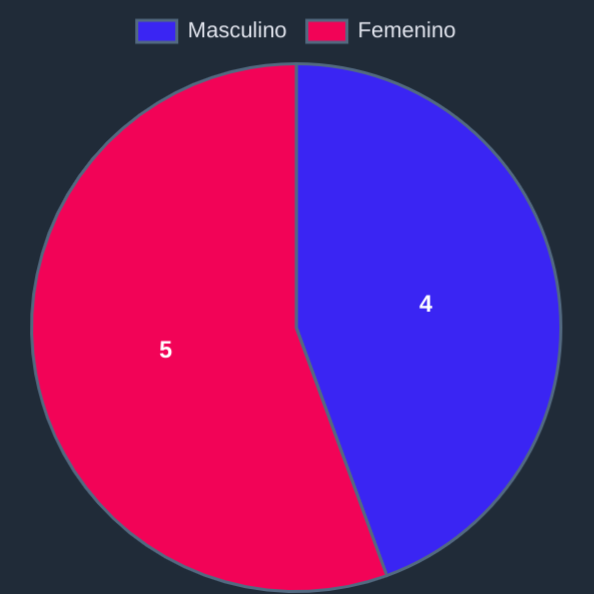
\includegraphics[width=\textwidth]{imaxes/capturas-app/graficos/modaresi/grafico-genero-jj.png}
  \caption{Géner (18-24 años)}
  \end{subfigure}
  \begin{subfigure}{0.3\textwidth}
   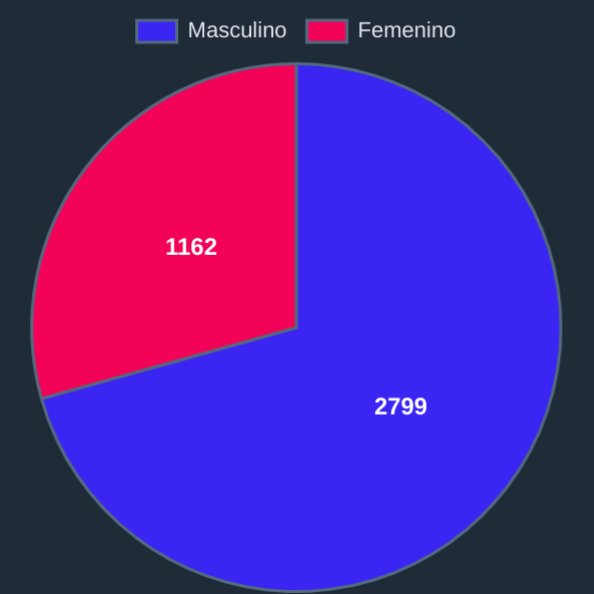
\includegraphics[width=\textwidth]{imaxes/capturas-app/graficos/modaresi/grafico-genero-j.png}
  \caption{Género (25-34 años)}
  \end{subfigure}
  \begin{subfigure}{0.3\textwidth}
   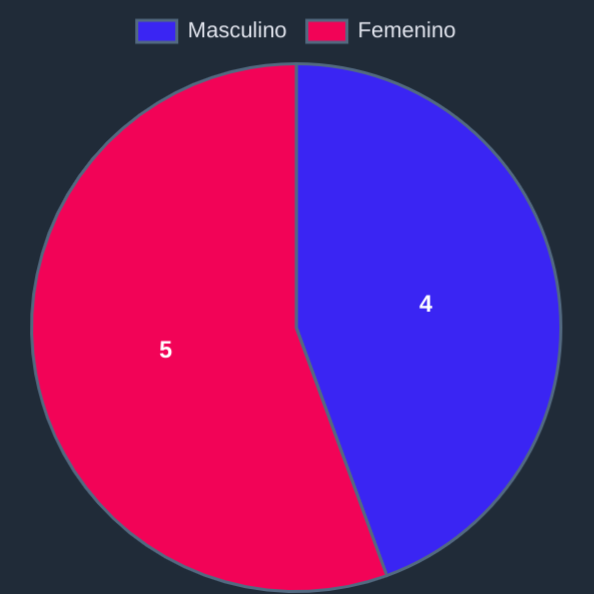
\includegraphics[width=\textwidth]{imaxes/capturas-app/graficos/modaresi/grafico-genero-v.png}
  \caption{Género (35-49 años)}
  \end{subfigure}
  \begin{subfigure}{0.3\textwidth}
   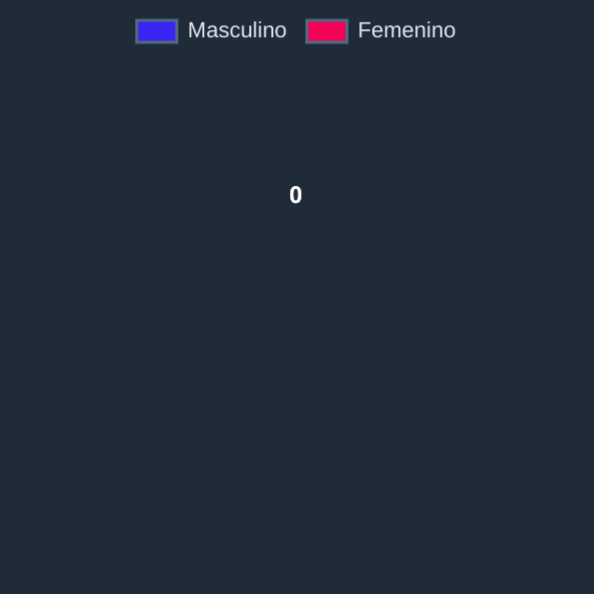
\includegraphics[width=\textwidth]{imaxes/capturas-app/graficos/modaresi/grafico-genero-vv.png}
  \caption{Género (+50 años)}
  \end{subfigure}
  \caption{Distribuciones de género obtenidas mediante algoritmo de modaresi \cite{modaresi:2016}, sobre corpus \acrshort{blm} en español, según rango de edad de usuarios.}
  \label{fig:blm/resultados-genero-moda}
\end{figure}

A modo de resumen, en la tabla \ref{tab:blm/results-moda} se pueden visualizar con detalle la distribución de usuarios en estas dos categorías. Como se podía intuir el grupo demográfico más numeroso es el de usuarios masculinos entre 25-34 años de edad (70.34\%), seguido por las usuarias femeninas de ese mismo grupo cronológico (29.20\%). Otro aspecto resaltable, es la ausencia de usuarios mayores de 50 años.

\begin{table}[H]
    \centering
    \rowcolors{2}{white}{udcgray!25}
    {
    \setlength{\tabcolsep}{0.6\tabcolsep}
    \begin{tabular}{|c|c|c|c|c|c|}
        \hline
        \rowcolor{udcpink!25}
        \diagbox{\textbf{Género}}{\textbf{Edad}} & \textbf{18-24} & \textbf{25-34} & \textbf{35-49} & \textbf{+50} & \textbf{Total} \\ \hline
        \textbf{Femenino} & 5 & 1162 & 5 & 0 & 1172 \\ \hline
        \textbf{Masculino} & 4 & 2799 & 4 & 0 & 2807 \\ \hline
        \textbf{Total} & 9 & 3961 & 9 & 0 & 3979 \\ \hline

    \end{tabular}%
    }
    \caption{Tabla resumen de los usuarios de la colección \acrshort{blm} perfilados mediante algoritmo de \citet{modaresi:2016}.}
    \label{tab:blm/results-moda}
\end{table}

\subsection{Algoritmo de \citet{grivas2015author}}
A continuación se exponen en detalle los resultados obtenidos aplicando el algoritmo de \citet{grivas2015author}, analizado en el apartado \ref{subsec:2aprox} de la memoria.

Comenzando otra vez con la categoría de edad, podemos contemplar de nuevo en la figura \ref{fig:blm/resultados-edad-grivas}, como, aunque ligeramente menor que antes, la gran disparidad de usuarios se mantiene en favor del grupo entre 25-34 años, que aglutina el 97.49\% de la colección. En este caso es el grupo más joven (18-24 años) el siguiente más numeroso con el 2.31\%. Mientras que, de nuevo los grupos de usuarios más mayores, 35-49 y +50 se quedan casi vacíos con 3 y 5 usuarios cada uno. Al examinar estos rangos según el género, se puede apreciar como los usuarios femeninos están bastante más equilibrados, en cuanto a que el grupo de 18-24 representa un mayor porcentaje respecto al total que en el caso masculino (16.67\% por 1.60\%).

\begin{figure}[H]
  \centering
  \begin{subfigure}{0.3\textwidth}
   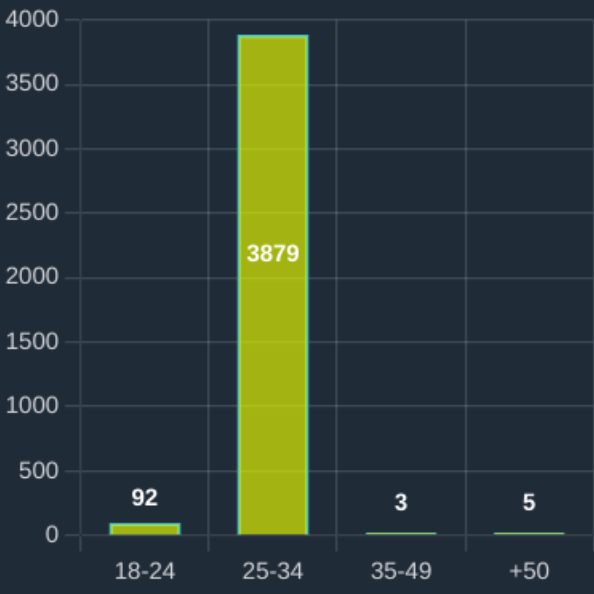
\includegraphics[width=\textwidth]{imaxes/capturas-app/graficos/grivas/grafico-edad-grivas.png}
  \caption{Edad (ambos géneros)} 
  \end{subfigure}
  \begin{subfigure}{0.3\textwidth}
   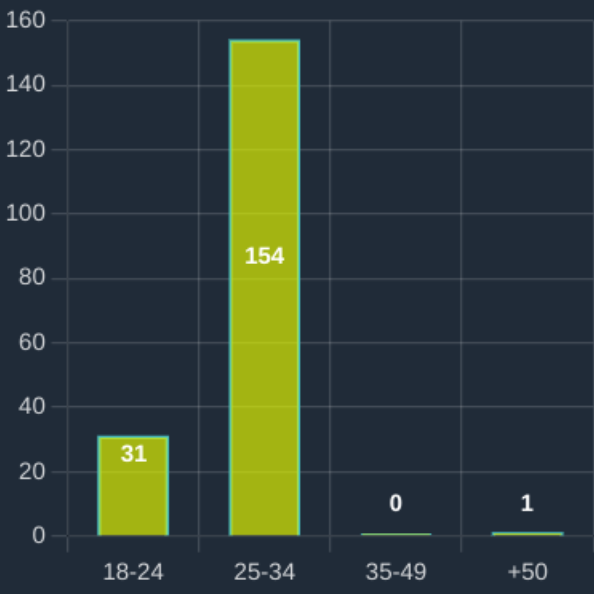
\includegraphics[width=\textwidth]{imaxes/capturas-app/graficos/grivas/grafico-edad-grivas-femenino.png}
  \caption{Edad (usuarios femeninos)} 
  \end{subfigure}
  \begin{subfigure}{0.3\textwidth}
   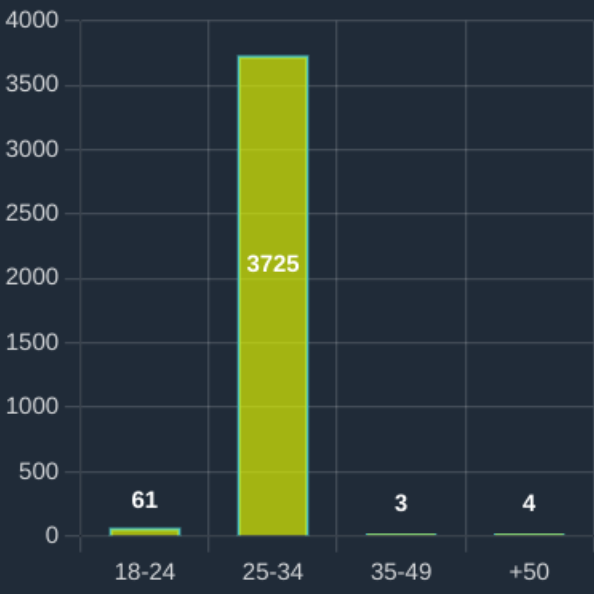
\includegraphics[width=\textwidth]{imaxes/capturas-app/graficos/grivas/grafico-edad-grivas-masculino.png}
  \caption{Edad (usuarios masculinos)} 
  \end{subfigure}
  \caption{Distribuciones de edad obtenidas mediante algoritmo de \citet{grivas2015author}, en corpus \acrshort{blm} en español, según género de usuarios.}
  \label{fig:blm/resultados-edad-grivas}
\end{figure}

Siguiendo con el género, en este caso se puede ver (figura \ref{fig:blm/resultados-genero-grivas}) una mayoría masculina aún más pronunciada que con el algoritmo de modaresi, siendo estos el 95.32\% de la colección. Por grupos de edad se mantiene más o menos igual esta gran mayoría, a excepción del grupo más joven (18-24 años) donde el porcentaje de usuarias crece de el 5 al 33.70\%.
\begin{figure}[H]
  \centering
  \begin{subfigure}{0.3\textwidth}
   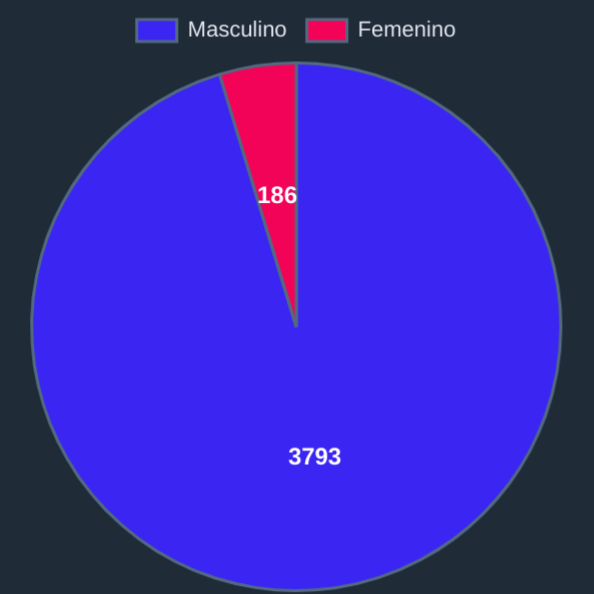
\includegraphics[width=\textwidth]{imaxes/capturas-app/graficos/grivas/grafico-genero.png}
  \caption{Género (cualquier edad)}
  \label{subfig:blm/resultados-genero-grivas}
  \end{subfigure}
  \begin{subfigure}{0.3\textwidth}
   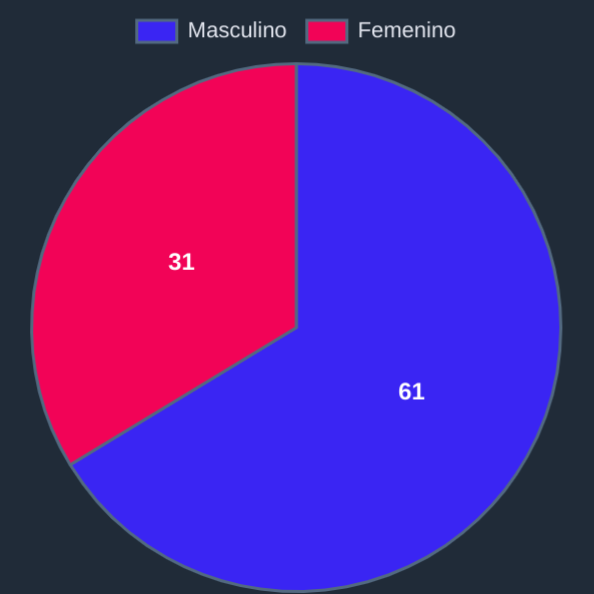
\includegraphics[width=\textwidth]{imaxes/capturas-app/graficos/grivas/grafico-genero-jj.png}
  \caption{Género (18-24 años)}
  \end{subfigure}
  \begin{subfigure}{0.3\textwidth}
   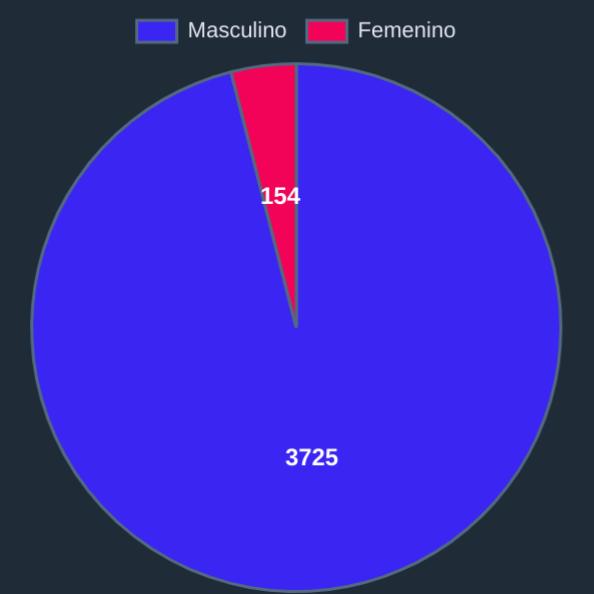
\includegraphics[width=\textwidth]{imaxes/capturas-app/graficos/grivas/grafico-genero-j.png}
  \caption{Género (25-34 años)}
  \end{subfigure}
  \begin{subfigure}{0.3\textwidth}
   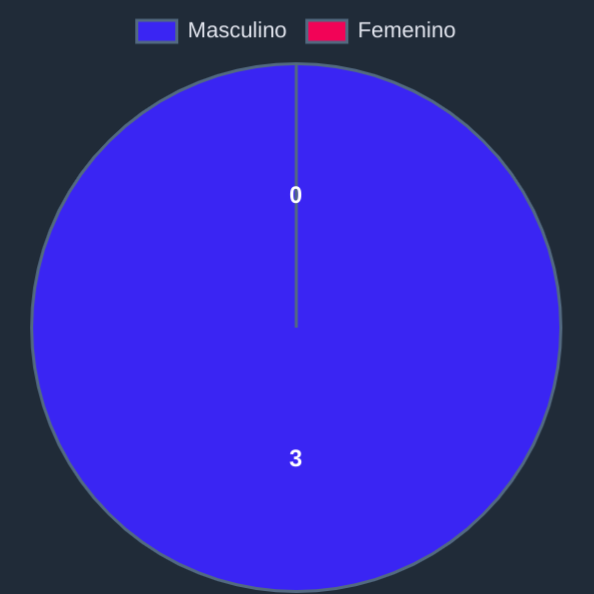
\includegraphics[width=\textwidth]{imaxes/capturas-app/graficos/grivas/grafico-genero-v.png}
  \caption{Género (35-49 años)}
  \end{subfigure}
  \begin{subfigure}{0.3\textwidth}
   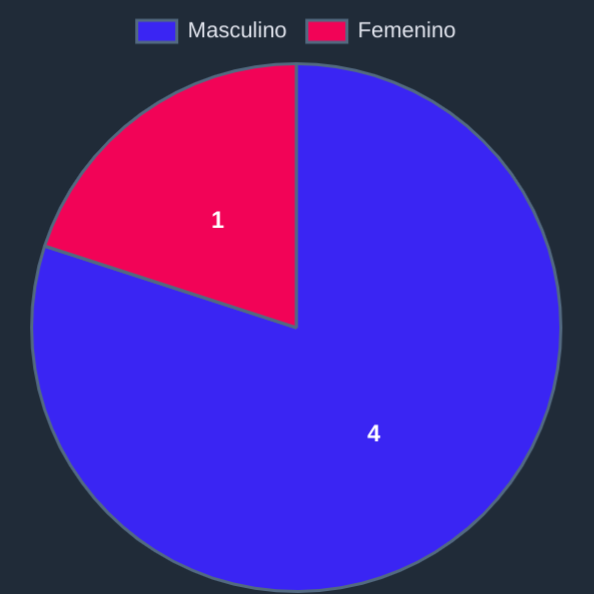
\includegraphics[width=\textwidth]{imaxes/capturas-app/graficos/grivas/grafico-genero-vv.png}
  \caption{Género (+50 años)}
  \end{subfigure}
  \caption{Distribuciones de género obtenidas mediante algoritmo de \citet{grivas2015author}, sobre corpus \acrshort{blm} en español, según rango de edad de usuarios.}
  \label{fig:blm/resultados-genero-grivas}
\end{figure}

Para terminar con este apartado, podemos observar las cifras concretas de usuarios pertenecientes a cada categoría en la tabla \ref{tab:blm/results-grivas}. Como ya adelantábamos, los usuarios masculinos entre 25-34 años predominan en la colección con el 95.38\% seguidos de los femeninos en ese mismo grupo de edad (3.87\%).
\begin{table}[H]
    \centering
    \rowcolors{2}{white}{udcgray!25}
    {
    \setlength{\tabcolsep}{0.6\tabcolsep}
    \begin{tabular}{|c|c|c|c|c|c|}
        \hline
        \rowcolor{udcpink!25}
        \diagbox{\textbf{Género}}{\textbf{Edad}} & \textbf{18-24} & \textbf{25-34} & \textbf{35-49} & \textbf{+50} & \textbf{Total} \\ \hline
        \textbf{Femenino} & 31 & 154 & 0 & 1 & 186 \\ \hline
        \textbf{Masculino} & 61 & 3725 & 3 & 4 & 3793 \\ \hline
        \textbf{Total} & 92 & 3879 & 3 & 5 & 3979 \\ \hline

    \end{tabular}%
    }
    \caption{Tabla resumen según de los usuarios de la colección \acrshort{blm} perfilados mediante algoritmo de \citet{grivas2015author}.}
    \label{tab:blm/results-grivas}
\end{table}

\subsection{Discusión}
En este apartado se hace una discusión acerca de los resultados obtenidos en los dos apartado anteriores. A la vez, se explican las posibles causas de los mismos, así como las implicaciones y conclusiones que se pueden sacar de ellos.

Para empezar, en cuestión de edad ambas aproximaciones apuntan hacia una conclusión parecida: la edad de casi la totalidad de los usuarios que comentaban en \acrshort{blm} está comprendida entre 25-34 años. Siendo el segundo grupo más numeroso el de 18-24 según el algoritmo de \citet{grivas2015author}. Aunque en este último no coinciden ambos algoritmos, es probable que el desequilibrio en cuestión de edad del \textit{dataset} usado para el entrenamiento (\ref{tab:datasets_edad}), haga que estos estén sesgados hacia los grupos de edad más numerosos (25-34 y 35-49). Teniendo en cuenta este hecho, es posible que el desequilibrio en el entrenamiento afecte más a un algoritmo que otro, y por ese motivo el de \citet{modaresi:2016} produce unos resultados tan homogéneos en cuestión de edad. En este sentido, los resultados obtenidos mediante el primer algoritmo \citet{modaresi:2016} parecen estar más influenciados por este equilibrio que los de \citet{grivas2015author}, siendo este último el que alcanza una mayor precisión en las experimentos realizados en cuanto a edad (\ref{tab:aprox2_results}).

Estas conclusiones ganan mayor peso si tenemos en cuenta algunos estudios estadísticos realizados sobre el uso de Reddit, la red social de la que proviene el corpus perfilado. En estos estudios publicados por \citet{reddit2016} se expone como el 59\% de los usuarios de Reddit que participan en temas de actualidad como noticias o discusiones políticas (como es el movimiento \acrshort{blm}), tienen una edad comprendidad entre 18 y 29 años de edad, habiendo otra gran parte de ellos (33\%) entre 30 y 49 años, dejando solo un 7\% restante de mayores de 50.

Por otro lado, los resultados obtenidos en cuanto a género con ambos métodos también nos dejan una conclusión clara: los usuarios varones son  más numerosos que las usuarias mujeres. En este caso, los resultados del algoritmo con mejor rendimiento en los experimentos realizados (\ref{tab:results_aprox3}), como es el de \citet{modaresi:2016}, son los más balanceados que apuntan a un 70\% de usuarios masculinos por el 95\% de usuarios del algoritmo de \citet{grivas2015author}, que quizás muestre un sesgo en favor de este grupo.

Esta proposición va de nuevo en sintonía con los estudios estadísticos sobre Reddit antes mencionados \citep{reddit2016}. En estos se afirma que: los usuarios que se informan y participan en temas de actualidad en la plataforma están constituidos en un 71\% por hombres por un 29\% de mujeres (una distribución de usuarios extremadamente similar a la obtenida con el primer algoritmo). En la figura \ref{fig:blm/estudio-estadistico}, se puede ver una imagen donde se muestran los datos mencionados sobre usuarios de noticias de \textit{Reddit}.

\begin{figure}[H]
  \centering
  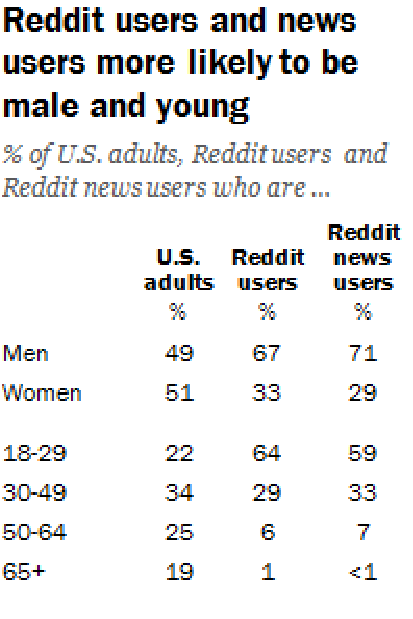
\includegraphics[width=0.3\textwidth]{imaxes/estudio-reddit.pdf}
  \caption{Distribución de usuarios de Reddit según estudio por \citet{reddit2016}.}
  \label{fig:blm/estudio-estadistico}
\end{figure}

En esta línea, podría ser lógico inferir que la distribución de usuarios de Reddit que participan en temas de actualidad, constituya un gran predictivo acerca de la distribución de usuarios en el corpus de referencia.

Por otro lado, un factor importante que limita de manera considerable la fiabilidad de los algoritmos es el hecho de mientras que, la gran mayoría de usuarios tiene pocas publicaciones unos pocos concentran la gran mayoría de \textit{posts} del corpus. En nuestro caso, en el corpus formado por 3979 usuarios, pues 1949 de ellos (el 48.98\% del total) tiene únicamente una publicación en el corpus, 3213 (80\%) tienen menos de 5 publicaciones y 3630 usuarios (más del 90\%) tienen menos de 10 publicaciones en total. Esto se ve ejemplificado por las observaciones de \citet{heritage_BLM} en las que se explica este mismo fenómeno.

La razón por la que este fenómeno limita la fiabilidad de nuestros algoritmos es que: el hecho de no poder contar con una muestra mínima del estilo de redacción de usuario, ocasiona que sea más difícil inferir información sobre el mismo. Así, las predicciones sobre usuarios que cuenten con pocas publicaciones en la colección serán más aleatorias; sucediendo lo contrario al revés: en general, cuantas más publicaciones tenga un usuario, más fiable y menos aleatoria será la predicción sobre el mismo. 

En relación a esto, se puede extraer la siguiente hipótesis: el mayor desequilibrio en edad, se puede ver acentuado por el hecho de que solo se cuente con una publicación para la mitad de los usuarios perfilados. Esto se sustentaría  debido a que los algoritmos no podrán efectuar predicciones lo suficientemente precisas debido a que no cuenta con características relevantes acerca del estos usuarios, haciendo una clasificación más basada en el azar. Esto se puede ver como que los \textit{profilers} no poseen información suficiente para determinar características acerca de un usuario con pocas publicaciones. Esta misma hipótesis es extrapolable al género de los mismos. %Aunque es solemente una conjetura esta podría explicar estos re

Sin embargo, a pesar de esta posible limitación se ha decidido usar la totalidad de usuarios del corpus con motivo de que mostrar los resultados de los usuarios más activos únicamente podría dar lugar a una muestra sesgada y que no fuera representativa del mismo.

\subsection{Comparación con corpus en inglés}

Como se ha comentado en la introducción, una investigación en paralelo ha sido conducida para el la parte de la colección de \acrshort{blm} angloparlante. En este trabajo, \citet{rodriguez_bacelar_automatic_2023} que obtiene unas distribuciones similares a los resultados aquí comentados.

En cuestión de género, los resultados son más acentuados que los aquí comentados: un 94\% de usuarios hombres por solo un 6\% de mujeres. Por otro lado, en edad se obtienen conclusiones contradictorias. Por un lado, mediante un algoritmo se obtiene que una distribución parecida a la nuestra, compuesta por un gran grupo de entre 25-34 años y otro minoritario de 18-24. La otra aproximación, obtiene resultados bastante dispares según el número de publicaciones empleadas por usuario, sin embargo en todas ellas salienta el grupo de 35-49 años como el más común. Este es un resultado peculiar teniendo en cuenta lo comentado anteriormente, sin embargo, el mismo trabajo explica que se puede deber a que el \textit{dataset} usado para entrenamiento (compuesto por celebridades) no es un buen predictor de los usuarios de la colección perfilada.
 \chapter{Conclusións}
\label{chap:conclusions}

\lettrine{D}{erradeiro} capítulo da memoria, onde se presentará a
situación final do traballo, as leccións aprendidas, a relación coas
competencias da titulación en xeral e a mención en particular,
posibles liñas futuras,\dots
 
 %%%%%%%%%%%%%%%%%%%%%%%%%%%%%%%%%%%%%%%%
 % Apéndices, glosarios e bibliografía  %
 %%%%%%%%%%%%%%%%%%%%%%%%%%%%%%%%%%%%%%%%

  \appendix
 % \appendixpage
 % \chapter{Material adicional}
\label{chap:adicional}

\lettrine{E}{xemplo} de capítulo con formato de apéndice, onde se pode
incluír material adicional que non teña cabida no corpo principal do
documento, suxeito á limitación de 80 páxinas establecida no
regulamento de TFGs.
%\include{anexos/...}

 \printglossary[type=\acronymtype,title=\nomeglosarioacronimos]
 \printglossary[title=\nomeglosariotermos]

 \bibliographystyle{IEEEtranN}
 \bibliography{\bibconfig,bibliografia/bibliografia}
 \clearpage
 
\end{document}

%%%%%%%%%%%%%%%%%%%%%%%%%%%%%%%%%%%%%%%%%%%%%%%%%%%%%%%%%%%%%%%%%%%%%%%%%%%%%%%%
